%% ----------------------------------------------------------------
%% main.tex --
%% ---------------------------------------------------------------- 

% Set up the document

\documentclass[a4paper, 11pt]{Thesis}  % Use the "Thesis" style, based on the ECS Thesis style by Steve Gunn

\usepackage[T1]{fontenc} % Codificación de las fuentes utilizadas
\usepackage[spanish]{babel} % Español como idioma principal del texto (permite hyphenation de palabras al final de una línea)


\usepackage{graphicx}
\usepackage{url}

\graphicspath{{Figures/}{Diagrams}{Chapters/}}  % Location of the graphics files (set up for graphics to be in PDF format)

\selectlanguage{spanish}

\setcounter{tocdepth}{1}

% Include any extra LaTeX packages required
\usepackage[square, numbers, comma, sort&compress]{natbib}  % Use the "Natbib" style for the references in the Bibliography
\usepackage{verbatim}  % Needed for the "comment" environment to make LaTeX comments
\usepackage{vector}  % Allows "\bvec{}" and "\buvec{}" for "blackboard" style bold vectors in maths
\hypersetup{urlcolor=blue, colorlinks=true}  % Colours hyperlinks in blue, but this can be distracting if there are many links.
\usepackage{hyperref}
% \usepackage[pdfauthor={Diego Martín Arroyo},
%             pdftitle={Diseño e implementación de un sistema de computación distribuida con
% Raspberry Pi, y estudio comparativo del mismo frente a otras soluciones},
%             pdfsubject={Memora del Trabajo de Fin de Grado},
%             pdfproducer={XeLaTeX with hyperref},
%             pdfcreator={XeLaTeX},
%             pdfkeywords={Computación Paralela, Sistema Distribuido, Raspberry}
%             ]{hyperref}
%% ----------------------------------------------------------------

%% --------------------------------------------------------------------------------------------------------------------------------
%http://tex.stackexchange.com/a/85218/76599
\usepackage{fancyvrb}
\usepackage[dvipsnames]{xcolor}

% redefine \VerbatimInput
\RecustomVerbatimCommand{\VerbatimInput}{VerbatimInput}% Inclusión de archivos de texto plano
{fontsize=\footnotesize,
 %
 frame=lines,  % top and bottom rule only
 framesep=2em, % separation between frame and text
 rulecolor=\color{Gray},
 %
 label=\fbox{\color{Black}data.txt},
 labelposition=topline,
 %
 commandchars=\|\(\), % escape character and argument delimiters for
                      % commands within the verbatim
 commentchar=*        % comment character
}

\usepackage{listings} % Requerido para la inserción de código
%Listings command

\usepackage{float}
\newcommand*\lstinputpath[1]{\lstset{inputpath=#1}}
\lstinputpath{Code/}

\newcounter{undefinedreferences}
\setcounter{undefinedreferences}{0}

\newcommand{\citationneeded}[1][None]{\stepcounter{undefinedreferences}\textsuperscript{\color{blue} [Citation needed: #1]}}

\newcommand{\checkreferences}{
\ifnum\value{undefinedreferences} > 0
\begin{center}
\immediate\write18{wget -O Figures/protester.png -nc http://imgs.xkcd.com/comics/wikipedian_protester.png}
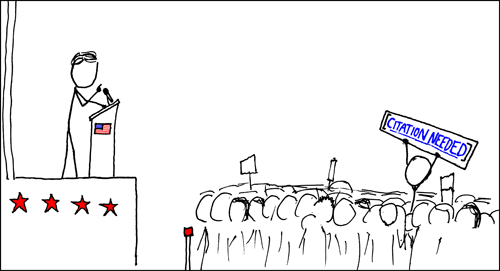
\includegraphics[width=\textwidth]{protester.png}\\
There are \arabic{undefinedreferences} undefined references
\end{center}
\else
No undefined references. Good!
\fi
}


%https://github.com/pads-fhs/LaTeX-Template-Thesis/blob/master/lststyles.tex
\lstdefinelanguage{JavaScript}{
  keywords={typeof, new, true, false, catch,%
    function, return, null, catch, switch, var,%
    if, in, while, do, else, case, break},
  ndkeywords={class, export, boolean, throw, implements, import, this},
  sensitive=false,
  comment=[l]{//},
  morecomment=[s]{/*}{*/},
  morestring=[b]',
  morestring=[b]"
}
\newcommand{\lstsetjavascript}{
  \lstset{
		language=JavaScript,
		breaklines=true,
		commentstyle=\textit,
		basicstyle=\ttfamily,
		keywordstyle=\bfseries,
		stringstyle=\ttfamily,
		showstringspaces=false,
		frame=single,
		tabsize=2
  }
}

\lstdefinelanguage{log}{
  keywords={typeof, new, true, false, catch,%
    function, return, null, catch, switch, var,%
    if, in, while, do, else, case, break},
  ndkeywords={class, export, boolean, throw, implements, import, this},
  sensitive=false,
  comment=[l]{//},
  morecomment=[s]{/*}{*/},
  morestring=[b]',
  morestring=[b]"
}
\newcommand{\lstsetlog}{
  \lstset{
		language=log,
		breaklines=true,
		commentstyle=\textit,
		basicstyle=\ttfamily,
		keywordstyle=\bfseries,
		stringstyle=\ttfamily,
		showstringspaces=false,
		frame=single,
		tabsize=2
  }
}

\lstloadlanguages{Java,XML, JavaScript, log}

\newcommand{\javascriptcode}[4]{
	\lstinputlisting[caption=#2,label=#1, firstline=#3, lastline=#4]{#1.json}
}

\newcommand{\logcode}[4]{
	\lstinputlisting[caption=#2,label=#1, firstline=#3, lastline=#4]{#1.log}
}

\usepackage[bottom]{footmisc} %The footnotes go at the bottom of t\usepackage{dtklogos}he page, instead next to the last line.
%Ajustes para Java
% \lstset{
% 	language=java,
%  	frame=single, % Un marco simple alrededor del código
%     basicstyle=\small\ttfamily, % Utilizar fuente true type pequeña
%     keywordstyle=[1]\color{Blue}\bf, % Funciones en negrita y azul
%     keywordstyle=[2]\color{Purple}, % Argumentos en morado
%     keywordstyle=[3]\color{Blue}\underbar, % Funciones personalizadas subrayadas en azul
%     identifierstyle=, % Nada especial acerca de identificadores
%     commentstyle=\usefont{T1}{pcr}{m}{sl}\color{Green}\small, % Los comentarios se renderizan en fuente pequeña verde
%     stringstyle=\color{Purple}, % Cadenas en morado
%     showstringspaces=false, % No se muestran los espacios entre cadenas
%     tabsize=5, % 5 espacios por tabulado
%     %
%     % Put standard Perl functions not included in the default language here
%     %morekeywords={rand},
%     %
%     % Put Perl function parameters here
%     %morekeywords=[2]{on, off, interp},
%     %
%     % Put user defined functions here
%     %morekeywords=[3]{test},\usepackage{dtklogos}
%    	%
%     morecomment=[l][\color{Blue}]{...}, % Line continuation (...) like blue comment
%     numbers=left, % Número de línea a la izquierda
%     firstnumber=1, % Número de línea comienza en 1
%     numberstyle=\tiny\color{Blue}, % Los números de línea son azules y pequeños
%     stepnumber=5, % Los números de línea van de 5 en 5
%     breaklines=true % Salto de línea si el texto no entra. See http://stackoverflow.com/a/1875803
% }

%\usepackage{xltxtra} % XeLaTeX logo. Yep, just that
%http://tex.stackexchange.com/a/73179/76599
\usepackage{metalogo}
%\usepackage{dtklogos} %BibTeX logo
\def\BibTeX{{\rm B\kern-.05em{\sc i\kern-.025em b}\kern-.08em
    T\kern-.1667em\lower.7ex\hbox{E}\kern-.125emX}}

\newenvironment{alignedDescription}[2][0pt]
  {\begin{list}{}%
    {\renewcommand\makelabel[1]{\textsf{\textbf{##1}}\hfil}%
     \settowidth\labelwidth{\makelabel{#2}}%
     \setlength\leftmargin{\labelwidth+\labelsep + #1}}}%
  {\end{list}}

\newenvironment{elements}
{\begin{quote}\itshape\centering\small}
{\end{quote}}

\newenvironment{cabstract}
{\begin{quote}\itshape\centering\small}
{\end{quote}}

%\usepackage[xindy]{glossaries}
%\newcommand{\chapterabstract}{1}{
%	\begin{center}
%	\small\textit
%	#1
%	\end{center}
%}

\usepackage{xcolor,colortbl}

%\usepackage{lscape}
\usepackage{pdflscape}
\usepackage{float}
\usepackage{fontspec}

%\setmainfont{FreeSerif}
%\setsansfont{FreeSans}
%\setmonofont{Courier}
%\usepackage{fontspec}
%\setmainfont[Ligatures=TeX,Scale=0.95]{Courier}
%\usepackage{blindtext}

\linespread{0.95833} % 11.5/12
\begin{document}

\newcommand{\nombre}{Diseño e implementación de un sistema de computación distribuida con
Raspberry Pi, y estudio comparativo del mismo frente a otras soluciones}
\frontmatter      % Begin Roman style (i, ii, iii, iv...) page numbering


\newcommand{\autor}{Diego Martín Arroyo}
\universityseal{Figures/logousalcolor}

% Set up the Title Page
\title  {\nombre}
\authors  {
            {Diego Martín Arroyo}
            }
\addresses  {\groupname\\\deptname\\\univname}  % These must be set in the "Thesis.cls" file
\date       {\today}
\subject    {}
\keywords   {}

\supervisors{Rodrigo Santamaría Vicente\\ José Andrés Vicente Lober}
\hypersetup{urlcolor=usalred,
           linkcolor={usalred},
           citecolor={usalred},
           urlcolor={usalred},
           anchorcolor={usalred},
           filecolor={usalred}}
\maketitle

%% ----------------------------------------------------------------

\setstretch{1.3}  % It is better to have smaller font and larger line spacing than the other way round

% Define the page headers using the FancyHdr package and set up for one-sided printing
\fancyhead{}  % Clears all page headers and footers
\rhead{\thepage}  % Sets the right side header to show the page number
\lhead{}  % Clears the left side page header

\pagestyle{fancy}  % Finally, use the "fancy" page style to implement the FancyHdr headers

\addtotoc{Acreditación}
\lhead{\emph{Acreditación}}
D. Rodrigo Santamaría Vicente y D. José Andrés Vicente Lober, miembros de la\\ Universidad de Salamanca

\vspace{20 mm}

CERTIFICAN:

\vspace{20 mm}

Que el trabajo titulado ``Diseño e implementación de un sistema de computación distribuida con
Raspberry Pi, y estudio comparativo del mismo frente a otras soluciones'' ha sido realizado por D. Diego Martín Arroyo, con DNI 70825993T y constituye la memoria del trabajo realizado para la superación de la asignatura Trabajo de Fin de Grado de la Titulación Grado en Ingeniería Informática de esta Universidad.

\vspace{10 mm}

Y para que así conste a todos los efectos oportunos.

\vspace{15 mm}

En Salamanca, a 30 de junio de 2015

\vspace{20 mm}

\begin{minipage}[c][5cm]{.45\textwidth}
$\overline{\mbox{Rodrigo Santamaría Vicente}}$\\
Dpto. de Informática y Automática\\
Universidad de Salamanca
\end{minipage}
\hspace{0.5cm}
\begin{minipage}[c][5cm]{.45\textwidth}
\vspace{17pt}
$\overline{\mbox{José Andrés Vicente Lober}}$\\
Dpto. de Informática y Automática\\
Universidad de Salamanca\\
\end{minipage}


%% ----------------------------------------------------------------
% Declaration Page required for the Thesis, your institution may give you a different text to place here
\Declaration{

\addtocontents{toc}{\vspace{1em}}  % Add a gap in the Contents, for aesthetics

Yo, \autor, declaro que la autoría de este Trabajo de Fin de Grado titulado, `\nombre' y el trabajo presentado en el mismo corresponde a mi persona. Confirmo que:

\begin{itemize} 
\item[\tiny{$\blacksquare$}] Este trabajo fue realizado completamente durante mis estudios del Grado en Ingeniería Informática en la Universidad de Salamanca.
 
\item[\tiny{$\blacksquare$}] En aquellas partes de este Trabajo que han sido previamente presentadas como Trabajo de Fin de Grado o cualquier otro tipo de disertación en esta Universidad u cualquier otra institución, esto ha sido claramente indicado.
 
\item[\tiny{$\blacksquare$}] Que todo el trabajo de terceros que ha sido consultado ha sido apropiadamente atribuido.

\item[\tiny{$\blacksquare$}] Donde haya citado el trabajo de otros, la fuente ha sido siempre dada. A excepción de dichas citas, todo el conjunto del Trabajo ha sido realizado por mí.
 
\item[\tiny{$\blacksquare$}] He reconocido todas aquellas fuentes de ayuda.
 
\item[\tiny{$\blacksquare$}] Donde mi Trabajo ha sido parte de una colaboración con otras personas, he indicado claramente la extensión de mi trabajo y el de dichos terceros.
\\
\end{itemize}
 
 
Firmado:\\
\rule[1em]{25em}{0.5pt}  % This prints a line for the signature
 
Fecha:\\
\rule[1em]{25em}{0.5pt}  % This prints a line to write the date
}
\clearpage  % Declaration ended, now start a new page

%% ----------------------------------------------------------------
% The "Funny Quote Page"
\pagestyle{empty}  % No headers or footers for the following pages

\null\vfill
% Now comes the "Funny Quote", written in italics
\textit{``Write a funny quote here.''}

\begin{flushright}
If the quote is taken from someone, their name goes here
\end{flushright}

\vfill\vfill\vfill\vfill\vfill\vfill\null
\clearpage  % Funny Quote page ended, start a new page
%% ----------------------------------------------------------------

\addtotoc{Resumen}  % Add the "Abstract" page entry to the Contents
\abstract{
%\addtocontents{toc}{\vspace{1em}}  % Add a gap in the Contents, for aesthetics

El uso de un sistema distribuido como alternativa económica a un equipo de altas prestaciones es una práctica aprovechada desde hace décadas todo tipo de entornos. El auge actual de sistemas embebidos con gran potencia de cálculo y bajo coste en ha motivado su utilización para la construcción de este tipo de sistemas de computación. Sin embargo, la mayoría de las soluciones responden a una necesidad específica. En el presente documento y los anexos que lo acompañan se plantea y desarrolla la creación de un sistema distribuido compuesto por placas Raspberry Pi que es aprovechable por un gran rango de usuarios con diferentes necesidades (investigadores, desarrolladores, estudiantes\dots), destacando su papel como herramienta didáctica. El resultado final consiste en un sistema escalable y autoconfigurado que incluye un amplio abanico de herramientas de desarrollo de algoritmos distribuidos.

Todas las herramientas creadas cumplen los requisitos de transparencia encontrados en cualquier sistema distribuido. Sumado a su carácter autoconfigurado, el sistema es una solución autosuficiente que gracias al uso de diferentes mecanismos de optimización, hace de este una herramienta de coste mínimo una herramienta con una gran potencia de cálculo.

La construcción del sistema ha implicado el desarrollo de protocolos, utilidades y aplicaciones en diferentes capas, desde servicios provistos por el sistema operativo, pasando por utilidades consumibles por aplicaciones hasta aplicaciones que interactúan con usuarios finales. Todas estas adiciones son transparentes al usuario y altamente integrables con \textit{software} preexistente.

El proceso de desarrollo es precedido por una serie de etapas de evaluación y de un estudio de las diferentes alternativas valoradas. Otro de los frutos del desarrollo del sistema es, por tanto, un estudio comparativo de diferentes propuestas de solución a un problema concreto y de interés en diversas áreas de las Ciencias de la Computación. El carácter didáctico del sistema es también un aspecto clave del desarrollo, pues uno de los objetivos definidos es su utilización en un contexto universitario, facilitando el análisis, desarrollo y comprensión del paradigma de computación distribuida.

\textbf{Palabras clave}: \textit{zeroconf}, sistema distribuido, plataforma orientada a servicios, enseñanza, marcopolo, raspberry pi, python.
}

\clearpage

\addtotoc{\textit{Abstract}}  % Add the "Abstract" page entry to the Contents
\englishabstract{
\addtocontents{toc}{\vspace{1em}}  % Add a gap in the Contents, for aesthetics

The usage of distributed systems as an economic alternative to a high performace computers is a practice applied in all sorts of environments for decades. The ongoing rise of embedded systems with great computational power and low cost has triggered their usage for that sort of computational systems. However, the majority of proposals are focused on a specific need. This document and the attached appendices, annexes and technical documents cover the design and development of a distributed system made of Raspberry Pi boards which is usable by a broader range of users with different needs (researchers, developers, students\dots), featuring its role as a didactic tool. The final result is a scalable and autoconfigured system featuring a big set of distributed algorithms development tools.

All the development tools fulfill the typical transparency requirements found in any distributed system. Added to its autoconfigured nature, the system is a self-sustaining solution which, thanks to several optimization mechanisms, offers a big computing power with very little cost.

The development of the system involves the creation of protocolos, utilities and applications in a layered architecture, from operating system services and utilities to user applications. All the internals are transparent to the user and highly compatible with preexisting software.

The development process is preceded by a series of evaluation phases and an analysis on different alternatives. One of the deliverables of the project is therefore a comparative study on several proposals to a this problem.

Another key component of the development process is the didactic focus of the system. One of the main goals is the usage of the product in a college environment, easing the analysis, development and understanding of the Distributed Computation paradigm fundamentals.

\textbf{Keywordks}: zeroconf, distributed system, service-oriented architecture, teaching, marcopolo, raspberry pi, python.

}

\clearpage  % Abstract ended, start a new page

%% ----------------------------------------------------------------

\setstretch{1.3}  % Reset the line-spacing to 1.3 for body text (if it has changed)

% The Acknowledgements page, for thanking everyone
\acknowledgements{
\addtocontents{toc}{\vspace{1em}}  % Add a gap in the Contents, for aesthetics

The acknowledgements and the people to thank go here, don't forget to include your project advisor\ldots

}
\clearpage  % End of the Acknowledgements
%% ----------------------------------------------------------------

\hypersetup{urlcolor=blue,
           linkcolor={blue},
           citecolor={blue},
           urlcolor={blue},
           anchorcolor={blue},
           filecolor={blue}}

\pagestyle{fancy}  %The page style headers have been "empty" all this time, now use the "fancy" headers as defined before to bring them back


%% ----------------------------------------------------------------
\lhead{\emph{Contenidos}}  % Set the left side page header to "Contents"
\tableofcontents  % Write out the Table of Contents

%% ----------------------------------------------------------------
\lhead{\emph{Lista de figuras}}  % Set the left side page header to "List if Figures"
\listoffigures  % Write out the List of Figures

%% ----------------------------------------------------------------
\lhead{\emph{Lista de tablas}}  % Set the left side page header to "List of Tables"
\listoftables  % Write out the List of Tables

%% ----------------------------------------------------------------
%\setstretch{1.5}  % Set the line spacing to 1.5, this makes the following tables easier to read
%\clearpage  % Start a new page
%\lhead{\emph{Lista de abreviaturas}}  % Set the left side page header to "Abbreviations"

% \listofsymbols{ll}  % Include a list of Abbreviations (a table of two columns)
{
%TODO: See : ftp://ftp.tex.ac.uk/ctan/tex-archive/macros/latex/contrib/listofsymbols/listofsymbols.pdf
% \textbf{Acronym} & \textbf{W}hat (it) \textbf{S}tands \textbf{F}or \\
\textbf{IEEE} & \textbf{I}nstitute of \textbf{E}lectrical and \textbf{E}lectronic \textbf{E}ngineers \\
\textbf{NTP} & \textbf{N}etwork \textbf{Time} \textbf{P}rotocol \\
\textbf{DHCP} & \textbf{D}ynamic \textbf{H}ost \textbf{C}onfiguration \textbf{P}rotocol\\
\textbf{mDNS} & \textbf{M}ulticast \textbf{D}omain \textbf{N}ame \textbf{S}ystem\\
}

%%% ----------------------------------------------------------------
\clearpage  % Start a new page
\lhead{\emph{Physical Constants}}  % Set the left side page header to "Physical Constants"
\listofconstants{lrcl}  % Include a list of Physical Constants (a four column table)
{
% Constant Name & Symbol & = & Constant Value (with units) \\
Speed of Light & $c$ & $=$ & $2.997\ 924\ 58\times10^{8}\ \mbox{ms}^{-\mbox{s}}$ (exact)\\

}

%% ----------------------------------------------------------------
\clearpage  %Start a new page
\lhead{\emph{Symbols}}  % Set the left side page header to "Symbols"
\listofnomenclature{lll}  % Include a list of Symbols (a three column table)
{
% symbol & name & unit \\
$a$ & distance & m \\
$P$ & power & W (Js$^{-1}$) \\
& & \\ % Gap to separate the Roman symbols from the Greek
$\omega$ & angular frequency & rads$^{-1}$ \\
}
%% ----------------------------------------------------------------
% End of the pre-able, contents and lists of things

% Begin the Dedication page

\setstretch{1.3}  % Return the line spacing back to 1.3

\pagestyle{empty}  % Page style needs to be empty for this page
\dedicatory{For/Dedicated to/To my\ldots}

\addtocontents{toc}{\vspace{2em}}  % Add a gap in the Contents, for aesthetics

%\hypersetup{urlcolor=blue, colorlinks=true}

%% ----------------------------------------------------------------
\mainmatter	  % Begin normal, numeric (1,2,3...) page numbering
\pagestyle{fancy}  % Return the page headers back to the "fancy" style

% Include the chapters of the thesis, as separate files
% Just uncomment the lines as you write the chapters
\lhead{\emph{Introducción}}
\chapter{Introducción}

Los límites físicos de los que adolecen los computadores en la actualidad\cite{seth:physical} hacen de la computación distribuida un recurso para incrementar de forma sencilla y económica el rendimiento total de un sistema. Sumado a estos beneficios, el auge de sistemas como teléfonos inteligentes o aplicaciones web ha potenciado el auge de diferentes paradigmas distribuidos en los últimos años.
%TODO\citationneeded[https://vsis-www.informatik.uni-hamburg.de/getDoc.php/publications/432/activecomponents.pdf]. 

Sin embargo, estas ganancias conllevan una serie de inconvenientes entre los que figura el aumento de la complejidad del sistema. En general, un sistema distribuido requiere un conjunto de entidades independientes, más difíciles de configurar y mantener que una única entidad. Además, aparecen nuevos problemas: comunicación, integridad y sincronización, dificultad en el desarrollo y depuración de aplicaciones, etcétera.

En el apartado didáctico, el estudio del paradigma distribuido suele requerir un gran esfuerzo por parte de los estudiantes, en particular a la hora de comprender los fundamentos básicos de cualquier aplicación distribuida así como a la hora de realizar tareas de análisis y depuración.

La presente memoria recoge el proceso de evaluación de diferentes alternativas para la creación de un sistema distribuido que satisfaga un conjunto de necesidades previamente establecidas, así como las diferentes etapas de diseño y desarrollo de un sistema formado por dispositivos Raspberry Pi como propuesta de solución y la creación de un conjunto de protocolos, herramientas y servicios para la utilización del mismo como utilidad de investigación en el campo de la computación distribuida y como herramienta didáctica para disciplinas relacionadas con dicho área.

El sistema se compone de un conjunto de dispositivos físicos compuesto por los nodos de computación y una serie de módulos accesorios, así como los diferentes mecanismos de alimentación y refrigeración, un conjunto de herramientas \textit{software} que permiten la coordinación y comunicación entre los diferentes procesos y una serie de herramientas que facilitan el trabajo con el sistema.

Además, se incluyen las definiciones de los diferentes conceptos teóricos necesarios para la creación del sistema, así como las diferentes etapas de aprendizaje, evaluación de alternativas y diferentes procesos de evaluación llevados a cabo durante las diferentes etapas desarrollo, así como las metodologías de trabajo utilizadas, sin olvidar la documentación de todas las herramientas creadas. %Introducción

\lhead{\emph{Motivación y objetivos}}
\chapter{Motivación y objetivos}

\begin{cabstract}
En el que se describe la motivación que lleva al desarrollo de este Trabajo y se describen en detalles los objetivos del sistema como un todo.
\end{cabstract}

El presente proyecto responde al interés personal en las áreas de conocimiento relacionadas con la Computación Distribuida. La propuesta final cuenta con un atractivo añadido, que es la utilización de computadores embebidos, generalmente no considerados como integrantes de un sistema distribuido. En diferentes reuniones entre las diferentes partes se terminan de perfilar los diferentes objetivos a completar, entre los que destaca la potencial integración del sistema en asignaturas del plan de estudios del Grado en Ingeniería Informática como herramienta didáctica.

\section{Objetivos}

El sistema creado se inspira en proyectos similares (descritos en \ref{stateoftheart}) y se diseña con el objetivo de dar solución a diferentes necesidades identificadas como estudiante de varias asignaturas del currículo del Grado en Ingeniería Informática. El sistema cuenta con cuatro objetivos a alto nivel independientes:

\begin{itemize}
	\item Como síntesis de los conocimientos adquiridos en la carrera, se busca la creación de un sistema completo desde sus cimientos hasta los componentes de más alto nivel, gestionando las tareas de mantenimiento, instalación y manejo del mismo, así como los protocolos de trabajo, tanto en cada uno de los componentes del sistema como en la comunicación entre los mismos. Con un enfoque más teórico, se pretende crear un sistema capaz de poder ser utilizado como herramienta de diseño y prueba de algoritmos que resuelvan problemas aprovechando la distribución de tareas, así como el análisis de dichos algoritmos utilizando versiones finales del sistema.

	\item Potenciar su uso como herramienta de aprendizaje en las áreas de conocimiento Sistemas Operativos, Algoritmia, Redes de Computadores, Sistemas Distribuidos, Administración de Sistemas y Sistemas Embebidos.
	
	\item Constituir una herramienta didáctica para varias asignaturas del currículo del Grado en Ingeniería Informática de la Universidad de Salamanca, analizando aquellas relevantes y proponiendo soluciones a las diferentes necesidades propuestas por el Profesorado, Estudiantes y Administradores en colaboración con dichas partes.

	\item Intentar elevar el \textit{state of the art} en el mundo de los sistemas distribuidos con plataformas embebidas mediante la creación de un sistema multipropósito en lugar de soluciones con un fin determinado, que constituyen la tendencia actual.
\end{itemize}

Partiendo de la premisa de las potenciales ventajas del uso de este tipo de computadores se plantea el sistema definitivo (en \ref{alternativas} se detalla el proceso de decisión), no sin antes realizar una etapa de evaluación de las diferentes alternativas.

\section{Objetivos del sistema}

Durante las fases de definición del proyecto, se plantean los siguientes objetivos concretos para la propuesta de solución elegida a cumplir.

\subsection{Diseño y construcción de la arquitectura física del sistema}

Se deberán definir las interconexiones físicas entre los diferentes componentes del sistema, proponer soluciones a los diferentes aspectos físicos del sistema, tales como la alimentación eléctrica, conexiones de red o la refrigeración, entre otros, analizando los diferentes enfoques y valorando la mejor solución en función del resto de objetivos a cumplir y las restricciones (tiempo, coste) planteadas.

\subsection{Arquitectura multipropósito orientada a servicios}

El principal propósito del sistema creado será el alojamiento de un conjunto de aplicaciones (servicios) en el mismo, que podrán ser aprovechados por diferentes usuarios para explotar la capacidad de cálculo de las máquinas.

Sin embargo, una de las características de los sistemas similares al que se modela es su orientación a un único fin concreto. Se plantea crear un sistema que rompa con esta tendencia, siendo capaz de dar cabida a diferentes tipos de aplicaciones.

\subsection{Gestión del sistema}

El sistema debe contar con un conjunto de herramientas que mantengan los principios de transparencia propios de un sistema distribuido (ver \ref{transparencia}), y su gestión debe ser sencilla para los responsables de la misma (personal de administración).

\subsection{Integración}

El sistema debe integrarse en una infraestructura preexistente, la presente en la Facultad de Ciencias de la Universidad de Salamanca, sin que dicha integración comprometa el diseño básico del sistema a fin de facilitar su adaptabilidad a otros entornos (ver \ref{infraestructura}). Es necesario por tanto realizar pruebas que evalúen el rendimiento del sistema creado en la misma\footnote {Con el objetivo de facilitar dicha integración, el sistema se desarrolla parcialmente aprovechando la infraestructura presente.}.

A fin de facilitar el uso del sistema por los usuarios finales, se deberán utilizar los recursos ofrecidos por la infraestructura en aquellos casos que sea posible para tareas como la conexión de red, gestión de usuarios\footnote{Existe un directorio de autenticación preexistente en el que todo miembro de la organización cuenta con unas credenciales.}, etcétera.% % Para la integración de dicho directorio se utiliza \textbf{nsswitch} (ver \ref{nsswitch}). 

\subsection{Uso como herramienta didáctica}

El sistema debe ofrecer una serie de ventajas a las herramientas didácticas utilizadas en aquellas asignaturas donde se impartan conocimientos relacionados con la computación paralela y distribuida, ofreciendo herramientas que faciliten la comprensión de dichos paradigmas o el desarrollo, prueba y aplicación de programas basados en los mismos. Se crearán de aplicaciones y herramientas como alternativas a las utilizadas actualmente, analizando las demandas de los usuarios, así como pruebas de concepto que garanticen que las diferentes tareas encargadas a los sistemas actuales serán integrables en la propuesta de solución.

\subsection{Evaluación}

A fin de probar los objetivos definidos anteriormente, la viabilidad de sistema como herramienta didáctica y su integración en la organización deberán ser determinados por los diferentes usuarios de la misma y la realización de pruebas de integración.

Durante el desarrollo del proyecto se añaden los siguientes objetivos funcionales:

\subsection{\textit{Zeroconf}}

El sistema debe configurarse de forma automática (\textit{zeroconf}) en cualquier tipo de circunstancia (sin que el número de nodos o la configuración de la red sean aspectos relevantes, por ejemplo). Para ello se deberán utilizar o crear una serie de herramientas que posibiliten esta propiedad del sistema. Entre estas herramientas destaca como elemento clave la utilización de un protocolo de descubrimiento de nodos y servicios. Como se destaca en apartados posteriores de la memoria, se ha optado por la creación de este en lugar de utilizar una alternativa de terceros, recibiendo el nombre \textit{MarcoPolo} (ver \ref{marcopolo}).

\subsection{\textit{Test-Driven Development}}

El desarrollo de las diferentes herramientas \textit{software} se deberá realizar bajo los principios del desarrollo conducido por pruebas (ver \ref{tdd}) como mecanismo para la detección temprana de errores, automatizando este tipo de dinámica en todos los casos en los que sea posible.

\vspace{2cm}

En conclusión, los objetivos del proyecto son los siguientes:

\begin{hyphenrules}{nohyphenation}
\begin{center}
\itshape
\begin{itemize}
	\item[] Diseñar un sistema distribuido no jerárquico autoconfigurado e integrable en una infraestructura existente.
	\item[] Crear un conjunto de herramientas, protocolos y aplicaciones para la explotación de los recursos que ofrece el sistema.
	\item[] Orientar la explotación del mismo como herramienta de diseño y prueba de algoritmos.
	\item[] Explotar las posibilidades didácticas del sistema.
	\item[] Analizar las ventajas e inconvenientes del sistema frente a otras soluciones similares.
	\item[] Analizar la efectividad de la solución propuesta mediante herramientas de evaluación.
\end{itemize}
\end{center}
\end{hyphenrules} % Motivación y objetivos

\lhead{\emph{Conceptos teóricos}}

\chapter{Conceptos teóricos}

\section{Programación orientada a eventos}
\label{eventdriven}
\section{Computación distribuida}

Un sistema distribuido es aquel conformado por un conjunto de nodos independientes que son percibidos como una entidad única y coherente por el usuario final. Dicha definición implica dos conceptos de importancia en el paradigma:

\begin{itemize}
  \item Autonomía: los diferentes integrantes del sistema cuentan con un alto grado de autonomía entre sí, y por tanto se deben diseñar e implementar mecanismos de comunicación entre los mismos, mecanismos que formarán parte del núcleo del sistema, y cuyo diseño tendrá consecuencias directas en el funcionamiento final del sistema.
  \item Transparencia: Las diferencias entre diferentes nodos suelen ser invisibles para los usuarios finales, así como la gestión de fallos y recuperación y la uniformidad a la hora de interactuar con el sistema. Según \citationneeded las siguientes propiedades del sistema deben contar con un grado de transparencia alto\footnote{En numerosas ocasiones las propiedades de un sistema hacen desfavorable el cumplimiento de todos los requisitos de transparencia. Un ejemplo sería la transparencia de relocación en el sistema DNS.}:
  \subitem \textbf{Acceso}: La forma de almacenamiento y gestión de los recursos e información presentes en el sistema debe ser completamente transparente.
  \subitem \textbf{Localización}: La localización física del sistema no debe ser de relevancia para el uso del mismo.
  \subitem \textbf{Migración}: El cambio de plataforma de un sistema debe ser transparente para el usuario (ejemplo: cambio del sistema operativo).
  \subitem \textbf{Relocación}: El hecho de que un sistema se esté trasladando de un lugar a otro no debe afectar al usuario final.
  \subitem \textbf{Replicación}: El numero de elementos redundantes en un sistema es desconocido para el usuario final.
  \subitem \textbf{Concurrencia}: Un usuario no debe percibir la presencia de otros agentes interactuando con el sistema.
  \subitem \textbf{Gestión de errores}: En caso de fallo, el usuario final no debe percibir el mismo, ni el proceso de recuperación consecuente.
\end{itemize}

Generalmente los sistemas distribuidos son fácilmente escalables gracias a la autonomía de cada nodo, y los mecanismos de transparencia permiten crear sistemas heterogéneos de forma sencilla, en ocasiones apoyados en capas \textit{middleware} que posibilitan dicha transparencia.

Otro concepto importante en el desarrollo de sistemas distribuidos es la ``apertura'' (\textit{openness}) de los mismos. Un sistema ofrece una serie de servicios gracias al uso de un conjunto de reglas conocidas por todos los participantes, generalmente recogidos en estándares de acceso público que definen la sintaxis y semántica de los servicios, conocidos como lenguajes de especificación de interfaz (\textit{Interface Definition Language}). Si dicho lenguaje es definido de forma apropiada, es posible crear diferentes implementaciones del mismo que sean capaces de comunicarse entre sí, incluso ejecutándose sobre máquinas completamente diferentes
%To achieve flexibility in open distributed systems, it is crucial that the system is organized as a collection of relatively small and easily replaceable or adaptable components. This implies that we should provide definitions not only for the highest-level interfaces, that is, those seen "by users and applications, but also definitions for interfaces to internal parts pJ the system and describe how those parts interact. This approach is relatively new. Many older and even contemporary systems are constructed using a monolithic approach in which components  (Tanenbaum, p8)

\subsection{Escalabilidad}

La escalabilidad del sistema en ocasiones se ve afectada por las decisiones de diseño llevadas a cabo. En arquitecturas centralizadas el punto principal del sistema consituye un ``cuello de botella'' evidente que define un límite en el crecimiento del sistema. La disposición geográfica exige una serie de consideraciones adicionales, entre las que se encuentra la latencia del sistema.

\subsection{Algoritmos distribuidos}

Un algoritmo distribuido es aquel que realiza una tarea de forma distribuida, cumpliendo el siguiente conjunto de propiedades:

\begin{itemize}
\item Ningún componente conoce el total de la información sobre el estado del sistema (principio de autonomía).
\item Un componente únicamente puede tomar decisiones basadas en su conocimiento local (principio de autonomía).
\item El fallo de un nodo no provoca el fallo del sistema (transparencia).
\item No hay una asunción implícita de que existe un reloj global.
\end{itemize}

\subsection{Modelos arquitectónicos}

Existe un gran rango de diferentes modelos de construcción de sistemas distribuidos en función de las necesidades a cubrir por el sistema.

%Tanenbaum 2.1

\subsubsection{Clúster}

En general se conoce como clúster al conjunto de nodos homogéneos y dispuestos físicamente en la misma localización, conectados entre sí mediante mecanismos fiables como redes de área local y que cuentan con el mismo conjunto de herramientas (en particular el sistema operativo). Generalmente estos sistemas se componen de nodos de bajo coste, como equipos de escritorio (denominados \textit{Commodity Off-The-Shell})\citationneeded{http://en.wikipedia.org/wiki/Commodity\_computing} y son utilizados para la realización de una única tarea con un coste computacional alto en paralelo.


\write18{wget -O Chapters/Chapter2/Figures/Beowulf.png -nc   http://upload.wikimedia.org/wikipedia/commons/4/40/Beowulf.png?download}

\begin{figure}[H]
\centering
\includegraphics[width=0.7\textwidth]{Chapter2/Figures/Beowulf.png}
\caption{Esquema de un clúster Beowulf, un tipo de clúster}
\label{fig:beowulf}
\end{figure}

\subsubsection{\textit{Grid}}

Una ``rejilla'' (grid) es un sistema distribuido en el que los nodos del sistema no son homogéneos y cuentan con diferentes características. Los mecanismos de transparencia descritos anteriormente son clave para el correcto funcionamiento del sistema y las interconexiones entre los diferentes elementos.


\subsubsection{Sistemas de información distribuida}

\subsubsection{Sistemas descentralizados}

Uno de los problemas de las arquitecturas propuestas es la dependencia de un nodo que actúe de coordinador para el resto de los nodos del sistema.

\subsection{Seguridad}

Las medidas de seguridad a tomar dependen de las propiedades y objetivos propios del sistema: en general sistemas utilizados dentro de una organización y una infraestructura sin interacción con entornos no controlados suelen contar con un número menor de medidas de seguridad que aquellos utilizados en entornos ``hostiles'', y la seguridad depende de la confianza depositada en la administración del sistema. Sin embargo, un sistema de este tipo es vulnerable a ataques internos por parte de usuarios o intrusiones en la infraestructura.

Un sistema integrado en un entorno hostil debe además vigilar cualquier tipo de potencial ataque malicioso y controlar el acceso al sistema de forma más minuciosa.

\subsection{Integridad}

\subsection{Comunicación}

\subsection{Distribución}

Uno de los modelos típicos en el desarrollo de sistemas distribuidos es el ``divide y vencerás'': la división de un problema en múltiples tareas y la distribución de las mismas entre los diferentes componentes del sistema, reagrupando los resultados posteriormente. Dicho paradigma no se aplica únicamente a tarea a realizar, sino también al conjunto de datos sobre el que realizarla, paralelizando una misma operación en diferentes nodos sobre fragmentos del conjunto de datos sobre el que operar, recopilando los datos devueltos y conformando la respuesta final.

\write18{wget -P Chapters/Chapter2/Figures/ -nc http://upload.wikimedia.org/wikipedia/commons/6/6d/Mapreduce.png}

\begin{figure}[H]
\centering
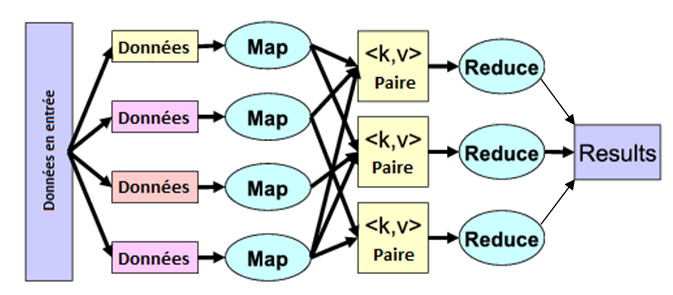
\includegraphics[width=0.7\textwidth]{Chapter2/Figures/Mapreduce.png}
\caption{\textbf{MapReduce} se basa en el principio de la distribución de los datos sobre diferentes nodos (\textit{Map}) y la recopilación de los datos procesados (\textit{Reduce})}
\label{fig:mapreduce}
\end{figure}

\subsection{Autoadministración}

%2.4 SELF -MANAGEMENT IN DISTRIBUTED SYSTEMS 

\section{Paralelización, \textit{threads}}
\section{Multicasting}

\section{WebSockets}

\section{Test-Driven Development}


\section{PAM}

\section{Cross-compiling}

\section{Python}

\lhead{\emph{Dominio del problema}}
\chapter{Dominio del problema}

La utilización de algoritmos distribuidos implica mejoras sustanciales en una gran cantidad de aplicaciones, incrementando la capacidad global de computación de un sistema mediante la unión de varios dispositivos de cómputo que trabajan de como una única unidad indivisible a la vez que mantienen un alto grado de independencia y una tolerancia global a fallos muy alta. Sin embargo, el desarrollo de aplicaciones distribuidas implica el uso de un conjunto de nodos cuyo coste y mantenimiento es costoso.

Dicho aumento de la potencia implica una mayor complejidad en el desarrollo de algoritmos que puedan aprovechar de forma óptima este tipo de sistemas. Varios factores como la sincronización y la comunicación entre partes, o errores tales como condiciones de carrera son mucho más comunes que en otro tipo de aplicaciones. Dichas dircunstancias no solo dificultan el desarrollo de este sistema, sino también la comprensión de los fundamentos básicos de la Computación Distribuida. %cite http://ceit.aut.ac.ir/~amirkhani/Downloads/patterson_book.pdf

Si bien la mayoría de las aplicaciones en las que el paradigma de computación distribuida introduce mejoras suelen exigir una gran capacidad de cálculo, su desarrollo únicamente requiere un conjunto de instancias independientes de un software (sistema operativo, contenedor de servicios...) con las que trabajar. Dicha característica implica que la utilización de nodos de precio reducido (o incluso reutilizados) para el diseño, análisis y evaluación de este tipo de algoritmos constituye una alternativa válida frente a sistemas de precio superior.

Sumada a dicha motivación existe el potencial aprovechamiento de este sistema como herramienta didáctica que facilite el aprendizaje de conceptos como el reparto de procesos, balance de carga o la compartición de recursos en asignaturas centradas en este tipo de conceptos dentro de los planes de estudio de Ingeniería Informática o titulaciones afines.

Con el presente proyecto se plantea la creación de un sistema con estas características aprovechando el bajo coste de los componentes del mismo que permita en primer lugar su utilización como herramienta de análisis y diseño (o incluso su utilización como plataforma definitiva) de aplicaciones distribuidas y en segundo lugar la posibilidad de uso como herramienta educativa.

A la hora de crear el sistema se realiza un análisis de las diferentes alternativas, a fin de escoger la alternativa que mejor satisfaga los objetivos definidos.

Figura: Tabla de alternativas

\section{Objetivos del proyecto}

Este proyecto cuenta con varios objetivos muy diferentes entre sí, que se agrupan en tres categorías:
\begin{itemize}
  \item Arquitectura subyacente\\
  Definición de los componentes hardware a utilizar en el sistema, interconexión de los mismos, soluciones de alimentación eléctrica, almacenamiento\dots.
  \item Servicios a proveer\\
  Conjunto de servicios que podrán ser aprovechados por diferentes clientes para explotar la capacidad de cálculo de las máquinas.
  \item Componente didáctico\\
  Creación de aplicaciones, herramientas y documentación como alternativa a las instalaciones típicas utilizadas actualmente.
\end{itemize}

\section{Definiciones}

\subsection{Definición del dominio del problema}

El sistema se ubica en una Facultad universitaria con aproximadamente 600 alumnos\citationneeded con varias asignaturas en las que se imparten áreas de conocimiento relacionados con la Computación Distribuida, en particular las asignaturas \textbf{Arquitectura de Computadores} y \textbf{Sistemas Distribuidos} \cite{DIA15GuiaAcademica}.

\subsection{Modelado del sistema actual}

La Facultad cuenta con varias aulas y laboratorios informáticos donde los alumnos disponen de la intraestructura necesaria para realizar los ejercicios y prácticas asignadas. Dichos espacios permiten utilizar cualquier equipo como nodo, pues se integran en la misma red, siendo incluso factible la comunicación directa entre equipos situados en diferentes aulas o incluso edificios. La conexión es relativamente rápida, contando con un cableado capaz de soportar teóricamente transferencias de hasta 100Mb/s de forma bidireccional (\textit{full-duplex}) (\textbf{Cita requerida}). La gestión de un sistema de autenticación se realiza mediante el protocolo LDAP (\textit{Lightweight Directory Access Protocol}) \cite{RFC4516-comment}, contando con un sistema de ficheros centralizado que permite acceder a la información de un usuario desde cualquier equipo, facilitando las tareas de replicación de la información entre nodos.

La mayoría de las prácticas asignadas a los alumnos son desarrolladas en el lenguaje \textbf{Java}, ya conocido por la totalidad de los estudiantes gracias a asignaturas previamente cursadas (\textbf{Cita requerida}) y que facilita el despliegue y la compatibilidad entre diferentes equipos de trabajo sustancialmente. En ocasiones es necesario el uso de lenguajes como C y se plantean alternativas a \textit{Java} como Python o C\#.

\paragraph{Problemas conocidos}

Si bien la infraestructura existente es capaz de proveer a los estudiantes de los recursos necesarios, identificamos una serie de problemas inicialmente:

\begin{itemize}
  \item Cada grupo de alumnos necesita tres estaciones de trabajo para poder realizar algunos de los ejercicios propuestos.
  \item El servidor LDAP constituye un ``cuello de botella'', pues todos los alumnos acceden a él de forma intensiva, provocando el fallo por exceso de peticiones del mismo.
  \item Las técnicas de programación utilizadas hasta la fecha tienen un rendimiento bajo y son en ocasiones relativamente complejas.
\end{itemize}

\subsection{Identificación de usuarios participantes}

\begin{itemize}

  \item Estudiantes de tercero y cuarto curso del Grado en Ingeniería Informática.
  \item Doctentes de las asignaturas Arquitectura de Computadores y Sistemas Distribuidos.
  \item Administradores del Sistema.
\end{itemize}

\section{Identificación de las necesidades de cada parte}
\subsection{Necesidades de los alumnos}

\begin{itemize}
  \item Entorno de trabajo sencillo que agilice el desarrollo de sus prácticas.
  \item Posibilidad de observar los resultados de las ejecuciones de forma sencilla.
  \item Facilidades para el despliegue de los diferentes ejecutables en todas las máquinas, así como el consumo de los servicios que estos implementen.
\end{itemize}

\subsection{Necesidades de los docentes}

\begin{itemize}
  \item Entorno versátil sobre el cual puedan llevarse a cabo la totalidad de las prácticas y ejercicios propuestos, aportando si es posible algún tipo de ventaja sobre el sistema en uso.
\end{itemize}

\subsection{Administrador}

\begin{itemize}
  \item Sistema integrable en la intraestructura actual cuyo mantenimiento sea sencillo y cuyo enfoque garantice la escalabilidad y su durabilidad.
\end{itemize}

\section{Propuestas para la búsqueda de necesidades}

\begin{itemize}
  \item Encuestas o entrevistas a todas las partes.
  \item Evaluación de la experiencia de uso en las diferentes etapas de desarrollo del sistema.
\end{itemize}

\section{Identificación de requisitos}

\subsection{Requisitos de almacenamiento de la información}

\begin{itemize}
  \item Gestión de usuarios (credenciales de autenticación)
  \item Gestión de los datos de cada usuario
  \item \textit{Logs} del sistema
\end{itemize}

\subsection{Identificación de requisitos funcionales}


\subsection{Identificación de requisitos no funcionales}

\begin{itemize}
  \item El \textit{software} debe ser mantenible y robusto\footnote{Siendo dicha robustez garantizada mediante el uso de \textit{software} utilizado por una base de usuarios significativa, una arquitectura conocida, pruebas realizadas sobre él o un equipo de desarrollo en activo, entre otras}.
  \item Reducción de los costes de desarrollo.
  \item Definición de los protocolos de comunicación.
  \item Definición de los protocolos de seguridad y confidencialidad.
  \item Definición de la interacción con el usuario.
  \item Integridad del sistema y fiabilidad (\textit{uptime}, recuperación frente a fallos).
  \item Productos a crear.
  \item Compatibilidad con las prácticas y ejercicios.
\end{itemize}

\section{Evaluación de alternativas}
\label{alternativas}
A la hora de evaluar las diferentes opciones que satisfagan los requisitos descritos, se consideran los siguientes aspectos:

\begin{itemize}
  \item Coste económico.
  \item Prestaciones técnicas (potencia de procesamiento, entrada/salida, capacidad de almacenamiento,facilidad de interconexión con otros materiales...).
  \item Facilidad de trabajo y de aprendizaje (documentación disponible, proyectos similares ya realizados, conocimiento sobre la plataforma en cuestión...).
  \item Escalabilidad del sistema.
  \item Necesidades de mantenimiento del sistema.
  \item Consumo del sistema (consumo eléctrico).
  \item Obsolescencia del sistema (número de años en los que el sistema podrá ser actualizado (tanto en hardware como software) y será capaz de seguir siendo una herramienta adecuada para el propósito planteado).

\end{itemize}

\subsection{Propuesta de solución: Virtualización de entornos de trabajo}

Crear un conjunto de nodos virtuales dentro de una máquina que simulen un sistema distribuido

\paragraph{Ventajas intrínsecas de la solución}

Simplificación del sistema (reduce las necesidades de adquisición y mantenimiento de hardware).
Gestión de varias partes del sistema (sistema de ficheros centralizado, gestión de usuarios...) de forma mas sencilla. El coste se reduce significativamente.

\paragraph{Inconvenientes intrínsecos del sistema}

No se exploran apenas las posibilidades de un sistema distribuido formado por varios equipos físicamente independientes.

\paragraph{Facilidad de trabajo y curva de aprendizaje}

Si bien el trabajo con cada una de las instancias es previsiblemente sencillo, debido a la eliminación de la gran parte del mantenimiento de la capa física subyacente, el uso de este tipo de sistema requiere una etapa de formación previa en materia de virtualización.

\paragraph{Prestaciones técnicas}

Las prestaciones técnicas con las que se contaría, de llevarse a cabo este proyecto, son las de los equipos ya dispuestos para fines similares a este en el Centro: %TODO: Andrés. 

\paragraph{Coste econonómico}

El coste econónomico es muy reducido si ya se cuenta con los equipos a utilizar y las licencias \textit{software} que fueran necesarias para realizar la virtualización.

\paragraph{Escalabilidad del sistema}

Dependiente de las capacidades de virtualización del equipo disponible, y el número de nodos y usuarios a gestionar (previsiblemente alto)

\paragraph{Necesidades de mantenimiento}

Las necesidades propias de un sistema GNU/Linux junto a las específicas de la virtualización de los equipos.

\paragraph{Consumo energético del sistema}
\paragraph{Obsolescencia del sistema}

\paragraph{Material con el que se cuenta actualmente}
Se plantea el aprovechamiento de equipos pertenecientes a la Universidad, por lo que se estima un coste muy pequeño a la hora de adquirir material.
\paragraph{Otras características}

\paragraph{Análisis coste/beneficio}

Si bien el coste de esta solución es muy atractivo, presenta una serie de carencias que dificultan significativamente el desarrollo del sistema en el mismo. 


\subsection{Propuesta de solución: Clúster con equipos de escritorio}

Se plantea la reutilización de equipos de escritorio pertenecientes a la Universidad que ya no se encuentran en uso (debido a su renovación, falta de potencia como PC...) para la creación de este sistema.

\paragraph{Ventajas intrínsecas de la solución}
La potencia del sistema es mucho mayor que la de cualquier otra solución considerada viable. Se reduce dramáticamente el coste de adquisición de material y permite dar un nuevo ciclo de vida a material universitario.
La arquitectura es conocida y fiable.

\paragraph{Inconvenientes intrínsecos del sistema}

No se exploran las características únicas de otros sistemas menos ``convencionales'', tales como la utilización de sistemas embebidos. El consumo energético es mayor, existe una mayor demanda de espacio, que puede dificultar la implementación de diferentes aplicaciones didácticas ya planteadas como objetivo funcional del sistema.

\paragraph{Facilidad de trabajo y curva de aprendizaje}

Soporte completo de casi la totalidad de las distribuciones de GNU/Linux.
Las necesidades de manipulación de hardware se minimizan.

\paragraph{Prestaciones técnicas}
Arquitectura x86/x64
Entre 2 y 4 GB de memoria
Conectividad Ethernet, USB
Almacenamiento en disco duro
\paragraph{Coste econonómico}

El coste económico de dichos equipos es prácticamente nulo, pues ya se cuenta con los mismos y su utilización no exige la adquisición de sustitutos, pues ya habían sido retirados de su uso.

\paragraph{Escalabilidad del sistema}

Dependiente únicamente del coste económico de la adquisición de nuevos equipos, o de la disponibilidad de equipos desechados.

\paragraph{Necesidades de mantenimiento}

Las necesarias en cualquier sistema GNU/Linux y las específicas del montaje dado (en materia de refrigeración, gestión de cableado, etcétera).

\paragraph{Consumo energético del sistema}

El típico de cualquier equipo de escritorio.

\paragraph{Obsolescencia del sistema}

Estos equipos tienen una antigüedad de aproximadamente 4 años. Dicha edad no impide que sean capaces de utilizar aplicaciones actuales, y en general no se prevé la incompatibilidad con ninguna aplicación.

\paragraph{Material con el que se cuenta actualmente}
La Facultad de Ciencias ya dispone de los equipos, pues se plantea la reutilización de los mismos

\paragraph{Otras características}

\paragraph{Análisis coste/beneficio}

Si bien el coste de estos equipos es prácticamente nulo, dicho atractivo contrasta con los potenciales problemas que el uso de estos sistemas puede implicar (dificultad de desarrollo de objetivos funcionales, uso de sistemas convencionales en detrimento de soluciones más innovadoras\dots).

\subsection{Clúster con equipos embebidos multimedia }

Utilización de equipos embebidos diseñados para aplicaciones multimedia en el sistema (ejemplos son Chromecast, Apple TV, Amazon Fire TV...)

\paragraph{Ventajas intrínsecas de la solución}

Relacion potencia/precio presumiblemente superior a soluciones de coste similar como las placas Raspberry Pi.

\paragraph{Inconvenientes intrínsecos del sistema}

Dificultad de conexión (generalmente la conexión a red se realiza de forma inalámbrica, ausencia casi absoluta de cualquier conexión cuya finalidad no sea la emisión de vídeo o conexión con sistemas de almacenamiento mediante USB), falta de puertos GPIO, I2C...

\paragraph{Facilidad de trabajo y curva de aprendizaje}
Es difícil determinar la viabilidad de esta solución, pues no se cuenta con experiencia previa ni una documentación amplia al respecto.
Es probable que sea necesaria la manipulación del sistema a muy bajo nivel. Lo cual incrementa el grado de complejidad de la solución.

\paragraph{Prestaciones técnicas}
Arquitectura ARM
2 núcleos a 1.2 GHz
512 MB de RAM
Almacenamiento: 2 GB no expandibles
Alimentación por microUSB

\paragraph{Coste econonómico}

El coste de estos equipos es reducido, generalmente inferior a 30 € por unidad.

\paragraph{Escalabilidad del sistema}

Dependiente del coste de adquisición de nuevos equipos y las facilidades de interconexión de la plataforma (previsiblemente compleja, debido a la ausencia de sistemas de interconexión más allá de WiFi)

\paragraph{Necesidades de mantenimiento}

Dependiente del número de modificaciones que se realicen a las capas más bajas. En el peor de los casos puede que el administrador del sistema tenga que someterse a una etapa de formación para realizar un mantenimiento adecuado del sistema sin depender de desarrolladores previos.
Las derivadas del mantenimiento de un sistema Linux sumadas a posibles problemas de interconexión si se utiliza una red inalámbrica (conexión a  la LAN de la infraestructura local, interferencias...).

\paragraph{Consumo energético del sistema}

El diseño de estos equipos está orientado a la reducción del consumo, por lo que se estima reducido.

\paragraph{Obsolescencia del sistema}

Difícil de determinar: no se cuenta con una gran cantidad de software para este tipo de sistemas más allá de las aplicaciones multimedia. No obstante, el sistema subyacente es conocido (Linux)

\paragraph{Material con el que se cuenta actualmente}

No se dispone de material de estas o similares características

\paragraph{Otras características}

\subsection{Clúster con equipos embebidos multimedia }

Utilización de equipos embebidos diseñados para aplicaciones multimedia en el sistema (ejemplos son Chromecast, Apple TV, Amazon Fire TV...)

\paragraph{Ventajas intrínsecas de la solución}

Relacion potencia/precio presumiblemente superior a soluciones de coste similar como las placas Raspberry Pi.

\paragraph{Inconvenientes intrínsecos del sistema}

Dificultad de conexión (generalmente la conexión a red se realiza de forma inalámbrica, ausencia casi absoluta de cualquier conexión cuya finalidad no sea la emisión de vídeo o conexión con sistemas de almacenamiento mediante USB), falta de puertos GPIO, I2C...

\paragraph{Facilidad de trabajo y curva de aprendizaje}
Es difícil determinar la viabilidad de esta solución, pues no se cuenta con experiencia previa ni una documentación amplia al respecto.
Es probable que sea necesaria la manipulación del sistema a muy bajo nivel. Lo cual incrementa el grado de complejidad de la solución.

\paragraph{Prestaciones técnicas}
Arquitectura ARM
2 núcleos a 1.2 GHz
512 MB de RAM
Almacenamiento: 2 GB no expandibles
Alimentación por microUSB

\paragraph{Coste econonómico}



\paragraph{Escalabilidad del sistema}
Dependiente del coste de adquisición de nuevos equipos y las facilidades de interconexión de la plataforma (previsiblemente compleja, debido a la ausencia de sistemas de interconexión más allá de WiFi)

\paragraph{Necesidades de mantenimiento}

Dependiente del número de modificaciones que se realicen a las capas más bajas. En el peor de los casos puede que el administrador del sistema tenga que someterse a una etapa de formación para realizar un mantenimiento adecuado del sistema sin depender de desarrolladores previos.
Las derivadas del mantenimiento de un sistema Linux sumadas a posibles problemas de interconexión si se utiliza una red inalámbrica (conexión a  la LAN de la infraestructura local, interferencias...).

\paragraph{Consumo energético del sistema}



\paragraph{Obsolescencia del sistema}

Difícil de determinar: no se cuenta con una gran cantidad de software para este tipo de sistemas más allá de las aplicaciones multimedia. No obstante, el sistema subyacente es conocido (Linux)

\paragraph{Material con el que se cuenta actualmente}

No se dispone de material de estas o similares características

\paragraph{Otras características}

\subsection{Clúster con Raspberry Pi}

Utilizar la plataforma de hardware libre Raspberry Pi para la creación del sistema, disponiendo los diferentes equipos en un pequeño ``rack'' con un sistema de alimentación propio centralizado y una conexión directa a la infraestructura local.

\paragraph{Ventajas intrínsecas de la solución}
Existen varias soluciones similares bien documentadas.
El hardware es flexible, barato y el consumo es pequeño.
Gran comunidad de desarrolladores alrededor de la plataforma.

\paragraph{Inconvenientes intrínsecos del sistema}

La potencia del sistema es pequeña (ver seccion prestaciones técnicas)

\paragraph{Facilidad de trabajo y curva de aprendizaje}

Ya se cuenta con experiencia en el manejo de estas placas.
Amplia documentación de las prestaciones de la misma.
Proyectos similares ya realizados.
Soporte completo de varias distribuciones de GNU/Linux

\paragraph{Prestaciones técnicas}

Arquitectura ARM
Entre 512 MB y 1 GB de memoria
1 o 4 Núcleos a 700 o 900 MHz (overclock a 1 GHz de forma segura)
Conectividad Ethernet, I2C, GPIO
Alimentación por microUSB/GPIO
Almacenamiento entre 1 GB y 256 GB mediante tarjetas MicroSD/SD

\paragraph{Coste econonómico}

\paragraph{Escalabilidad del sistema}

Dependiente únicamente del coste económico de la adquisición de nuevos equipos

\paragraph{Necesidades de mantenimiento}

Las mismas que cualquier sistema GNU/Linux de iguales características.
Pueden surgir problemas con la fuente de alimentación, dado que es una solución propia.

\paragraph{Consumo energético del sistema}

Variable según modelo, entre 3 y 4 W, con 5V de tensión y un amperaje variable entre 0.6 y 0.8 A

\paragraph{Obsolescencia del sistema}

El software de terceros (sistema operativo, bibliotecas, etc) a incluir está respaldado por una comunidad extensa que provee actualizaciones de forma continua, por lo que previsiblemente el sistema podrá estar actualizado durante varios años.
Las necesidades que el sistema cubre no demandarán previsiblemente una mayor potencia de cálculo.
 

\paragraph{Material con el que se cuenta actualmente}

El Departamento de Informática y Automática cuenta con varios de estos equipos se plantea la reutilización de los mismos

\paragraph{Otras características}



\subsection{Elección de la solución}

\subsection{Raspberry Pi: Elección de las características básicas del sistema}
Comparativa de las características relevantes de los diferentes modelos de Raspberry Pi.
Quedan descartados los modelos A y A+ por la carencia de puerto Ethernet (amén de otras características necesarias).
\begin{landscape}
\begin{table}[h]
\begin{tabular}{|p{3cm}|p{6cm}|p{6cm}|p{6cm}|}
\hline
 & Modelo B & Modelo B+ & Modelo B 2\\ \hline
Procesador & ARMv6 1 Núcleo, 700 MHz (safe overclock hasta 1GHz) & ARMv6 1 Núcleo, 700 MHz (safe overclock hasta 1GHz) & ARMv7 4 Núcleos a 900 MHz \\ \hline
Memoria           & 512 MB compartidos con GPU & 512 MB compartidos con GPU & 1 GB compartido con GPU\\ \hline
Evaluación de rendimiento con LINPACK \cite{hackaday:benchmarkpi2,gist:linpackbenchmark,elinux:benchmark} & 40.64 & 40.64 & 92.88\\ \hline
Conexiones & 2 USB, GPIO de 8 pines. Ethernet 10/100 & 4 USB, GPIO de 17 pines. Ethernet 10/100 & 4 USB, GPIO de 17 pines. Ethernet 10/100\\ \hline
Consumo medio \citationneeded & 700 mA, 5 V (3.5 W) & 600 mA, 5 V (3 W) & 800 mA, 5 V (4 W)\\ \hline
Almacenamiento & SD & MicroSD & MicroSD\\ \hline
Alimentación & Mediante MicroUSB o los pines GPIO & Mediante MicroUSB o los pines GPIO &Mediante MicroUSB o los pines GPIO\\ \hline
Sistemas operativos compatibles & 
%\begin{itemize}
% \setlength\itemsep{0.005em}
Archlinux ARM, OpenELEC, Puppy Linux, Raspbmc, RISC OS, Raspbian, XBian, openSUSE, Slackware ARM, FreeBSD, Plan 9, Kali Linux, Sailfish OS, Pidora (Fedora Remix), Lista completa en \citationneeded & Los mismos que para el modelo B & Hasta la fecha, únicamente:
%\end{itemize} 

%\begin{itemize}

Ubuntu Snappy Core, Raspbian, OpenELEC, RISC OS, Según la web de ArchLinux, también soporta este sistema operativo \footnote{\href{http://archlinuxarm.org/platforms/armv7/broadcom/raspberry-pi-2}{archlinuxarm.org/platforms/armv7/broadcom/raspberry-pi-2}} \\
%\end{itemize}\\ 
\hline % 

Otros & Modelo descatalogado, el soporte oficial y proporcionado por la comunidad probablemente será menor que para los modelos más recientes en el futuro. &  & Lleva poco tiempo en el mercado (apenas un mes). Se conocen pequeños fallos en el hardware (fotosensibilidad de algún componente).\\ \hline

\end{tabular}
\end{table}
\end{landscape}


% \verb{[1] Software para Raspberry Pi http://en.wikipedia.org/wiki/Raspberry_Pi#Software
% [3] Comparativa de placas https://learn.adafruit.com/embedded-linux-board-comparison/performance
% [4] Comparativa de modelos (B+ contra Rev 2) https://learn.adafruit.com/introducing-the-raspberry-pi-2-model-b/performance-improvements

% [8]  RasPiTV - 
% How Much Less Power does the Raspberry Pi B+ use than the old model B? http://raspi.tv/2014/how-much-less-power-does-the-raspberry-pi-b-use-than-the-old-model-b}
\begin{landscape}
\subsection{Elección del sistema operativo}
\label{os:evaluation}
\begin{table}[h]
\begin{tabular}{|p{2cm}|p{4cm}|p{5cm}|p{3cm}|p{4cm}|p{4cm}|}
\hline
Nombre & Enfoque & Características notables & Ventajas & Inconvenientes & Software disponible\\ \hline
ArchLinux ARM & Distribucion ligera centrada en el minimalismo y la disponibilidad de software novedoso. Requiere sin embargo que el usuario conozca el entorno GNU/Linux antes de utilizarlo & Muy optimizado con un ciclo de desarrollo que permite contar con software puntero en poco tiempo & Eficiente, gran comunidad alrededor, relativamente sencillo de utilizar & En ocasiones puede ser complejo su uso. Ya no se incluye en las distribuciones por defecto de la Fundacion Raspberry Pi, lo cual puede suponer falta de soporte oficial & 8700 paquetes disponibles en los repositorios oficiales, más pequeño que para otras distribuciones, si bien no se ha encontrado aun software no compatible\\ \hline

Ubuntu Snappy Core & Centrado en la facilidad de uso & Es la distribución más popular (en equipos de escritorio) con gran cantidad de paquetes disponible & Fácil de configurar, gran cantidad de soporte & Aún no ha sido probado en la Raspberry de forma intensiva.El rendimiento de ubuntu suele ser menor al de otros sistemas operativos debido a la gran cantidad de paquetes incluidos por defecto. & \\ \hline 

Raspbian & & & & &\\ \hline
\end{tabular}
\end{table}
\end{landscape}

\begin{landscape}
\begin{table}[h]
\begin{tabular}{|p{2cm}|p{4cm}|p{5cm}|p{3cm}|p{4cm}|p{4cm}|}
\hline
Nombre & Enfoque & Características notables & Ventajas & Inconvenientes & Software disponible\\ \hline

RISC OS & Diseñado específicamente para la arquitectura ARM, aprovechando las posibilidades de dicha arquitectura & Eficiente, basado en el RISCOS original, incluyendo características del mismo. Sistema monousuario con multitarea cooperativa (en contraste con multihilo o multitarea apropriativa) & Muy eficiente & No esta basado en un sistema conocido previamente. Relativamente desfasado en cuanto a la arquitectura del Sistema Operativo. El software suele ser programado en BBC BASIC & \\ \hline

Gentoo & Diseñado para permitir la personalización del sistema al máximo nivel posible & Enfocado en la personalizacion, siendo el sistema compilado en la maquina sobre la que se va a utilizar en vez de ser descargado como archivo binario & Permite ser modificado de forma sencilla & Poco soportado en Raspberry Pi & \\ \hline

Windows 10 & Diseñado para el paradigma IoT & Sencillo de utilizar, con soporte (previsiblemente) del \textit{framework} .NET & Aún no se encuentra disponible\cite{windows10raspberry}. Esta diseñado para un proposito especifico. No compatible con software para Linux de forma nativa & & \\ \hline

\end{tabular}
\end{table}
\end{landscape}


\section{Propuesta de solución definitiva}

En función de la evaluación llevada a cabo se extraen las siguientes decisiones de diseño que conforman la propuesta de solución definitiva:

\subsection{Hardware}

Todo el sistema se construirá sobre placas \textbf{Raspberry Pi} debido a su alta versatilidad, gran potencia de cálculo, interfaces de comunicación, soporte por parte de las diferentes comunidades de desarrolladores y consumo eléctrico.

\subsection{Sistema operativo}

El sistema operativo a utilizar será \textbf{Arch Linux ARM}, debido a la gran comunidad de soporte con la que cuenta, compatibilidad con la gran mayoría de componentes presentes en un sistema GNU/Linux y modelo arquitectónico que apuesta por la simplicidad del sistema, \textit{limpieza} arquitectónica y eficiencia.

\subsection{Herramientas de desarrollo a utilizar}

Se plantea el uso del lenguaje de programación Python como herramienta principal de desarrollo, debido a su potencia de cálculo y simplicidad, que permite crear aplicaciones que consuman pocos recursos (aspecto vital, máxime cuando se utilizará sobre un sistema con un \textit{hardware} poco potente) de forma sencilla y rápida. % Conceptos teóricos

\chapter{Herramientas y técnicas}
\lhead{\emph{Herramientas y técnicas}}

\begin{cabstract}
En el que se detalla el análisis de diferentes alternativas de aplicaciones, herramientas y técnicas para su uso en la construcción del sistema final y las decisiones finales tomadas.
\end{cabstract}

\section{Herramientas utilizadas para la creación del sistema}

\subsection{Lenguajes de programación}

Python se ha elegido como lenguaje principal de desarrollo. Es un lenguaje de programación interpretado de propósito general que prioriza la legibilidad del código y la rapidez de desarrollo, manteniendo estas propiedades en proyectos de cualquier escala. Este lenguaje soporta diferentes paradigmas de programación, entre ellos la orientación a objetos, programación imperativa y la programación funcional. Automatiza la gestión de memoria y utiliza un sistema de tipado dinámico rígido.

La gran cantidad de bibliotecas disponibles para el lenguaje y su facilidad de uso, así como el hecho de que la fundación Raspberry Pi propicie su uso en los equipos que produce constituyen ventajas competitivas sobre el resto de alternativas.

Junto a Python se han utilizado varios lenguajes de forma complementaria.

\begin{landscape}
\begin{table}[H]
\begin{tabular}{|p{1.4cm}|p{3.7cm}|p{3.5cm}|p{5cm}|p{7.5cm}|}
\hline
\textbf{Nombre} & \textbf{Características} & \textbf{Ventajas} & \textbf{Inconvenientes} & \textbf{Inclusión en el sistema}\\ \hline

\textbf{Python} & Orientación a objetos, portable & Portable, buen rendimiento & Necesidad de un intérprete & Se incluye en los componentes de alto nivel del sistema.\\ \hline

\textbf{C} & Imperativo, acceso a características de muy bajo nivel de forma sencilla & Muy eficiente e integrable en cualquier contexto & El desarrollo en el lenguaje suele ser más complejo que en otros lenguajes de más alto nivel & Se incluye en componentes que trabajan con entornos tediosos donde el rendimiento es crucial, o no se puede contar con un intérprete de Python. \\ \hline

\textbf{C}++ & Orientado a objetos & Gran rendimiento, acceso a todas las características de C & No es portable fácilmente en algunos casos & Se han creado los \textit{bindings} de MarcoPolo para este lenguaje, así como las herramientas \textbf{marcobootstrap}\\ \hline

\textbf{Java} & Orientado a objetos & Multiplataforma, popular y sencillo de utilizar & El rendimiento del lenguaje y su \textit{JVM} en el sistema son inferiores al de otras alternativas & Se utiliza en los paquetes \textit{software} que hacen uso de \textbf{Tomcat} y se ha creado un \textit{binding} de MarcoPolo para el lenguaje.\\ \hline

\textbf{Bash} & Lenguaje de comandos utilizado en sistemas UNIX & Interpretado, portable, sencillo de utilizar. & Es el lenguaje idóneo para una serie  concreta de aplicaciones, pero su propósito específico limita su uso más allá de dicho conjunto. & Utilizado en todos los \textit{scripts} de gestión de \textit{daemons} de systemv, y de arranque en \textbf{marcobootstrap}, así como herramienta de gestión en varias aplicaciones más.\\ \hline

\textbf{Perl} & Multiplataforma y multiparadigma & Portable, sencillo de utilizar, diseñado para la administración de sistemas & El uso de Perl como lenguaje de programación principal puede dificultar la realización de una serie de tareas clave. & Ninguna\\ \hline
\end{tabular}
\caption[Lenguajes de programación evaluados]{Lenguajes de programación evaluados para su utilización en el sistema y uso final}
\end{table}
\end{landscape}

\paragraph{Otros lenguajes\\}

Todas las interfaces web han sido programadas utilizando HTML, CSS y JavaScript en el lado del cliente. Dicha combinación evita la dependencia con cualquier herramienta no incluida por defecto en la totalidad de los navegadores mayoritarios (tales como Flash, ActiveX\dots).

\section{Herramientas utilizadas para la creación de \textit{software}}

\subsection{Twisted}

\textbf{Twisted} \footnote{\href{https://twistedmatrix.com/}{https://twistedmatrix.com/}} es un motor dirigido por eventos para la creación de aplicaciones basadas en red. Uno de los principales beneficios de la programación orientada a eventos es la capacidad del sistema de optimizar el tiempo de CPU y evitar cambios de contexto, pues todo el código se ejecuta en un único hilo. Twisted se basa en el patrón de diseño \textbf{reactor} (ver \ref{teoria:reactor}), que se basa en la gestión de diferentes eventos, su demultiplexación y el envío a los manejadores apropiados de forma síncrona (ver \ref{teoria:eventdriven}).

Twisted permite crear de forma sencilla sockets asíncronos a bajo nivel en los protocolos UDP y TCP y aplicaciones que utilizan protocolos bien definidos, como HTTP o DNS. Es capaz de trabajar con protocolos como \textbf{multicast} o \textbf{TLS} e integra funcionalidades para el desarrollo dirigido por pruebas (\textit{test-driven development}).

\textbf{Twisted} se ha utilizado para la creación de la herramienta de descubrimiento de servicios \textbf{MarcoPolo} (ver \ref{marcopolo}).

Esta herramienta es elegida sobre otras alternativas analizadas:

\begin{itemize}
\item asyncore\footnote{\href{https://docs.python.org/3.5/library/asyncore.html}{https://docs.python.org/3.5/library/asyncore.html}} se plantea como la primera alternativa y es descartado por la incapacidad de desarrollar un prototipo funcional.
\item El bucle de eventos \texttt{io\_loop} de Tornado\footnote{\href{http://www.tornadoweb.org/en/stable/ioloop.html}{http://www.tornadoweb.org/en/stable/ioloop.html}}, si bien no diseñado específicamente para este propósito se considera como una alternativa viable. Sin embargo, la carencia de las facilidades para manejo de una aplicación en red (si bien Tornado es un servidor web, no está diseñado para implementar operaciones a bajo nivel, apoyándose siempre en protocolos como HTTP o WebSocket) hace que no sea una alternativa viable.
\end{itemize}

Finalmente, Twisted es elegido por la gran cantidad de protocolos que soporta y la posibilidad de manipular la pila de protocolos desde el nivel de red.

\subsection{Tornado}

\textbf{Tornado} es un \textit{framework} web y una biblioteca para aplicaciones en red que utiliza mecanismos de entrada/salida asíncrona, permitiendo crear herramientas como \textbf{WebSockets} de forma sencilla y escalable. Todo el código, a menos que explícitamente se indique lo contrario, se ejecuta en un único hilo.

\textbf{Tornado} se utiliza en todas las interfaces web creadas, en ocasiones en conjunción con \textbf{Django} y se integra con \textbf{MarcoPolo} a través del \textit{binding} para Python.

Si bien existen alternativas como node.js que siguen paradigmas similares, se decide utilizar Tornado debido a su implementación en Python, lenguaje conocido previamente, de alto rendimiento y fácil de utilizar para tareas que dependan altamente de la interacción con el sistema operativo y aplicaciones locales. Se descarta también utilizar herramientas web escritos en Python que por su arquitectura (basada en múltiples procesos o hilos) consuman más recursos, como el \textit{framework} Django.

\subsection{Websockets}

El protocolo WebSocket \cite{rfc6455} posibilita el establecimiento de un canal bidireccional en una arquitectura cliente-servidor sobre el protocolo HTTP/HTTPS evitando el uso de peticiones asíncronas (\texttt{XmlHttpRequest}, \texttt{<iframe>}) y \textit{polling}.

La mayoría de las interfaces web creadas utilizan este tipo de comunicación para obtener información desde los diferentes nodos del sistema, optimizando la comunicación al reducirse el intercambio de datos al momento en el que estos son necesarios (al contrario de otras estrategias) y posibilitando la difusión de eventos en directo, en contraste con estrategias como el \textit{polling}.

\section{Seguridad}

\subsection{OpenSSL}

OpenSSL es la implementación de código abierto más popular de los protocolos SSL y TSL. En el sistema se utiliza de forma intensiva para garantizar la confidencialidad de las transmisiones entre partes así como para verificar la identidad en ambos lados de un canal de comunicación. La biblioteca proporciona \textit{bindings} a C, C++, Java y Python, por lo que su integración en cualquiera de las herramientas creadas ha sido trivial. 

\subsection{Hadoop}

Hadoop\footnote{\href{https://hadoop.apache.org/}{https://hadoop.apache.org/}} es una herramienta diseñada para el procesamiento de grandes cantidades de datos de forma distribuida y el almacenamiento distribuido de información. La biblioteca ofrece además un gran nivel de fiabilidad mediante una serie de mecanismos de detección y gestión de errores. Es una de las herramientas de gestión de datos más popular actualmente.

En una de las iteraciones del ciclo de desarrollo se instaló parcialmente una instancia de Hadoop en el sistema. Sin embargo se descartó su continuación al priorizar una serie de tareas de mayor importancia. No obstante, se contempla como línea de trabajo futuro, y teóricamente es integrable con \textbf{MarcoPolo} a través de \texttt{marcomanager}.

No se ha realizado evaluación de otras alternativas para el proceso de grandes cantidades de datos, como \textbf{Apache Spark} \footnote{\href{https://spark.apache.org/}{https://spark.apache.org/}}.

\section{Aplicaciones distribuidas}

\subsection{\textit{Message Passing Interface}}

La necesidad de una herramienta de comunicación independiente de la plataforma derivó en la especificación del estándar MPI\cite{MPISpec}, un conjunto de interfaces para la creación de aplicaciones paralelas mediante la gestión de las operaciones de entrada-salida, definición de tipos de datos, grupos de proceso, creación y gestión de procesos, interfaces externas, etcétera. La especificación se define independientemente del lenguaje, si bien incluye implementaciones en C, C++ y Fortran, así como mecanismos para ser integrado con Python, entre muchos otros lenguajes.

MPI se ha convertido con el paso de los años en la interfaz de referencia para la creación de aplicaciones distribuidas, contando con varias implementaciones como \textbf{MPICH} (la implementación original) u \textbf{OpenMPI} (presente en la mayoría de supercomputadores), de tipo libre, o implementaciones propietarias tales como IBM MPI, Intel MPI, Cray MPI, Microsoft MPI, Myricom MPI.

MPI es utilizado en el sistema como herramienta de desarrollo de aplicaciones distribuidas, utilizando \textbf{MarcoPolo} para simplificar el proceso de descubrimiento de nodos (ver \ref{marcodiscover}). Además se han creado herramientas accesorias para facilitar varias tareas generalmente necesarias durante el desarrollo con la biblioteca (ver \ref{marcoinstallkey}).

La popularidad de MPI sobre otras herramientas similares como \textbf{PVM} (\textit{Parallel Virtual Machine}) \footnote{\href{http://www.csm.ornl.gov/pvm/}{http://www.csm.ornl.gov/pvm/}} hace que la cantidad de soporte para las placas Raspberry sea mayor. Esta circunstancia junto al hecho de que MPI es utilizado en la asignatura Arquitectura de Computadores (y por tanto se cuenta con experiencia de uso, y el desarrollo del sistema relativo a este tipo de aplicaciones podría utilizarse en la asignatura) hace que MPI sea la alternativa elegida, sin evaluación previa.

\subsubsection{\textit{Raspberry Pi Planet Simulator Cluster}}

Este proyecto implementa un simulador del clima terráqueo, permitiendo alterar diferentes características del mismo y analizar el resultado. Se implementa sobre MPI y está programado en el lenguaje \textbf{Fortran}\footnote{\href{http://econnexus.org/projects/the-distributed-arctic-sea-ice-model/raspberry-pi-planet-simulator-cluster/}{http://econnexus.org/projects/the-distributed-arctic-sea-ice-model/raspberry-pi-planet-simulator-cluster/}}.

\begin{figure}[H]
	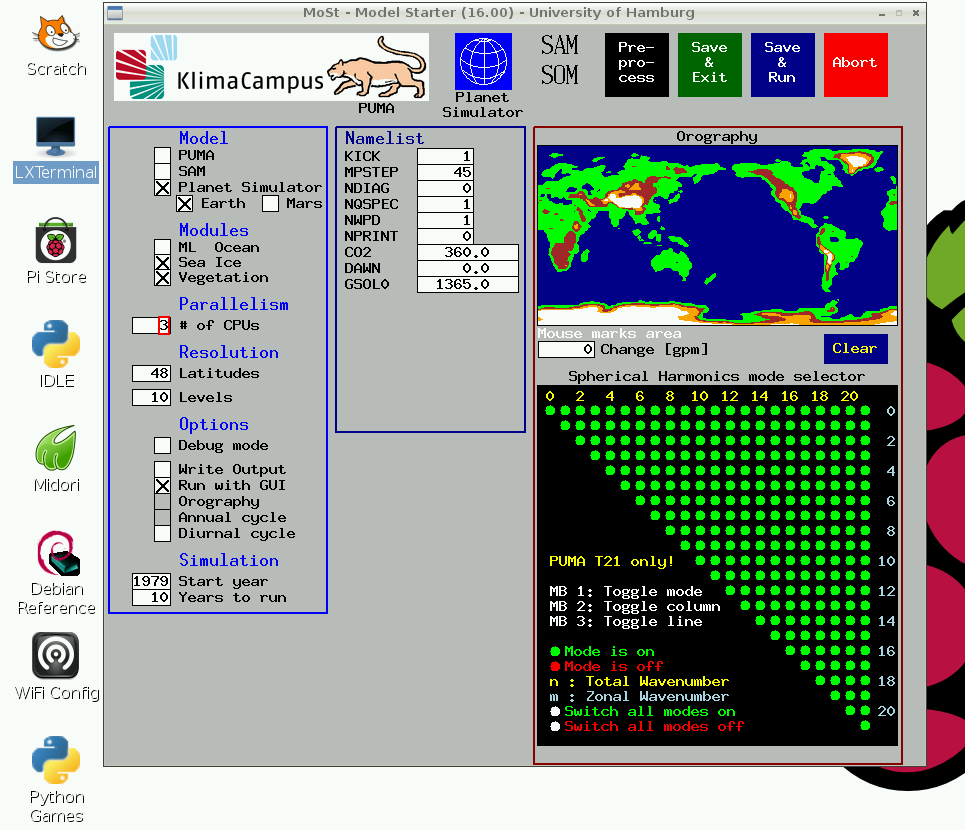
\includegraphics[height=12em]{Chapters/Chapter3/Figures/plasim-main}
	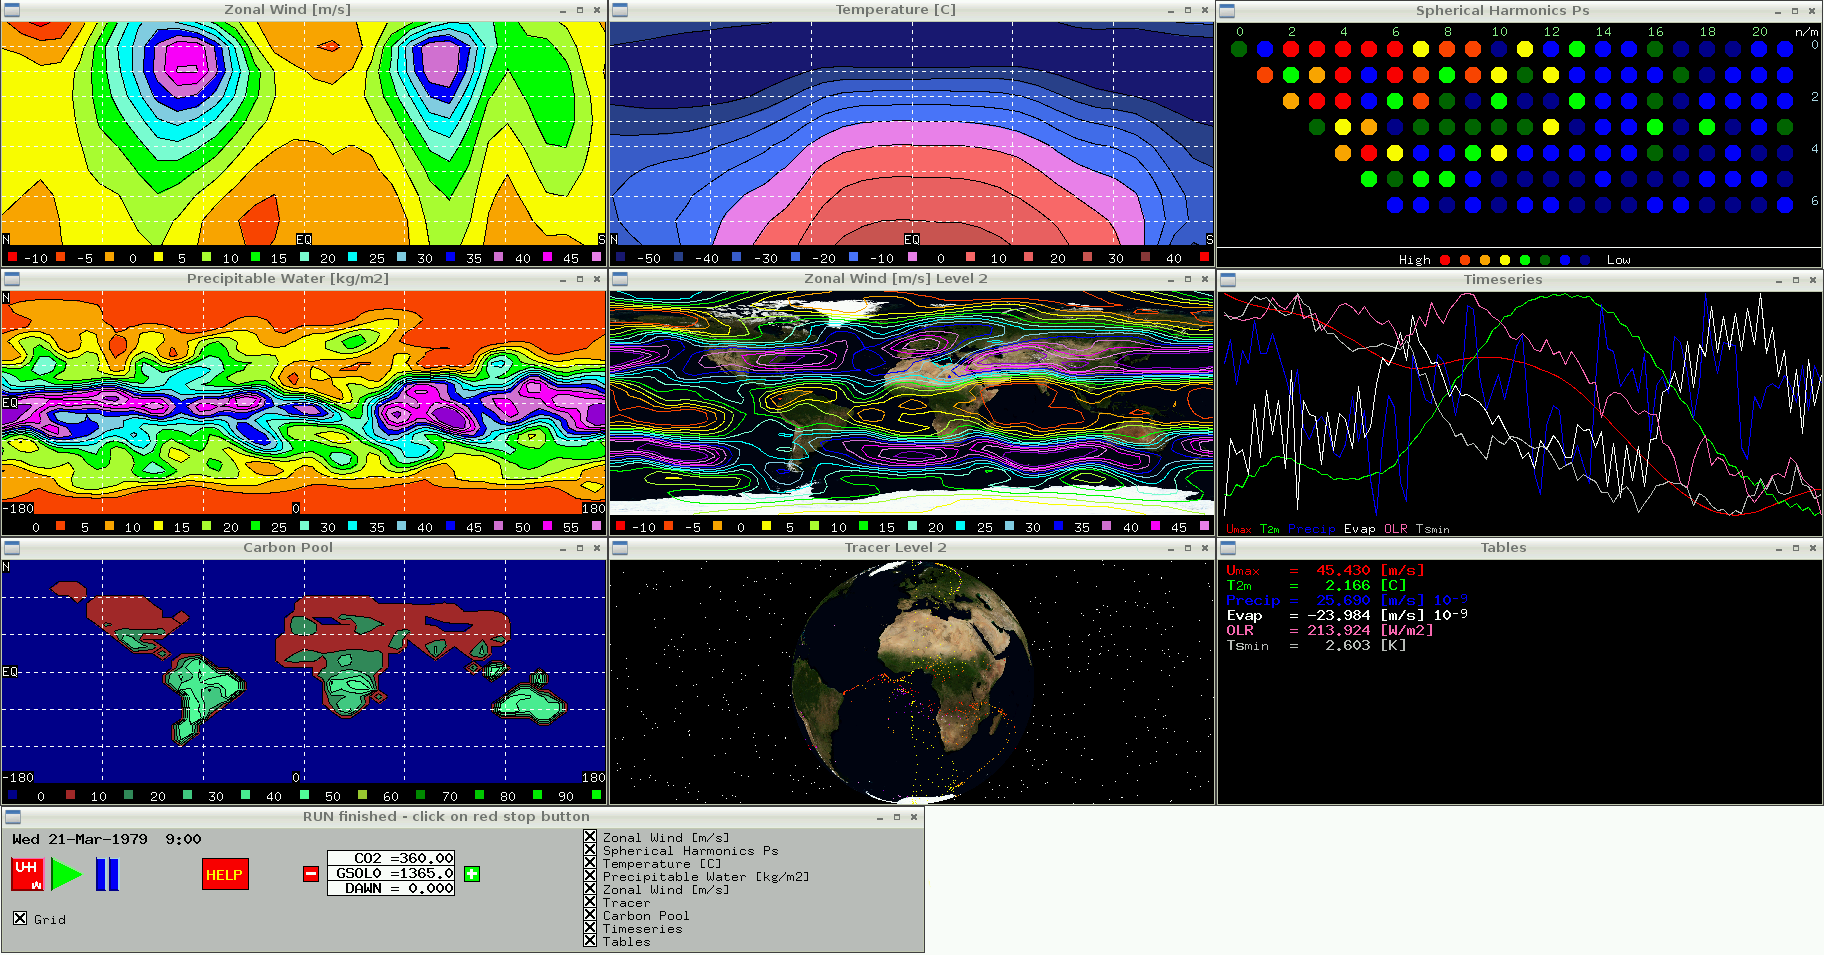
\includegraphics[height=12em]{Chapters/Chapter3/Figures/plasim-results}
	\label{fig:plasim}
	\caption[Interfaz de la aplicación \textit{Planet Simulator}]{Interfaz de control del \textit{Planet Simulator} y vista de ejecución de una simulación}
\end{figure}

Este proyecto ha sido evaluado con el objetivo de integrarlo en el sistema. Sin embargo, el programa depende considerablemente de la interfaz gráfica del mismo, inaccesible desde cualquiera de los nodos del sistema. A fin de solventar este problema se plantea el uso de un equipo de escritorio que cree los ficheros de configuración y los distribuya entre los nodos. Esta posibilidad se debe descartar finalmente, dado que el simulador realiza la compilación del programa con los parámetros fijados en la interfaz gráfica. Dado que los binarios creados para la arquitectura de un equipo de escritorio (x86, x86-64) son incompatibles con el \textit{hardware} de los nodos (arquitectura ARM) y hay tareas con mayor prioridad, se descarta esta tarea de forma indefinida, siendo finalmente no incluido en la versión final del sistema.

\subsection{Tomcat}

Las prácticas de la asignatura Sistemas Distribuidos se realizan sobre el contenedor de servicios Tomcat y el \textit{framework} Glassfish \footnote{\href{https://glassfish.java.net/}{https://glassfish.java.net/}} para la creación de APIs \textbf{REST}. Por ello el sistema ofrece instancias de Tomcat a todos los usuarios sin que estos deban realizar ningún tipo de configuración. Además, se habilita el uso de Tomcat en herramientas como \textbf{deployer} para facilitar el desarrollo de las prácticas.

Se plantea el análisis de alternativas para la creación de APIs \textbf{REST} como el \textit{framework} \textbf{Flask}.

\section{Herramientas de virtualización}

\subsection{QEMU}

QEMU\footnote{\href{http://qemu.org}{http://qemu.org}} es un emulador y virtualizador de código abierto compatible con un gran abanico de arquitecturas y sistemas operativos diferentes, siendo compatible con hipervisores como Xen o KVM. En el sistema se utiliza como la primera propuesta de optimización del rendimiento del sistema en tareas como la compilación de código fuente.

QEMU es popular a la hora de virtualizar instancias de sistemas operativos para la arquitectura ARM, y existe documentación sobre la virtualización de sistemas como \textbf{Raspbian} o \textbf{Arch Linux ARM}, por lo que no se realiza una evaluación de otras alternativas.

\section{Herramientas utilizadas para la gestión de código, calidad de \textit{software} y el proyecto}

\subsection{Git}

Git es un sistema de control de versiones capaz de gestionar proyectos de cualquier escala, diseñado para flujos de trabajo distribuidos. Git permite realizar operaciones de reversión de cambios, bifurcaciones y uniones de flujos de desarrollo y gestión de varias copias independientes sin conflictos. Es una de las herramientas de gestión de código más utilizadas, siendo diseñada originalmente para la coordinación en el desarrollo del núcleo Linux.

Las diferentes herramientas que componen el sistema son creadas en repositorios independientes de código. Dicho código es almacenado en un servidor con el objetivo de facilitar la movilidad del código entre las diferentes máquinas que componen el sistema y a modo de copia de seguridad. Se sigue un modelo de desarrollo basado en ramas que representan características a añadir a la versión estable, revisión de código, documentación o mantenimiento y solución a \textit{bugs}.

Todos los repositorios de código originales pueden consultarse en \ref{repositorios}.

Dado que se cuenta con bastante experiencia en el uso de \textbf{git} no se analizan alternativas como \textbf{subversion} o \textbf{mercurial}. 

\subsection{Redmine}

Redmine es una herramienta de gestión de proyectos basada en web que permite a un equipo mantener un registro de todo el trabajo realizado y planificado en un proyecto, con una serie de herramientas como diagramas de Gantt, Wiki o integración con sistemas de control de versiones.

El proyecto cuenta con una instancia de Redmine alojada en \href{http://redmine.martinarroyo.net/projects/tfg}{http://redmine.martinarroyo.net/projects/tfg}. En dicha instancia se han registrado todos los avances en el desarrollo del proyecto desde las fases iniciales del mismo.

\subsection{2to3, 3to2}

Las versiones del lenguaje Python 2 y 3 son incompatibles entre sí. Sin embargo, las diferencias entre ambas versiones radican en una serie de variaciones sintácticas, nombres de tipos y localización de las bibliotecas estándar, por lo que escribiendo código que tenga en cuenta dichas variaciones, bien incluyendo sentencias condicionales en función de la versión o bien escribiendo código ambivalente es posible generar código compatible.

2to3 y 3to2 son herramientas que ayudan al programador en la verificación de la compatibilidad entre versiones, generando una lista de modificaciones que posibilitan la ejecución el código en otra versión. Utilizando ambas herramientas es posible crear código ambivalente de forma sencilla. Existen además guías y otras herramientas que facilitan este objetivo\footnote{\href{https://docs.python.org/3/howto/pyporting.html}{https://docs.python.org/3/howto/pyporting.html}}.

\subsection{Pylint}

Pylint es una herramienta de verificación de código, que evalúa la calidad de un fichero siguiendo una serie de criterios tales como la presencia de errores sintácticos, sangrado del código, convenciones de nombrado y de estilo, errores en la importación de paquetes, etcétera. Pylint incluye además la herramienta \textbf{pyreverse}, útil en la generación de diagramas UML.

\subsection{Desarrollo dirigido por pruebas: Unittest, CppUnit, Trial}

Uno de los mecanismos para la detección temprana de errores es el desarrollo dirigido por pruebas (ver \ref{teoria:tdd}). En el proyecto se utilizan diferentes \textit{frameworks} para cada una de las aplicaciones y bibliotecas creadas. Los tests unitarios se incluyen en cada uno de los paquetes para poder ser ejecutados por cualquier usuario en caso de que lo estime oportuno.

\section{Herramientas de modelado}
\subsection{Visual Paradigm}

Junto a \textbf{pyreverse} se utiliza la aplicación Visual Paradigm durante las etapas de documentación y modelado de las diferentes aplicaciones, en concreto, las herramientas de creación de diagramas UML y su generación automática a través del análisis del código fuente.

\section{Herramientas utilizadas para la documentación del proyecto}

\subsection{{\LaTeX}}

El sistema de composición de textos {\LaTeX} es utilizado para crear todos los documentos incluidos en el desarrollo del sistema. Se utiliza el motor {\XeLaTeX} para el compilado de los ficheros, debido a su mayor variedad de fuentes y la utilización por defecto de la codificación UTF-8 (útil en idiomas que utilizan un alfabeto diferente al del inglés). 

Se utiliza {\BibTeX} como gestor de la bibliografía en todos los documentos producidos.

\subsection{Sphinx}

Sphinx es un sistema de creación y generación de documentación capaz de crear documentos en diferentes formatos (HTML, \LaTeX, ePub\dots) a partir de una serie de archivos en el formato reStructuredText. Es además capaz de crear documentación sobre código Python (lenguaje para el que la herramienta fue creada) a partir de los comentarios presentes en el código (conocidos como \textbf{docstrings}). Junto con Doxygen, se ha conseguido documentar código en C, C++, Java, bash y JavaScript. Soporta además referencias cruzadas a diferentes proyectos creados con esta herramienta, muy útil en este caso concreto, donde se cuenta con un número de documentos independientes muy alto que se referencian entre ellos.

Los resultados generados por la herramienta son incluidos como documentación técnica de cada una de las herramientas, y están disponibles en \href{marcopolo.martinarroyo.net}.

\subsection{Doxygen}

Doxygen es un sistema similar a Sphinx utilizado en proyectos escritos en C, C++ y Java entre otros muchos lenguajes. Constituye el estándar \textit{de facto} para la generación de documentación.

En el proyecto Doxygen es utilizado para documentar aquellas partes del proyecto que Sphinx no puede procesar (actualmente el soporte de dicha herramienta se limita a Python). Posteriormente la documentación de ambas herramientas se combina mediante ficheros XML generados por Doxygen que Sphinx puede procesar.

\section{Herramientas para la gestión de usuarios}

\subsection{PAM, LDAP}

La gestión de los usuarios está delegada al sistema de autenticación preexistente en la infraestructura en la que se integra el sistema. En ella se cuenta con un servidor \textbf{LDAP}\footnote{\href{ldap1.cie.aulas.usal.es}{ldap1.cie.aulas.usal.es}} con la información de los usuarios. Mediante la configuración del paquete \textbf{LDAP} es posible acceder a los mismos, y gracias a \textbf{PAM} (\textit{Pluggable Authentication Module}) se integra con el resto de métodos de autenticación presentes en el sistema.

Se ha creado un módulo para \textbf{PAM} para facilitar las tareas que el sistema debe realizar. Dicho módulo integra \textbf{MarcoPolo} y es conocido como \textbf{pam\_mkpolohomedir}\ref{pam_mkpolohomedir}.

\section{Herramientas para la optimización del rendimiento}

\subsection{Distcc}

Distcc\footnote{\href{https://code.google.com/p/distcc/}{https://code.google.com/p/distcc/}} es la herramienta utilizada para el desarrollo del compilador distribuido. Se basa en una arquitectura cliente-servidor donde los trabajos de compilación pueden ser repartidos entre varios servidores para reducir el tiempo total de compilación, implementando mecanismos de verificación y balance de carga.

Junto con \textbf{crosstool-ng} conforma el compilador distribuido del sistema (ver \ref{crosstool-ng}).

\subsection{SSH-HPN}
\label{ssh-hpn}
Una de las características de OpenSSH es la ejecución de todas las tareas en un único proceso y por tanto, en un único núcleo, constituyendo un cuello de botella que se hace notable en computadores de bajas prestaciones, como el sistema a modelar que sin embargo, cuentan con un procesador multinúcleo.

Con el objetivo de superar este límite nace SSH-HPN\footnote{\href{http://www.psc.edu/index.php/hpn-ssh}{http://www.psc.edu/index.php/hpn-ssh}}, un conjunto de modificaciones al código fuente de OpenSSH que optimiza la ejecución del mismo mediante el uso de diferentes procesos repartidos en los diferentes núcleos del sistema. El proyecto se distribuye como un archivo \texttt{.diff} que se incluye en los archivos del código fuente con la herramienta \textbf{GNU patch}.

Se ha creado una versión parcheada de SSH probada en la instalación de Arch Linux utilizada con el código fuente ya preparado para trabajar en la arquitectura ARM utilizándose en lugar del paquete \textbf{OpenSSH} original.

%TODO\section{Otras herramientas}

%TODOArchivo BibTeX con todas las referencias de las RFCs: \href{http://tm.uka.de/~bless/bibrfcindex.html}{http://tm.uka.de/~bless/bibrfcindex.html}

\section{Metodología de desarrollo}

Una metodología de desarrollo reúne el conjunto de procesos y técnicas que se emplean en la construcción de un producto \textit{software}. La metodología debe ser elegida cuidadosamente en virtud de los objetivos y restricciones del proyecto, pues tiene el potencial de condicionar su buen devenir o actuar en detrimento del mismo.

Existen diferentes metodologías que satisfacen un conjunto diferente de demandas y son aptas para un tipo de proyecto, como el Proceso Unificado (cíclico, conducido por casos de uso), procesos ágiles (desarrollo incremental, tolerancia a cambios inesperados) o los modelos tradicionales (modelo lineal, en V, orientado a prototipos\dots).

En el caso del presente proyecto, se debe construir un conjunto de herramientas \textit{software} sin contar con abundante experiencia en el desarrollo de sistemas de este tipo, por lo que el grado de incertidumbre es muy alto. Es por ello que la metodología elegida debe ser capaz de lidiar con situaciones difíciles de predecir, cambios continuos en los requisitos definidos y poder responder ante problemas como la inviabilidad de una propuesta de solución, detectando dicha circunstancia de forma prematura. Se apuesta por un modelo ágil apoyado en prototipos, descrito en \ref{process}.
 % Técnicas y herramientas

\lhead{\emph{Dominio del problema}}
\chapter{Dominio del problema}

La utilización de algoritmos distribuidos implica mejoras sustanciales en una gran cantidad de aplicaciones, incrementando la capacidad global de cómputo de un sistema mediante la unión de varios dispositivos que trabajan como una única unidad manteniendo simultáneamente un alto grado de independencia y una tolerancia global a fallos muy alta. Sin embargo, el coste de la adquisición instalación y mantenimiento de dicho conjunto de nodos suele ser elevado. Además, los beneficios citados implican una mayor complejidad en el desarrollo de algoritmos que puedan aprovechar de forma óptima este tipo de sistemas. Varios factores como la sincronización y la comunicación entre partes, o errores tales como condiciones de carrera son mucho más comunes que en otro tipo de aplicaciones. Dichas circunstancias no solo dificultan el desarrollo de este sistema, sino también la comprensión de los fundamentos básicos de la Computación Distribuida, aspecto de relevancia para estudiantes de Ciencias de la Computación.

Si bien la mayoría de las aplicaciones en las que el paradigma de computación distribuida introduce mejoras suelen exigir una gran capacidad de cálculo, su desarrollo únicamente requiere un conjunto de instancias independientes de un \textit{software} (sistema operativo, contenedor de servicios\dots) con las que trabajar. Dicha característica implica que la utilización de nodos de precio reducido (o incluso equipos ya presentes en una infraestructura) para el diseño, análisis y evaluación de este tipo de algoritmos constituye una alternativa válida frente a sistemas de precio superior.

Sumada a dicha motivación existe el potencial aprovechamiento de este sistema como herramienta didáctica que facilite el aprendizaje de conceptos como el reparto de procesos, balance de carga o la compartición de recursos en asignaturas centradas en este tipo de conceptos dentro de los planes de estudio de Ingeniería Informática o titulaciones similares.

En el presente proyecto se realiza un análisis de las diferentes alternativas que permitan satisfacer los objetivos definidos previamente.

%TODOFigura: Tabla de alternativas

\section{Definiciones}

\subsection{Definición del dominio del problema}

%TODO

\subsection{Sistema actual: Infraestructura de la Facultad de Ciencias}
\label{dominioproblema:infraestructura}
El sistema se ubica en una Facultad universitaria con 1.463 alumnos\cite{uecusal:estudiantes} en titulaciones relacionadas con las Ciencias de la Computación. Estas titulaciones cuentan con varias asignaturas relacionadas con el áreas de conocimiento Computación Distribuida, en particular \textbf{Arquitectura de Computadores} y \textbf{Sistemas Distribuidos} \cite{DIA15GuiaAcademica}. La Facultad cuenta con varias aulas y laboratorios de informática donde los alumnos disponen de la infraestructura necesaria para realizar los ejercicios y prácticas asignadas. Dichos espacios permiten utilizar cualquier equipo como nodo, pues se integran en la misma red, siendo incluso factible la comunicación directa entre equipos situados en diferentes aulas o incluso edificios. Todos los edificios cuentan con un cableado capaz de soportar teóricamente transferencias de hasta 100 Mb/s de forma bidireccional. La gestión de un sistema de autenticación se realiza mediante el protocolo \textbf{LDAP} (\textit{Lightweight Directory Access Protocol})\cite{RFC4516-comment}, contando con un sistema de ficheros centralizado que permite acceder a la información de un usuario desde cualquier equipo, facilitando las tareas de replicación de la información entre nodos\footnote{Datos extraídos de entrevistas con el Administrador de la infraestructura}.

La mayoría de las prácticas asignadas a los alumnos en las asignaturas de interés son desarrolladas en los lenguajes de programación \textbf{C} y \textbf{Java}, ya conocidos por la totalidad de los estudiantes gracias a asignaturas previamente cursadas.

\paragraph{Problemas conocidos}

Si bien la infraestructura existente es capaz de proveer a los estudiantes de los recursos necesarios, se identifican una serie de problemas inicialmente:

\begin{itemize}
  \item Cada grupo de alumnos necesita tres estaciones de trabajo para poder realizar algunos de los ejercicios propuestos.
  \item El servidor \textbf{LDAP} constituye un ``cuello de botella'', pues todos los alumnos acceden a él de forma intensiva, provocando el fallo por exceso de peticiones del mismo.
  %TODO\item Las técnicas de programación utilizadas hasta la fecha tienen un rendimiento bajo y son en ocasiones relativamente complejas.
\end{itemize}

\subsubsection{Análisis de estadísticas}
\label{dominio:estadisticast}
%Pandora magic

\section{Identificación de \textit{stakeholders}}

Un \textit{stakeholder} es cualquier grupo o individuo que tiene es afectado o afecta a la consecución de los objetivos de un proyecto marcados por una organización, así como un particular interés en el devenir del mismo. Claros ejemplos de este tipo de entidades son los diferentes usuarios finales del sistema, potenciales clientes o el equipo de desarrollo, entre muchos otros.

En el proyecto en cuestión se identifican los siguientes \textit{stakeholders} y su motivación.

\begin{itemize}
  \item Equipo de desarrollo. Su motivación es la consecución de todos los objetivos marcados en el sistema.
  \item Estudiantes de tercer y cuarto curso del Grado en Ingeniería Informática, que podrán utilizar el sistema como herramienta didáctica.
  \item Profesores de las asignaturas Arquitectura de Computadores y Sistemas Distribuidos, que aprovecharán el sistema final en dichas asignaturas.
  \item Administradores del sistema, que deberán hacerse cargo del mantenimiento del sistema a largo plazo.
\end{itemize}

\subsection{Identificación de las necesidades de cada parte}

Basándose en la motivación de cada parte es posible definir las demandas de cada una de las partes. Otros mecanismos, como la realización de entrevistas u observaciones permiten complementan dicho proceso.

\subsubsection{Alumnos}

\begin{itemize}
  \item Entorno de trabajo intuitivo y documentado que agilice el desarrollo de sus prácticas.
  \item Posibilidad de observar los resultados de las ejecuciones de forma sencilla.
  \item Depuración sencilla.
  \item Facilidades para el despliegue de los diferentes ejecutables en todas las máquinas, así como el consumo de los servicios que estos implementen.
\end{itemize}

\subsection{Necesidades de los docentes}

\begin{itemize}
  \item Entorno versátil sobre el cual puedan llevarse a cabo la totalidad de las prácticas y ejercicios propuestos, aportando si es posible algún tipo de ventaja sobre el sistema en uso.
  \item Instalación y configuración simple.
\end{itemize}

\subsection{Administradores}

\begin{itemize}
  \item Sistema integrable en la infraestructura actual cuyo mantenimiento sea sencillo y cuyo enfoque garantice la escalabilidad y su durabilidad. Documentación extensa sobre el funcionamiento interno del sistema.
  \item Instalación y configuración simple.
  \item Mantenimiento sencillo.
\end{itemize}

\section{Propuestas para la búsqueda de necesidades}

\begin{itemize}
  \item Encuestas o entrevistas a todas las partes.
  \item Observación.
  \item Evaluación de la experiencia de uso en las diferentes etapas de desarrollo del sistema.
\end{itemize}

\section{Identificación de requisitos}

\subsection{Requisitos de almacenamiento de la información}

\begin{itemize}
  \item Gestión de usuarios (credenciales de autenticación).
  \item Gestión de los datos de cada usuario.
  \item \textit{Logs} del sistema
  \item Ficheros de configuración, bases de datos de gestión\dots
\end{itemize}

\subsection{Identificación de requisitos funcionales}


\subsection{Identificación de requisitos no funcionales}

\subsubsection{Mantenimiento y robustez}

El \textit{software} debe ser mantenible y robusto, siendo dicha robustez garantizada mediante el uso de \textit{software} utilizado por una base de usuarios significativa, una arquitectura conocida, pruebas realizadas sobre él o un equipo de desarrollo en activo, entre otras.

\subsubsection{Costes de desarrollo}

El coste de desarrollo no debe superar un total de 400 €.

\subsubsection{Definición de los protocolos de comunicación}

Los diferentes protocolos utilizados o creados para el sistema deben ser públicos y extensibles a diferentes paradigmas de utilización y tecnologías que los implementen.

\subsubsection{Definición de los protocolos de seguridad y confidencialidad}

Se utilizará una infraestructura de clave pública para la mayoría de las transacciones cifradas realizadas en el sistema.

\subsubsection{Definición de la interacción con el usuario}

Todos los mecanismos de interacción con el usuario deberán definirse de forma precisa.

\subsubsection{Integridad del sistema y fiabilidad (\textit{uptime}, recuperación frente a fallos)}

\subsubsection{Compatibilidad con prácticas y otros ejercicios}

El sistema deberá ser compatible los ejercicios desarrollados en las asignaturas \textbf{Arquitectura de Computadores} y en especial \textbf{Sistemas distribuidos}

\section{Situación actual (\textit{state of the art})}
\label{stateoftheart}
En esta sección se definen diferentes enfoques ya aplicados a soluciones a problemas similares al planteado anteriormente.

\subsection{Computadores de placa única}

El uso de computadores de prestaciones reducidas como componentes de un sistema distribuido ha experimentado un gran crecimiento en los últimos años debido a la popularización y el abaratamiento de este tipo de dispositivos, existiendo gran cantidad de fabricantes y proveedores de \textit{software} para los mismos.

Los computadores de placa única (\textit{Single-Board Computers}) son máquinas de generalmente bajas prestaciones que aglutinan todos los componentes necesarios para su funcionamiento en un único circuito impreso. Suelen tener un coste bajo y una relación rendimiento/coste elevada. Su versatilidad y precio reducido han propiciado su uso como herramienta para el estudio y creación de sistemas distribuidos con un gran rango de propósitos diferentes.

\subsubsection{RPiCluster (Joshua Kiepert)}

Joshua Kiepert, estudiante de doctorado en la universidad Boise State, crea este sistema utilizando 33 computadores \textbf{Raspberry Pi B}, con el objetivo de utilizarlo como herramienta de pruebas que sirva de alternativa al supercomputador con el que su universidad cuenta\cite{joshuarpicluster} y sobre el que trabaja de forma rutinaria, con el objetivo de poder continuar su trabajo en periodos de mantenimiento, cierre del centro, etcétera. El sistema está diseñado para utilizar la \textit{Message Passing Interface} como mecanismo de comunicación y coordinación (siguiendo un esquema maestro-esclavo) y además utilizar los diferentes puertos de las placas (GPIO, I\textsuperscript{2}C, SPI, UART), puertos generalmente ausentes en computadores convencionales. Utiliza además un sistema \textbf{NFS} (\textit{Network File Storage}) para compartir datos entre todos los nodos, y un \textit{router} dedicado para la interconexión. El sistema se completa con un ordenador portátil \textbf{Chromebook} con el mismo sistema operativo que los nodos del sistema, (\textbf{Arch Linux}), que actúa como nodo coordinador. La estructura incluye el conjunto de nodos esclavos y coordinador, dos fuentes de alimentación y un mecanismo de refrigeración, así como un mecanismo de distribución de la energía (diseñado por Kiepert) y de gestión de los diodos LED que incluye cada nodo y que son utilizados como elemento estético y mecanismo de análisis visual del comportamiento de los algoritmos ejecutados\footnote{Vídeo del sistema en ejecución: \href{https://www.youtube.com/watch?v=i_r3z1jYHAc}{youtube.com/watch?v=i\_r3z1jYHAc}}.

%TODO: http://www.zdnet.com/article/build-your-own-supercomputer-out-of-raspberry-pi-boards/

\begin{figure}[H]
  \centering
  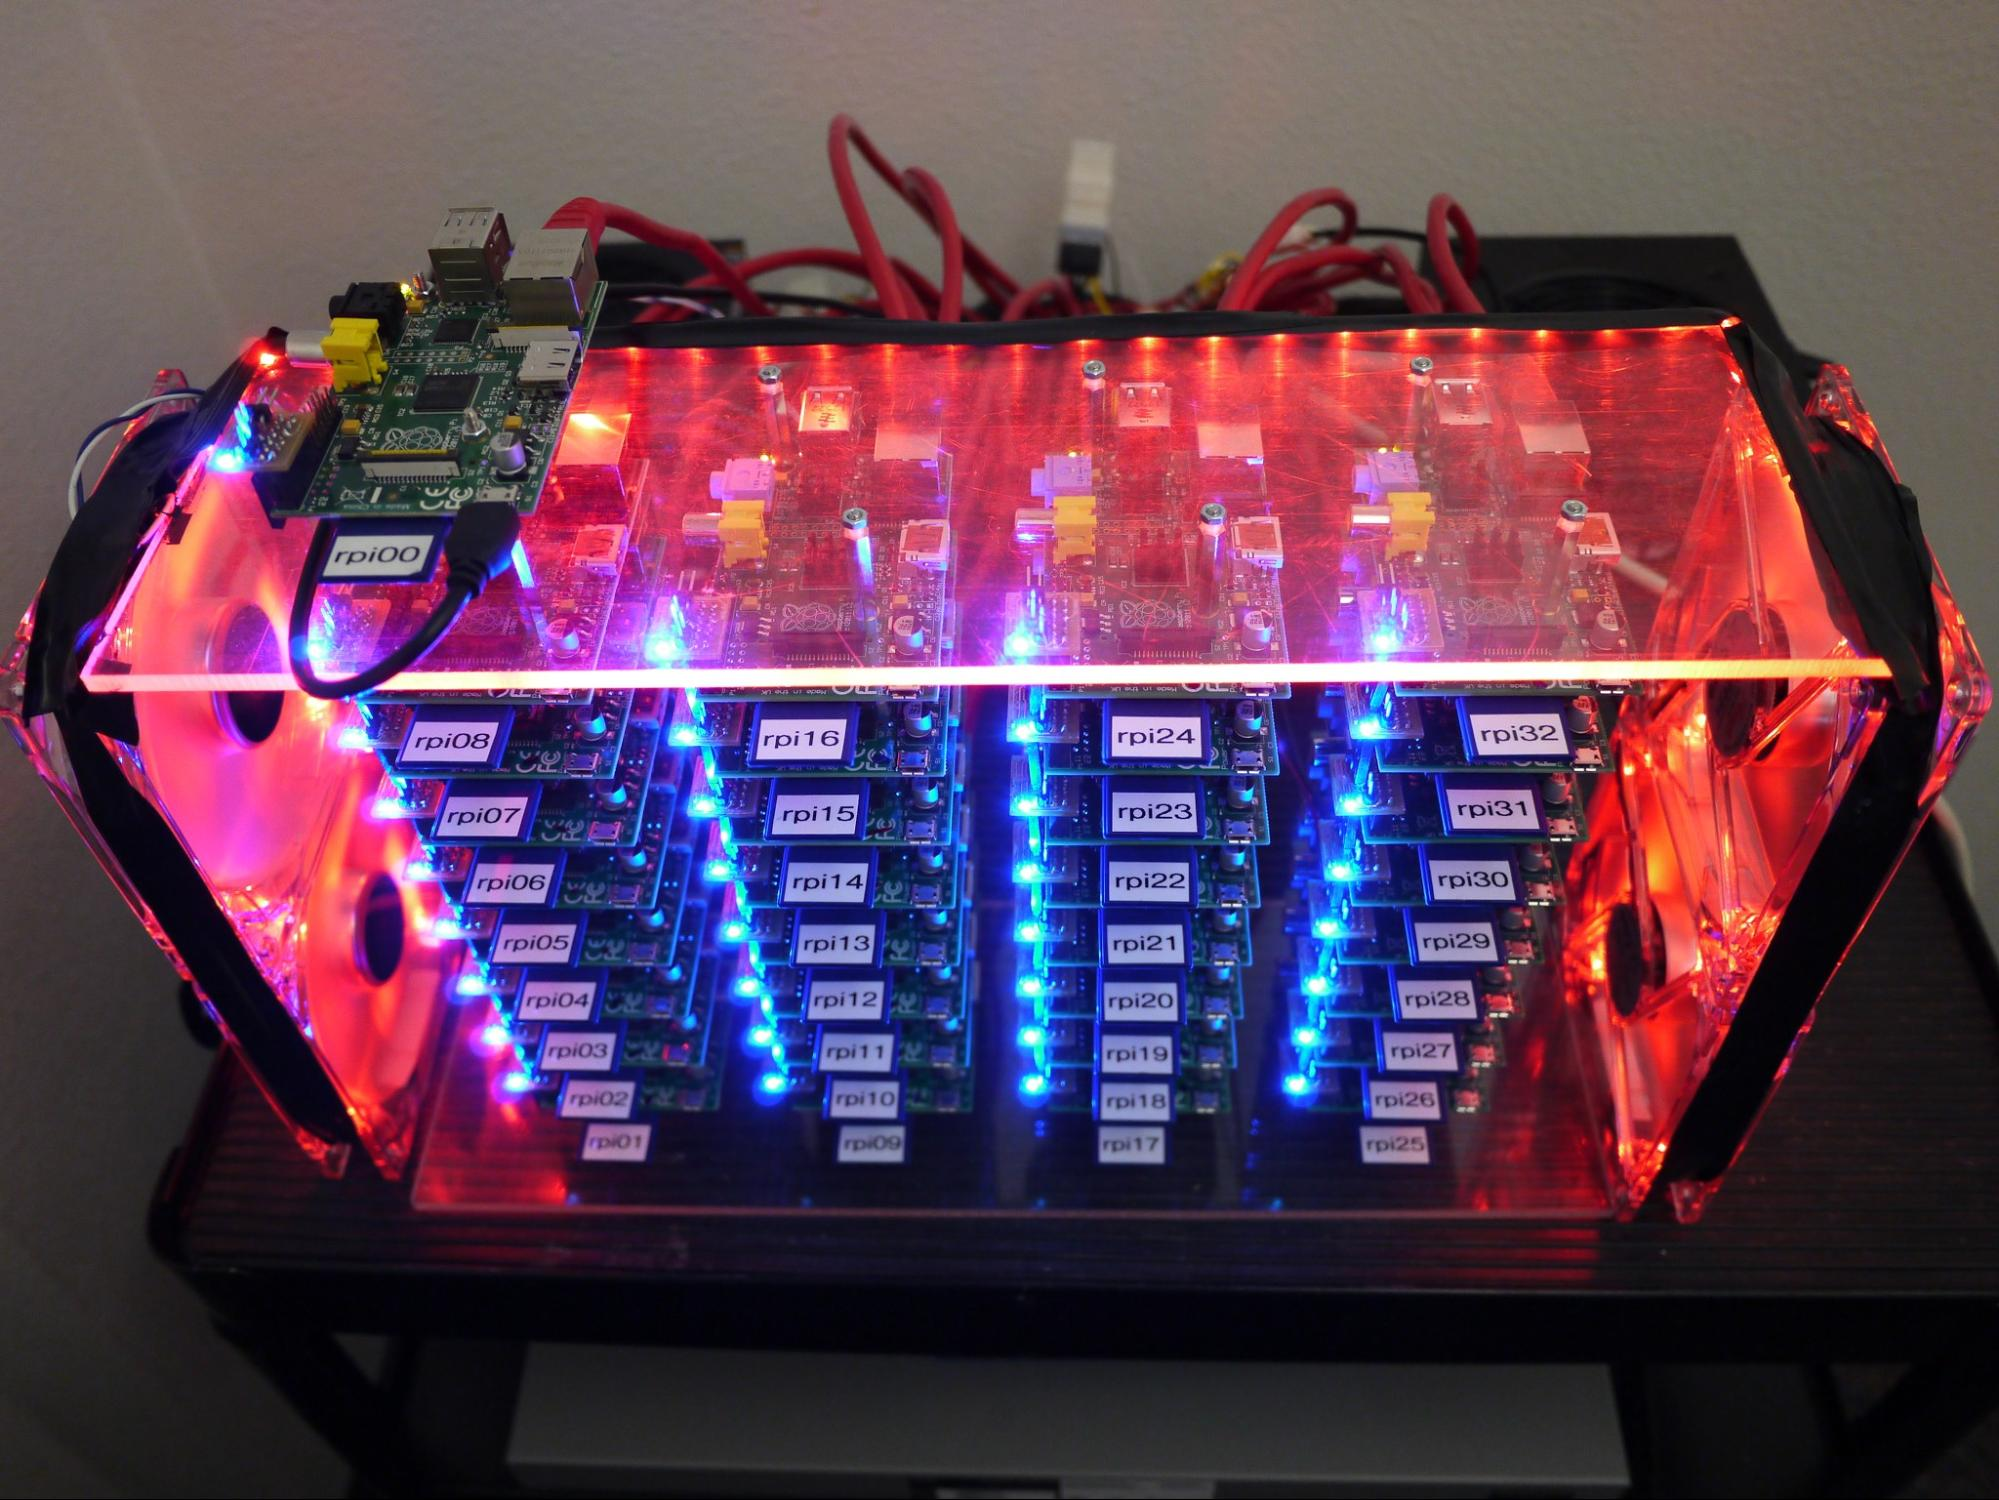
\includegraphics[width=0.36\textwidth]{Chapter4/Figures/kiepert-main}
  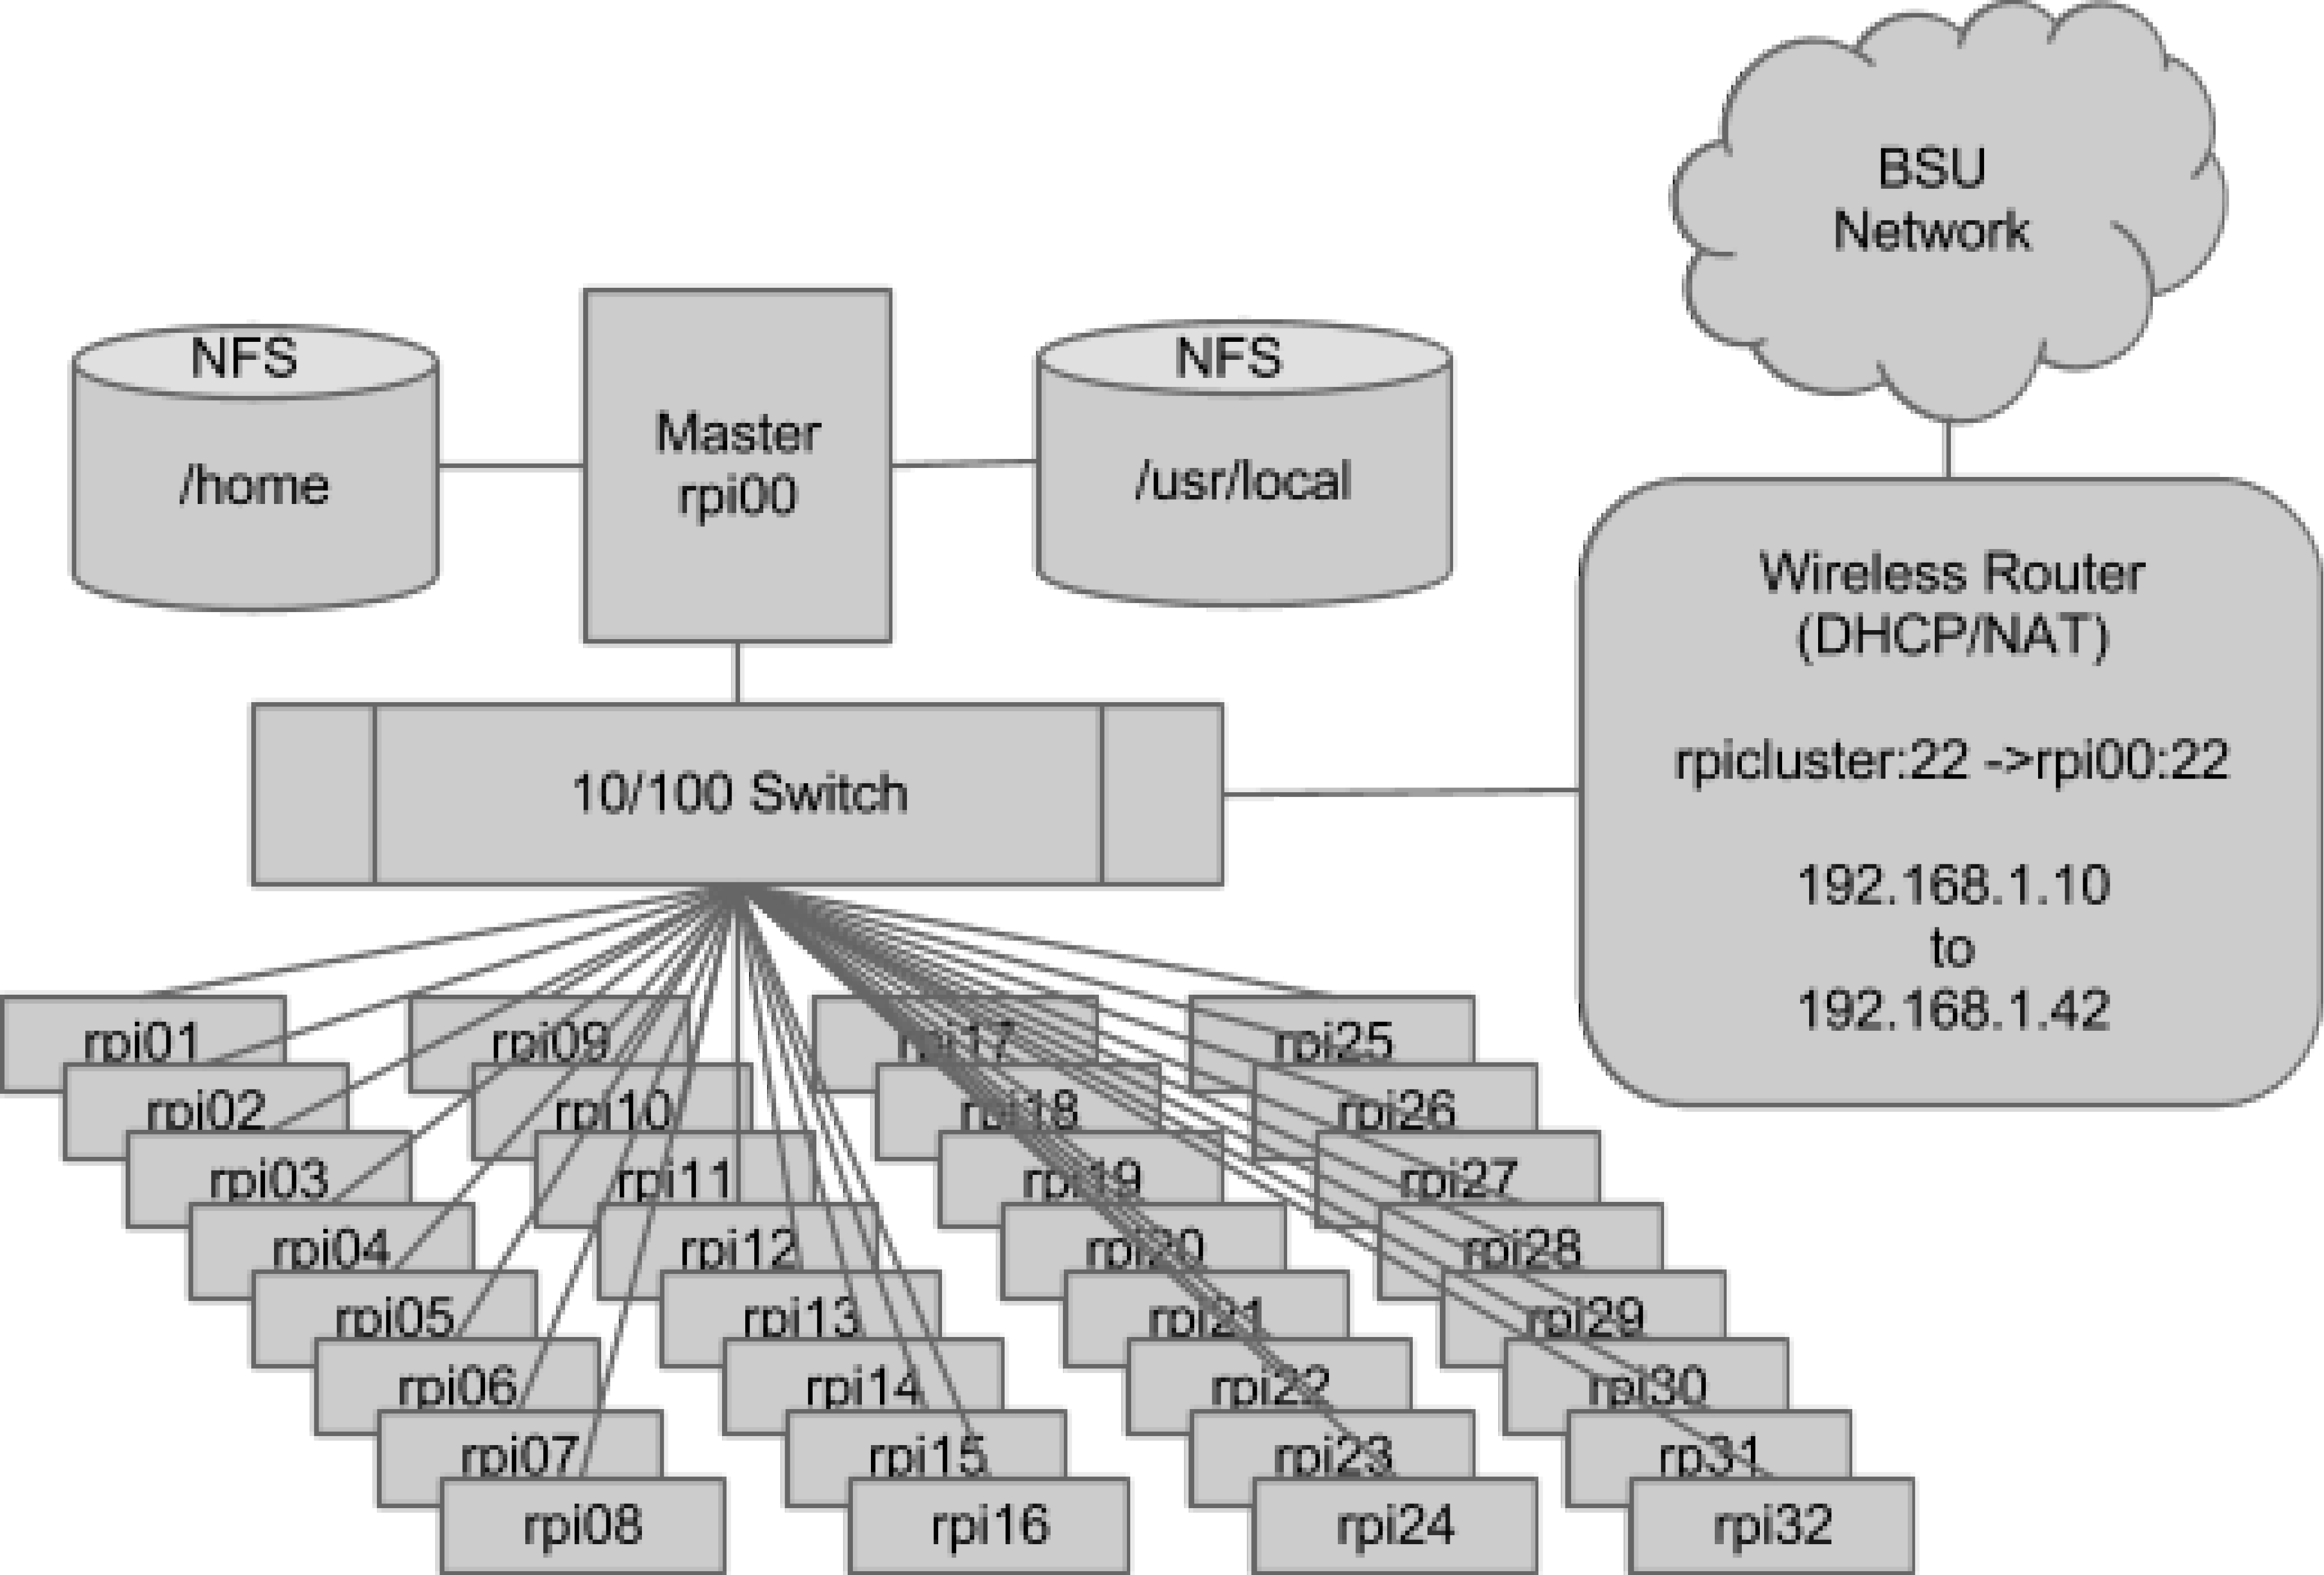
\includegraphics[width=0.4\textwidth]{Chapter4/Figures/kiepert.png}
  \caption[RPiCluster]{Vista general y estructura del sistema (Fuente: Joshua Kiepert)}
  \label{kiepert:structure}
\end{figure}

El coste total del proyecto según Kiepert es de 1967.21 dólares.

\subsubsection{Dramble (Jeff Geerling)}

El clúster \textit{Dramble} está formado por 6 equipos \textbf{Raspberry Pi} capaces de ejecutar en conjunto el gestor de contenidos \textbf{Drupal}\footnote{\href{https://www.drupal.org/}{drupal.org}}. Es utilizado como servidor de pruebas para la ejecución de instancias de este \textit{software} de forma experimental o durante demostraciones en público\cite{geerlingraspberry}. Se compone del conjunto de nodos \textit{Rasbperry Pi} y los mecanismos de red y alimentación que interconectan y proveen de energía a los mismos.

\begin{figure}[H]
  \centering
  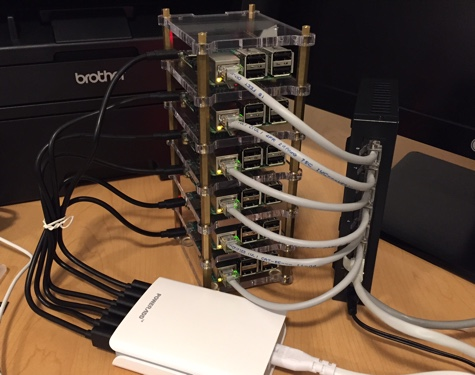
\includegraphics[width=0.5\textwidth]{Chapters/Chapter4/Figures/raspberry-pi-dramble-cluster-wired.jpg}
  \caption[Dramble]{El \textit{Dramble} en ejecución}
  \label{geerling:dramble}
\end{figure}

El coste estimado es de 35 dólares por cada Raspberry Pi mas el coste añadido de la red y el cableado de alimentación, totalizando aproximadamente 300 dólares.

\subsection{Bramble (GCHQ)}

El organismo gubernamental \textit{Government Communication Headquarters}, agencia de inteligencia del Gobierno Británico presentó en la \textit{Big Bang Fair} de 2015 un proyecto educativo que combina 66 \textit{Raspberry Pi} en un clúster jerárquico con 8 grupos de 8 nodos, cada uno de ellos con un coordinador. El cableado se reduce gracias al uso de la tecnología \textbf{PoE} (\textit{Power over Ethernet}), y cada \textbf{Raspberry} cuenta con un conjunto de elementos adicionales, como un reloj de tiempo real, disco duro externo, cámara, o punto de acceso WiFi\cite{gchqbramble}.

\begin{figure}[H]
  \centering
  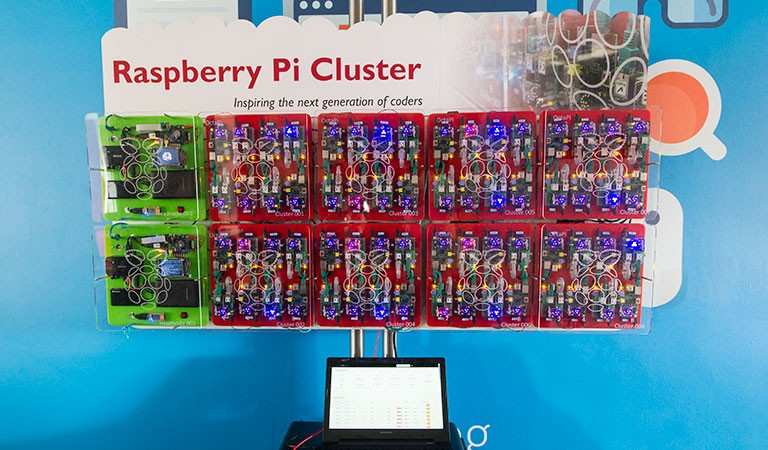
\includegraphics[width=0.8\textwidth]{Chapters/Chapter4/Figures/bramblegchq}
  \caption[Bramble]{Vistazo general de la estructura del sistema Bramble}
  \label{gchq:bramble}
\end{figure}

Se desconocen datos sobre el coste total del sistema.

\subsection{Clúster Iridis (Simon Cox, University of Southampton)}

Con el objetivo de atraer a jóvenes estudiantes al mundo de la computación, el profesor Simon Cox crea este clúster con 64 \textbf{Raspberry Pi B} sobre una estructura construida con LEGO\cite{cox:raspberry}. El sistema está diseñado para ejecutar aplicaciones sobre \textit{MPI}. Se desconocen datos sobre el coste total del sistema.

\begin{figure}[H]
  \centering
  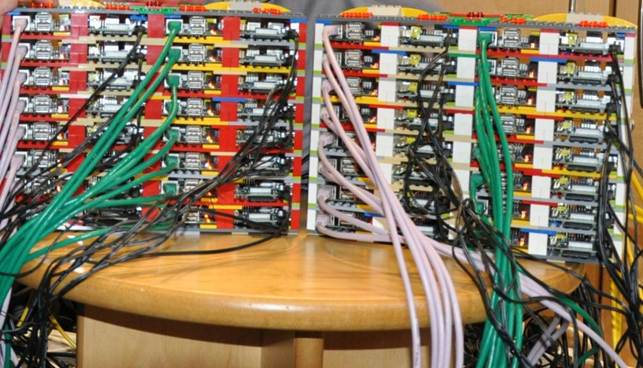
\includegraphics[width=0.65\textwidth]{Chapters/Chapter4/Figures/iridis-pi.jpg}
  \caption[Iridis]{Clúster Iridis}
  \label{cox:iridis}
\end{figure}

\subsection{Paralella}

Paralella es un proyecto de la compañía Adapteva que integra en un único chip un conjunto elevado de procesadores independientes con el objetivo de incrementar la capacidad de procesamiento total del sistema a un coste muy reducido\cite{paralella}. El coste es de 99 dólares por unidad.

\subsection{Virtualización}

Uno de los mecanismos para crear sistemas distribuidos en auge es la utilización de mecanismos de virtualización (ver \ref{teoria:virtualizacion}, que evitan el uso de diferentes unidades de \textit{hardware}. Estas soluciones se han popularizado en los últimos años principalmente en entornos empresariales, existiendo gran cantidad de proveedores de servicios y herramientas para la creación de un sistema propio (ver \ref{teoria:virtualizacion}). Ejemplos de este tipo de proveedores son \textbf{Amazon Web Services}\footnote{\href{http://aws.amazon.com/}{https://aws.amazon.com}}, \textbf{Google App Engine}\footnote{\href{https://cloud.google.com/appengine/}{https://cloud.google.com/appengine/}}, \textbf{Microsoft Azure}\footnote{\href{http://azure.microsoft.com/}{http://azure.microsoft.com/en-us/}} o \textbf{Digital Ocean}\footnote{\href{http://digitalocean.com}{http://digitalocean.com}}, entre muchos otros. Su éxito reside en su gran versatilidad: es sencillo crear y destruir nuevas réplicas de un sistema bajo demanda, ahorrando costes de forma significativa.

\subsection{\textit{Commercial Off-The-Shelf hardware}}

Este tipo de hardware está constituido por equipos disponibles al público de forma inmediata (\textit{off the shelf}) y generalmente son máquinas de propósito general, las cuales son interconectadas para crear un sistema distribuido que sirva de alternativa a utilidades más potentes, pero de coste superior (como un \textit{mainframe} o un ordenador de mayor potencia). Su coste económico (que se reduce si existe la posibilidad de aprovechar \textit{hardware} existente en la organización, como equipos de escritorio que no están en uso) es su mayor atractivo.

Un ejemplo de este tipo de sistemas son los clústeres \textit{Beowulf}\cite{beowulf:icpp95}, que se construyen sobre una red de área local y un sistema de intercomunicación como \textbf{MPI}, \textbf{PVM} u \textbf{OpenMP}. Existe gran cantidad de documentación para la creación de un clúster de este tipo\footnote{\href{http://tldp.org/HOWTO/Beowulf-HOWTO/}{tldp.org/HOWTO/Beowulf-HOWTO/}}, así como una serie de recursos (sistemas operativos, herramientas\dots) diseñadas con el propósito específico de crear este tipo de sistemas.


\section{Evaluación de alternativas}
\label{alternativas}
A la hora de evaluar las diferentes opciones que satisfagan los requisitos descritos, se consideran los siguientes aspectos:

\begin{itemize}
  \item Coste económico.
  \item Prestaciones técnicas (potencia de procesamiento, entrada/salida, capacidad de almacenamiento,facilidad de interconexión con otros elementos\dots).
  \item Facilidad de trabajo y de aprendizaje (documentación disponible, proyectos similares ya realizados, conocimiento previo sobre la plataforma en cuestión\dots).
  \item Escalabilidad del sistema.
  \item Necesidades de mantenimiento del sistema.
  \item Consumo eléctrico.
  \item Obsolescencia del sistema (periodo de tiempo en el que el \textit{hardware} y \textit{software} del sistema podrán ser actualizados y ser capaces de satisfacer los requisitos para los que fue creado).
\end{itemize}

\begin{comment}
% \subsection{Propuesta de solución: Virtualización de entornos de trabajo}

% Crear un conjunto de nodos virtuales dentro de una máquina que simulen un sistema distribuido

% \paragraph{Ventajas intrínsecas de la solución\\}

% Simplificación del sistema (reduce las necesidades de adquisición y mantenimiento de hardware).
% Gestión de varias partes del sistema (sistema de ficheros centralizado, gestión de usuarios\dots) de forma mas sencilla. El coste se reduce significativamente.

% \paragraph{Inconvenientes intrínsecos del sistema\\}

% No se exploran apenas las posibilidades de un sistema distribuido formado por varios equipos físicamente independientes e impide aprovechar dicha independencia para los objetivos didácticos del sistema.

% \paragraph{Facilidad de trabajo y curva de aprendizaje\\}

% Si bien el trabajo con cada una de las instancias es previsiblemente sencillo, debido a la eliminación de la gran parte del mantenimiento de la capa física subyacente, el uso de este tipo de sistema requiere una etapa de formación previa en materia de virtualización.

% \paragraph{Prestaciones técnicas\\}

% Las prestaciones técnicas con las que se contaría, de llevarse a cabo este proyecto, son las de los equipos ya dispuestos para fines similares a este en el Centro\citationneeded[Preguntar a Andrés]{}.

% \paragraph{Coste económico\\}

% El coste económico es muy reducido si ya se cuenta con los equipos a utilizar y las licencias del \textit{software} de virtualización necesarias.

% \paragraph{Escalabilidad del sistema\\}

% Dependiente de las capacidades de virtualización del equipo disponible, y el número de nodos y usuarios a gestionar.

% \paragraph{Necesidades de mantenimiento\\}

% Las necesidades propias de un sistema operativo multiusuario (previsiblemente \textbf{GNU/Linux}) junto a las específicas de la virtualización de los equipos (monitor de máquinas virtuales).

% \paragraph{Consumo energético del sistema\\}

% \citationneeded[Preguntar a Andrés]{}

% \paragraph{Obsolescencia del sistema\\}

% Se estima una larga vida útil del sistema. Las máquinas virtuales instaladas en un sistema físico son fácilmente trasladables a otro equipo, por lo que la dependencia de la parte física del sistema es muy baja.

% \paragraph{Material con el que se cuenta actualmente\\}

% Se plantea el aprovechamiento de equipos ya presentes en la infraestructura en la que trabajar, por lo que se estima un coste muy pequeño a la hora de adquirir material.

% \paragraph{Prestaciones técnicas\\}

% \citationneeded[Preguntar a Andrés]{}

% \paragraph{Análisis coste/beneficio\\}

% Si bien el coste de esta solución es muy atractivo, presenta una serie de carencias que dificultan significativamente el desarrollo del sistema en el mismo. 


% \subsection{Propuesta de solución: Clúster con equipos de escritorio}

% Se plantea la reutilización de equipos de escritorio pertenecientes a la Universidad que ya no se encuentran en uso (debido a su renovación, falta de potencia como PC\dots) para la creación de este sistema.

% \paragraph{Ventajas intrínsecas de la solución\\}

% La potencia del sistema es mucho mayor que la de cualquier otra solución considerada. Se reduce dramáticamente el coste de adquisición de material y permite dar un nuevo ciclo de vida a material universitario. La arquitectura es conocida y fiable.

% \paragraph{Inconvenientes intrínsecos del sistema\\}

% No se exploran las características únicas de otros sistemas menos ``convencionales'', como los sistemas embebidos. El consumo energético es mayor y existe una mayor demanda de espacio que puede dificultar la implementación de diferentes aplicaciones didácticas ya planteadas como objetivo funcional del sistema.

% \paragraph{Facilidad de trabajo y curva de aprendizaje\\}

% Soporte completo de casi la totalidad de las distribuciones de GNU/Linux. Las necesidades de manipulación de hardware se minimizan.

% \paragraph{Prestaciones técnicas}
% \begin{itemize}
%   \item Arquitectura x86/x86-64 (dependiendo de los equipos a utilizar finalmente).
%   \item Entre 2 y 4 GB de memoria principal.
%   \item Conectividad Ethernet, USB.
%   \item Almacenamiento en disco duro.
% \end{itemize}

% \paragraph{Coste económico\\}

% El coste económico de estos equipos es prácticamente nulo, pues ya se cuenta con los mismos y su utilización no exige la adquisición de nuevos equipos que los sustituyan. Estos equipos ya han sido retirados y no están empleados actualmente en ninguna tarea.

% \paragraph{Escalabilidad del sistema\\}

% Dependiente únicamente del coste económico de la adquisición de nuevos equipos, o de la disponibilidad de equipos que no estén utilizados.

% \paragraph{Necesidades de mantenimiento\\}

% Las propias de cualquier sistema multiusuario y las específicas del montaje dado (en materia de refrigeración, gestión de cableado, etcétera).

% \paragraph{Consumo energético del sistema\\}

% El típico de cualquier equipo de escritorio.

% \paragraph{Obsolescencia del sistema\\}

% Estos equipos tienen una antigüedad de aproximadamente 4 años. Dicha edad no impide que sean capaces de utilizar aplicaciones actuales, y en general no se prevé la incompatibilidad con ninguna aplicación. No obstante, son equipos relativamente antiguos que han sido utilizados de forma intensiva, por lo que la probabilidad de fallo en los mismos puede ser elevada.

% \paragraph{Material con el que se cuenta actualmente\\}

% Se cuenta con un número suficiente de equipos para la creación del sistema final.

% \paragraph{Análisis coste/beneficio\\}

% Si bien el coste de estos equipos es prácticamente nulo, dicho atractivo contrasta con los potenciales problemas que el uso de estos sistemas puede implicar (obsolescencia, uso de sistemas convencionales en detrimento de soluciones más innovadoras\dots).

% \subsection{Clúster con equipos embebidos multimedia}

% Utilización de equipos embebidos diseñados para aplicaciones multimedia en el sistema (ejemplos de alternativas comerciales son \textbf{Chromecast}, \textbf{Apple TV}, \textbf{Amazon Fire TV}\dots).

% \paragraph{Ventajas intrínsecas de la solución\\}

% Relación potencia/precio presumiblemente similar o superior a soluciones de coste similar como las placas Raspberry Pi.

% \paragraph{Inconvenientes intrínsecos del sistema\\}

% Dificultad de conexión (generalmente la conexión a red se realiza de forma inalámbrica, ausencia casi absoluta de cualquier conexión cuya finalidad no sea la emisión de contenido multimedia o la conexión con sistemas de almacenamiento), falta de puertos \textbf{GPIO}, \textbf{I\textsuperscript{2}C}\dots

% \paragraph{Facilidad de trabajo y curva de aprendizaje\\}

% Es difícil determinar la viabilidad de esta solución, pues no se cuenta con experiencia previa ni una documentación amplia al respecto. Además, es probable que sea necesaria la manipulación del sistema a muy bajo nivel, lo cual incrementa el grado de complejidad de la solución.

% \paragraph{Prestaciones técnicas\\}

% Como referencia se utilizan las prestaciones de uno de los equipos más populares, el \textbf{Google Chromecast}\footnote{\href{https://wikidevi.com/wiki/Google\_Chromecast\_\%28H2G2-42\%29}{https://wikidevi.com/wiki/Google\_Chromecast\_\%28H2G2-42\%29}}
% \begin{itemize}
%   \item Procesador ARM de 2 núcleos a 1.2 GHz.
%   \item 512 MB de memoria principal.
%   \item 2 GB de almacenamiento no extensibles.
%   \item Alimentación por micro-USB.
%   \item Utiliza un sistema operativo basado en \textbf{Google TV}, \textbf{ChromeOS} y \textbf{Android}.
% \end{itemize}

% \paragraph{Coste económico\\}

% El coste de estos equipos es reducido, generalmente inferior a 30 € por unidad.

% \paragraph{Escalabilidad del sistema\\}

% Dependiente del coste de adquisición de nuevos equipos y las facilidades de interconexión de la plataforma (previsiblemente compleja, debido a la ausencia de sistemas de interconexión más allá de conexiones inalámbricas).

% \paragraph{Necesidades de mantenimiento\\}

% Dependiente del número de modificaciones que se realicen a las capas más bajas. En el peor de los casos puede que el administrador del sistema tenga que someterse a una etapa de formación para realizar un mantenimiento adecuado del sistema sin depender de los desarrolladores del mismo.
% Otras necesidades son aquellas derivadas del mantenimiento de un sistema multiusuario sumadas a posibles problemas de interconexión si se utiliza una red inalámbrica (conexión a la LAN de la infraestructura local, interferencias\dots).

% \paragraph{Consumo energético del sistema\\}

% El diseño de estos equipos está orientado a la minimización del consumo energético, por lo que se estima reducido.

% \paragraph{Obsolescencia del sistema\\}

% La obsolescencia del sistema es difícil de determinar: no se cuenta con una gran cantidad de \textit{software} para este tipo de sistemas más allá de las aplicaciones multimedia.%TODO No obstante, el sistema subyacente es conocido (Linux).

% \paragraph{Material con el que se cuenta actualmente\\}

% No se dispone de material de estas o similares características.

% \subsection{Clúster con equipos embebidos multimedia\\}

% Utilización de equipos embebidos diseñados para aplicaciones multimedia en el sistema (ejemplos son Chromecast, Apple TV, Amazon Fire TV\dots)

% \paragraph{Ventajas intrínsecas de la solución}

% Relación potencia/precio presumiblemente superior a soluciones de coste similar como las placas Raspberry Pi.

% \paragraph{Inconvenientes intrínsecos del sistema}

% Dificultad de conexión (generalmente la conexión a red se realiza de forma inalámbrica, ausencia casi absoluta de cualquier conexión cuya finalidad no sea la emisión de vídeo o conexión con sistemas de almacenamiento mediante USB), falta de puertos GPIO, I2C\dots

% \paragraph{Facilidad de trabajo y curva de aprendizaje}
% Es difícil determinar la viabilidad de esta solución, pues no se cuenta con experiencia previa ni una documentación amplia al respecto.
% Es probable que sea necesaria la manipulación del sistema a muy bajo nivel. Lo cual incrementa el grado de complejidad de la solución.

% \paragraph{Prestaciones técnicas}
% Arquitectura ARM
% 2 núcleos a 1.2 GHz
% 512 MB de RAM
% Almacenamiento: 2 GB no expandibles
% Alimentación por microUSB

% \paragraph{Coste económico}


% \paragraph{Escalabilidad del sistema}
% Dependiente del coste de adquisición de nuevos equipos y las facilidades de interconexión de la plataforma (previsiblemente compleja, debido a la ausencia de sistemas de interconexión más allá de WiFi)

% \paragraph{Necesidades de mantenimiento}

% Dependiente del número de modificaciones que se realicen a las capas más bajas. En el peor de los casos puede que el administrador del sistema tenga que someterse a una etapa de formación para realizar un mantenimiento adecuado del sistema sin depender de desarrolladores previos.
% Las derivadas del mantenimiento de un sistema Linux sumadas a posibles problemas de interconexión si se utiliza una red inalámbrica (conexión a  la LAN de la infraestructura local, interferencias\dots).

% \paragraph{Consumo energético del sistema}


% \paragraph{Obsolescencia del sistema}

% Difícil de determinar: no se cuenta con una gran cantidad de software para este tipo de sistemas más allá de las aplicaciones multimedia. No obstante, el sistema subyacente es conocido (Linux)

% \paragraph{Material con el que se cuenta actualmente}

% No se dispone de material de estas o similares características

% \paragraph{Otras características}

% \subsection{Clúster con sistemas embebidos}

% Recientemente han surgido en el mercado sistemas embebidos con capacidad de cómputo elevada y precio muy reducido (en torno a los 40 euros por unidad). Estos equipos destacan además por su versatilidad. La mayoría de ellos son capaces de ejecutar una gran variedad de sistemas operativos (GNU/Linux, RISC OS, BSD, Windows\dots), incluyen una gran cantidad de mecanismos de interconexión y soportan la mayoría de herramientas presentes en equipos de escritorio y servidores.

% Se plantea utilizar este tipo de plataformas para la creación del sistema, disponiendo los diferentes equipos en un pequeño ``rack'' con un sistema de alimentación propio centralizado y una conexión directa a la infraestructura local.

% \paragraph{Ventajas intrínsecas de la solución\\}

% Existen varias soluciones similares bien documentadas.
% El hardware es flexible, barato y el consumo es pequeño.
% Gran comunidad de desarrolladores alrededor de la plataforma.

% \paragraph{Inconvenientes intrínsecos del sistema\\}

% La potencia del sistema es pequeña.

% \paragraph{Facilidad de trabajo y curva de aprendizaje\\}

% Existe una amplia documentación del \textit{hardware} de este tipo de equipos, así como numerosos proyectos basados en los mismos, entre los que se incluyen sistemas similares a la solución planteada. Se cuenta además con experiencia en el manejo de estas placas.

% \paragraph{Prestaciones técnicas}

% \begin{itemize}
%   \item Generalmente basados en la arquitectura ARM.
%   \item Entre 512 MB y 2 GB de memoria principal.
%   \item Conectividad \textbf{Ethernet},\textbf{I\textsuperscript{2}C}, \textbf{GPIO}, \textbf{USB}.
%   \item Alimentación a través de \textbf{USB}/\textbf{GPIO}.
%   \item Almacenamiento secundario basado en tarjetas microSD/SD, expansible a través de USB.
% \end{itemize}

% \paragraph{Coste económico\\}

% Muy reducido, con un coste por nodo de entre 20 y 40 euros, al que se debe añadir los mecanismos de alimentación e interconexión.

% \paragraph{Escalabilidad del sistema\\}

% Dependiente únicamente del coste económico de la adquisición de nuevos equipos.

% \paragraph{Necesidades de mantenimiento\\}

% Las mismas que cualquier sistema multiusuario.

% \paragraph{Consumo energético del sistema\\}

% Variable según modelo, entre 3 y 4 W, con 5V de tensión y un amperaje variable entre 0.6 y 0.8 A.

% \paragraph{Obsolescencia del sistema\\}

% El software de terceros (sistema operativo, bibliotecas, etc) a incluir está respaldado por una comunidad extensa que provee actualizaciones de forma continua, por lo que previsiblemente el sistema podrá estar actualizado durante varios años.
% Se prevé que las necesidades que el sistema cubre no demandarán una mayor potencia de cálculo en el futuro.

% \paragraph{Material con el que se cuenta actualmente\\}

% El Departamento de Informática y Automática cuenta con varios de estos equipos actualmente que podrían disponerse para el uso en el proyecto.

\subsection{Elección de la solución}

Basándose en las características descritas anteriormente, se elige realizar el sistema utilizando sistemas embebidos de bajo coste en virtud de los siguientes aspectos positivos:

\begin{itemize}[noitemsep]
\item Compatibilidad con de gran cantidad de \textit{software} y sistemas operativos.
\item Versatilidad y facilidad de interconexión.
\item Se cuenta con experiencia en el uso de este tipo de dispositivos.
\item Bajo coste.
\end{itemize}
\end{comment}

\begin{table}
\begin{tabular}{|p{2.3cm}|p{6.5cm}|p{6.5cm}|}
\hline
&\textbf{Virtualización de entornos de trabajo}&\textbf{Clúster con equipos de escritorio}\\%&Clúster con equipos embebidos multimedia&Clúster con sistemas embebidos\\
\hline
Descripción&Crear un conjunto de nodos virtuales dentro de una máquina que simulen un sistema distribuido&Se plantea la reutilización de equipos de escritorio pertenecientes a la Universidad que ya no se encuentran en uso (debido a su renovación, falta de potencia como PC\dots) para la creación de este sistema.\\
\hline
Ventajas intrínsecas&Simplificación del sistema (reduce las necesidades de adquisición y mantenimiento de hardware). Gestión de varias partes del sistema (sistema de ficheros centralizado, gestión de usuarios\dots) de forma mas sencilla. El coste se reduce significativamente.&La potencia del sistema es mucho mayor que la de cualquier otra solución considerada. Se reduce dramáticamente el coste de adquisición de material y permite dar un nuevo ciclo de vida a material universitario. La arquitectura es conocida y fiable.\\
\hline
Inconvenientes intrínsecos&No se exploran apenas las posibilidades de un sistema distribuido formado por varios equipos físicamente independientes e impide aprovechar dicha independencia para los objetivos didácticos del sistema.&No se exploran las características únicas de otros sistemas menos ``convencionales'', como los sistemas embebidos. El consumo energético es mayor y existe una mayor demanda de espacio que puede dificultar la implementación de diferentes aplicaciones didácticas ya planteadas como objetivo funcional del sistema.
\\
\hline
Facilidad de trabajo&Si bien el trabajo con cada una de las instancias es previsiblemente sencillo, debido a la eliminación de la gran parte del mantenimiento de la capa física subyacente, el uso de este tipo de sistema requiere una etapa de formación previa en materia de virtualización.&Soporte completo de casi la totalidad de las distribuciones de GNU/Linux. Las necesidades de manipulación de hardware se minimizan.\\
\hline
Prestaciones técnicas&Las prestaciones técnicas con las que se contaría, de llevarse a cabo este proyecto, son las de los equipos ya dispuestos para fines similares a este en el Centro\citationneeded[Preguntar a Andrés].&\begin{itemize}[noitemsep]
  \item Arquitectura x86/x86-64 (dependiendo de los equipos a utilizar finalmente).
  \item Entre 2 y 4 GB de memoria principal.
  \item Conectividad Ethernet, USB.
  \item Almacenamiento en disco duro.
\end{itemize}\\
\hline
Coste económico&El coste económico es muy reducido si ya se cuenta con los equipos a utilizar y las licencias del \textit{software} de virtualización necesarias.&El coste económico de estos equipos es prácticamente nulo, pues ya se cuenta con los mismos y su utilización no exige la adquisición de nuevos equipos que los sustituyan. Estos equipos ya han sido retirados y no están empleados actualmente en ninguna tarea.\\
\hline
Escalabilidad&Dependiente de las capacidades de virtualización del equipo disponible, y el número de nodos y usuarios a gestionar.&Dependiente únicamente del coste económico de la adquisición de nuevos equipos, o de la disponibilidad de equipos que no estén utilizados.\\
\hline
Mantenimiento&Las necesidades propias de un sistema operativo multiusuario (previsiblemente \textbf{GNU/Linux}) junto a las específicas de la virtualización de los equipos (monitor de máquinas virtuales).&Las propias de cualquier sistema multiusuario y las específicas del montaje dado (en materia de refrigeración, gestión de cableado, etcétera).
\\
\hline
Consumo energético&\citationneeded[Preguntar a Andrés]&El típico de cualquier equipo de escritorio.\\
\hline
Obsolescencia&Se estima una larga vida útil del sistema. Las máquinas virtuales instaladas en un sistema físico son fácilmente trasladables a otro equipo, por lo que la dependencia de la parte física del sistema es muy baja.&Estos equipos tienen una antigüedad de aproximadamente 4 años. Dicha edad no impide que sean capaces de utilizar aplicaciones actuales, y en general no se prevé la incompatibilidad con ninguna aplicación. No obstante, son equipos relativamente antiguos que han sido utilizados de forma intensiva, por lo que la probabilidad de fallo en los mismos puede ser elevada.\\
\hline
Material&Se plantea el aprovechamiento de equipos ya presentes en la infraestructura en la que trabajar, por lo que se estima un coste muy pequeño a la hora de adquirir material.&
Se cuenta con un número suficiente de equipos para la creación del sistema final.\\
\hline
Prestaciones técnicas&\citationneeded[Preguntar a Andrés]&\\
\hline
Análisis coste/beneficio&&Si bien el coste de estos equipos es prácticamente nulo, dicho atractivo contrasta con los potenciales problemas que el uso de estos sistemas puede implicar (obsolescencia, uso de sistemas convencionales en detrimento de soluciones más innovadoras\dots).\\
\hline
\end{tabular}
\end{table}

\begin{table}
\begin{tabular}{|p{2.3cm}|p{11cm}|}
\hline
&\textbf{Clúster con sistemas embebidos}\\
\hline
Descripción&Recientemente han surgido en el mercado sistemas embebidos con capacidad de cómputo elevada y precio muy reducido (en torno a los 40 euros por unidad). Estos equipos destacan además por su versatilidad. La mayoría de ellos son capaces de ejecutar una gran variedad de sistemas operativos (GNU/Linux, RISC OS, BSD, Windows\dots), incluyen una gran cantidad de mecanismos de interconexión y soportan la mayoría de herramientas presentes en equipos de escritorio y servidores.

Se plantea utilizar este tipo de plataformas para la creación del sistema, disponiendo los diferentes equipos en un pequeño ``rack'' con un sistema de alimentación propio centralizado y una conexión directa a la infraestructura local.\\
\hline
Ventajas intrínsecas&Existen varias soluciones similares bien documentadas.
El hardware es flexible, barato y el consumo es pequeño.
Gran comunidad de desarrolladores alrededor de la plataforma.\\
\hline
Inconvenientes intrínsecos&La potencia del sistema es pequeña.\\
\hline
Facilidad de trabajo&Existe una amplia documentación del \textit{hardware} de este tipo de equipos, así como numerosos proyectos basados en los mismos, entre los que se incluyen sistemas similares a la solución planteada. Se cuenta además con experiencia en el manejo de estas placas.\\
\hline
Prestaciones técnicas&
\begin{itemize}[noitemsep]
  \item Generalmente basados en la arquitectura ARM.
  \item Entre 512 MB y 2 GB de memoria principal.
  \item Conectividad \textbf{Ethernet},\textbf{I\textsuperscript{2}C}, \textbf{GPIO}, \textbf{USB}.
  \item Alimentación a través de \textbf{USB}/\textbf{GPIO}.
  \item Almacenamiento secundario basado en tarjetas microSD/SD, expansible a través de USB.
\end{itemize}\\
\hline
Coste económico&Muy reducido, con un coste por nodo de entre 20 y 40 euros, al que se debe añadir los mecanismos de alimentación e interconexión.\\
\hline
Escalabilidad&Dependiente únicamente del coste económico de la adquisición de nuevos equipos.\\
\hline
Mantenimiento&Las mismas que cualquier sistema multiusuario.\\
\hline
Consumo energético&Variable según modelo, entre 3 y 4 W, con 5V de tensión y un amperaje variable entre 0.6 y 0.8 A.\\
\hline
Obsolescencia&El software de terceros (sistema operativo, bibliotecas, etc) a incluir está respaldado por una comunidad extensa que provee actualizaciones de forma continua, por lo que previsiblemente el sistema podrá estar actualizado durante varios años.
Se prevé que las necesidades que el sistema cubre no demandarán una mayor potencia de cálculo en el futuro.\\
\hline
Material&El Departamento de Informática y Automática cuenta con varios de estos equipos actualmente que podrían disponerse para el uso en el proyecto.\\
\hline
Prestaciones técnicas&\\
\hline
Análisis coste/beneficio&\\
\hline
\end{tabular}
\end{table}

\begin{table}
\begin{tabular}{|p{2.3cm}|p{11cm}|}
\hline
&\textbf{Clúster con equipos embebidos multimedia}\\
\hline
Descripción&Utilización de equipos embebidos diseñados para aplicaciones multimedia en el sistema (ejemplos de alternativas comerciales son \textbf{Chromecast}, \textbf{Apple TV}, \textbf{Amazon Fire TV}\dots).\\
\hline
Ventajas intrínsecas&Relación potencia/precio presumiblemente similar o superior a soluciones de coste similar como las placas Raspberry Pi.\\
\hline
Inconvenientes intrínsecos&Dificultad de conexión (generalmente la conexión a red se realiza de forma inalámbrica, ausencia casi absoluta de cualquier conexión cuya finalidad no sea la emisión de contenido multimedia o la conexión con sistemas de almacenamiento), falta de puertos \textbf{GPIO}, \textbf{I\textsuperscript{2}C}\dots\\
\hline
Facilidad de trabajo&Es difícil determinar la viabilidad de esta solución, pues no se cuenta con experiencia previa ni una documentación amplia al respecto. Además, es probable que sea necesaria la manipulación del sistema a muy bajo nivel, lo cual incrementa el grado de complejidad de la solución.\\
\hline
Prestaciones técnicas&Como referencia se utilizan las prestaciones de uno de los equipos más populares, el \textbf{Google Chromecast}\footnote{\href{https://wikidevi.com/wiki/Google\_Chromecast\_\%28H2G2-42\%29}{https://wikidevi.com/wiki/Google\_Chromecast\_\%28H2G2-42\%29}}
\begin{itemize}
  \item Procesador ARM de 2 núcleos a 1.2 GHz.
  \item 512 MB de memoria principal.
  \item 2 GB de almacenamiento no extensibles.
  \item Alimentación por micro-USB.
  \item Utiliza un sistema operativo basado en \textbf{Google TV}, \textbf{ChromeOS} y \textbf{Android}.
\end{itemize}\\
\hline
Coste económico&El coste de estos equipos es reducido, generalmente inferior a 30 € por unidad.\\
\hline
Escalabilidad&Dependiente del coste de adquisición de nuevos equipos y las facilidades de interconexión de la plataforma (previsiblemente compleja, debido a la ausencia de sistemas de interconexión más allá de conexiones inalámbricas).\\
\hline
Mantenimiento&Dependiente del número de modificaciones que se realicen a las capas más bajas. En el peor de los casos puede que el administrador del sistema tenga que someterse a una etapa de formación para realizar un mantenimiento adecuado del sistema sin depender de los desarrolladores del mismo.
 Otras necesidades son aquellas derivadas del mantenimiento de un sistema multiusuario sumadas a posibles problemas de interconexión si se utiliza una red inalámbrica (conexión a la LAN de la infraestructura local, interferencias\dots).\\
\hline
Consumo energético&El diseño de estos equipos está orientado a la minimización del consumo energético, por lo que se estima reducido.\\
\hline
Obsolescencia&La obsolescencia del sistema es difícil de determinar: no se cuenta con una gran cantidad de \textit{software} para este tipo de sistemas más allá de las aplicaciones multimedia. No obstante, el sistema subyacente es conocido (Linux).
Se prevé que las necesidades que el sistema cubre no demandarán una mayor potencia de cálculo en el futuro.\\
\hline
Material&No se dispone de material de estas o similares características.\\
\hline
Prestaciones técnicas&\\
\hline
Análisis coste/beneficio&\\
\hline
\end{tabular}
\end{table}

%TODO: Análisis de diferentes alternativas

\subsection{Raspberry Pi: Elección de las características básicas del sistema}

Se opta por las placas de la familia \textbf{Raspberry Pi} para la realización el sistema debido a la gran cantidad de soporte con el que cuentan, tanto por parte de la fundación \textbf{Raspberry Pi} como por diferentes comunidades de desarrolladores. Es el computador de este tipo que más sistemas operativos soporta\footnote{\href{http://elinux.org/RPi_Distributions}{http://elinux.org/RPi\_Distributions}} y existen gran cantidad de proyectos que dotan de mayor funcionalidad al sistema y que generalmente son diseñados para aprovechar las características del \textit{hardware} específico de la máquina.

Comparativa de las características relevantes de los diferentes modelos de Raspberry Pi.
Quedan descartados los modelos A y A+ por la carencia de puerto Ethernet (amén de otras características necesarias).
\begin{landscape}
\begin{table}[h]
\begin{tabular}{|p{3.2cm}|p{6cm}|p{6cm}|p{6cm}|}
\hline
 & \textbf{Modelo B} & \textbf{Modelo B+} & \textbf{Modelo B 2}\\ \hline
\textbf{Procesador} & ARMv6 1 Núcleo, 700 MHz (safe overclock hasta 1GHz) & ARMv6 1 Núcleo, 700 MHz (safe overclock hasta 1GHz) & ARMv7 4 Núcleos a 900 MHz\footnote{\href{https://learn.adafruit.com/embedded-linux-board-comparison/performance}{https://learn.adafruit.com/embedded-linux-board-comparison/performance} En este artículo se realiza un análisis sobre el rendimiento de diferentes placas de este tipo}\footnote{\href{https://learn.adafruit.com/introducing-the-raspberry-pi-2-model-b/performance-improvements}{https://learn.adafruit.com/introducing-the-raspberry-pi-2-model-b/performance-improvements} Artículo sobre las mejoras de rendimiento de la Raspberry Pi 2 frente a los modelos originales} \\ \hline
\textbf{Memoria} & 512 MB compartidos con GPU & 512 MB compartidos con GPU & 1 GB compartido con GPU\\ \hline
\textbf{LINPACK} \cite{hackaday:benchmarkpi2,gist:linpackbenchmark,elinux:benchmark} & 40.64 & 40.64 & 92.88\\ \hline
\textbf{Conexiones} & 2 USB, GPIO de 8 pines. Ethernet 10/100 & 4 USB, GPIO de 17 pines. Ethernet 10/100 & 4 USB, GPIO de 17 pines. Ethernet 10/100\\ \hline
\textbf{Consumo medio} & 700 mA, 5 V (3.5 W) & 600 mA, 5 V (3 W) & 800 mA, 5 V (4 W)\footnote{\href{http://raspi.tv/2014/how-much-less-power-does-the-raspberry-pi-b-use-than-the-old-model-b}{http://raspi.tv/2014/how-much-less-power-does-the-raspberry-pi-b-use-than-the-old-model-b} Mejoras de consumo en el modelo 2.}\\ \hline
\textbf{Almacenamiento} & SD & microSD & microSD\\ \hline
\textbf{Alimentación} & Mediante micro-USB o los pines GPIO & Mediante micro-USB o los pines GPIO &Mediante micro-USB o los pines GPIO\\ \hline
\textbf{Sistemas operativos compatibles} & 

Arch Linux ARM, OpenELEC, Puppy Linux, Raspbmc, RISC OS, Raspbian, XBian, openSUSE, Slackware ARM, FreeBSD, Plan 9, Kali Linux, Sailfish OS, Pidora (Fedora Remix), Lista completa en \footnote{\href{http://elinux.org/RPi\_Distributions}{http://elinux.org/RPi\_Distributions}} & Los mismos que para el modelo B & Hasta la fecha, únicamente:

Ubuntu Snappy Core, Raspbian, OpenELEC, RISC OS, Según la web de Arch Linux, también soporta este sistema operativo \footnote{\href{http://archlinuxarm.org/platforms/armv7/broadcom/raspberry-pi-2}{archlinuxarm.org/platforms/armv7/broadcom/raspberry-pi-2}} \\

\hline % 

\textbf{Otros} & Modelo descatalogado, el soporte oficial y proporcionado por la comunidad probablemente será menor que para los modelos más recientes en el futuro. &  & Lleva poco tiempo en el mercado (apenas un mes). Se conocen pequeños fallos en el hardware (fotosensibilidad de algún componente).\\ \hline

\end{tabular}
\caption{Comparativa de los diferentes modelos de Raspberry Pi}
\end{table}
\end{landscape}

\begin{landscape}
\subsection{Elección del sistema operativo}
\label{os:evaluation}
\begin{table}[h]
\begin{tabular}{|p{1.6cm}|p{5cm}|p{4cm}|p{3cm}|p{4cm}|p{4cm}|}
\hline
\textbf{Nombre} & \textbf{Enfoque} & \textbf{Características notables} & \textbf{Ventajas} & \textbf{Inconvenientes} & \textbf{Software disponible}\\ \hline
\textbf{Arch Linux} ARM & Distribución ligera centrada en el minimalismo y la disponibilidad de software novedoso. Requiere sin embargo que el usuario esté familiarizado con el sistema GNU/Linux antes de utilizarlo. & Muy optimizado con un ciclo de desarrollo que permite contar con software puntero en poco tiempo. & Eficiente, gran comunidad alrededor, relativamente sencillo de utilizar. & En ocasiones puede ser complejo su uso. Ya no se incluye en las distribuciones por defecto de la Fundación Raspberry Pi, lo cual puede suponer falta de soporte oficial. & 8700 paquetes disponibles en los repositorios oficiales, más pequeño que para otras distribuciones, si bien equiparable si se cuenta el \textbf{AUR} (\textit{Arch User Repository})\\ \hline

\textbf{Ubuntu Snappy Core} & Centrado en la facilidad de uso. & Es la distribución más popular (en equipos de escritorio) contando con gran cantidad de \textit{software} disponible & Fácil de configurar, gran cantidad de soporte & Recientemente portado a la Raspberry de forma intensiva.El rendimiento de Ubuntu suele ser menor al de otros sistemas operativos debido a la gran cantidad de paquetes incluidos por defecto. & Unos 40000\footnote{\href{https://launchpad.net/ubuntu/trusty/armhf}{https://launchpad.net/ubuntu/trusty/armhf}}\\ \hline 

\textbf{Raspbian} & Centrado en la estabilidad del sistema en detrimento de las últimas versiones de los componentes del sistema. & Es el sistema más utilizado en la plataforma Raspberry Pi. La fundación Raspberry Pi promociona su uso y la mayoría de los desarrolladores de la plataforma crean herramientas para este sistema. & Estable, gran cantidad de \textit{software} disponible, ya conocido. & La instalación básica del sistema incluye una gran cantidad de herramientas que consumen recursos del sistema de forma significativa. & Unos 20000\\ \hline
\end{tabular}
\caption{Comparativa de sistemas operativos (1)}
\end{table}
\end{landscape}

\begin{landscape}
\begin{table}[h]
\begin{tabular}{|p{2cm}|p{4cm}|p{5cm}|p{3cm}|p{4cm}|p{4cm}|}
\hline
\textbf{Nombre} & \textbf{Enfoque} & \textbf{Características notables} & \textbf{Ventajas} & \textbf{Inconvenientes} & \textbf{Software disponible}\\ \hline

\textbf{RISC OS} & Diseñado específicamente para la arquitectura ARM, aprovechando las posibilidades de dicha arquitectura al máximo. & Eficiente, basado en el RISC OS original, incluyendo características del mismo. Sistema monousuario con multitarea cooperativa (en contraste con multihilo o multitarea apropiativa). & Muy eficiente & No esta basado en un sistema conocido previamente. Relativamente desfasado en cuanto a la arquitectura del sistema operativo. El software suele ser programado en BBC BASIC (con el que no se cuenta experiencia). & No se conocen cifras\\ \hline

\textbf{Gentoo} & Diseñado para permitir la modificación del sistema al máximo nivel posible. Todo el \textit{software} es compilado en la máquina que lo instala, en lugar de utilizar ejecutables precompilados & Enfocado en la personalización. & Permite ser modificado de forma sencilla. & Poco soportado en Raspberry Pi. & \\ \hline

\textbf{Windows 10} & Diseñado para el paradigma del Internet de las Cosas, & Sencillo de utilizar, con soporte (previsiblemente) del \textit{framework} \textbf{.NET}. & Soporta con un conjunto de tecnologías conocidas no compatibles con ninguna otra alternativa. Si el soporte de \textbf{.NET} es ofrecido constituiría una ventaja clave.  & Aún no se encuentra disponible\cite{windows10raspberry}. Esta diseñado para un propósito especifico. No compatible con software para Linux de forma nativa. & No se conocen cifras\\ \hline

\end{tabular}
\caption{Comparativa de sistemas operativos (2)}
\end{table}
\end{landscape}


\section{Ingeniería de sistemas: propuesta de solución definitiva}

En esta sección se describen los aspectos a alto nivel sobre todos los componentes que se integrarán en el sistema final (tanto \textit{hardware} como \textit{software}), así como las relaciones entre los mismos. En función de la evaluación llevada a cabo se extraen las siguientes decisiones de diseño que conforman la propuesta de solución definitiva.



\subsection{\textit{Hardware}}

\subsubsection{Nodos}

Todo el sistema se construirá sobre placas \textbf{Raspberry Pi 2} debido a su alta versatilidad, gran potencia de cálculo, interfaces de comunicación, soporte por parte de las diferentes comunidades de desarrolladores y consumo eléctrico.

\subsubsection{Equipos auxiliares}

En caso de que sea necesario integrar algún nodo en el sistema se utilizarán equipos \textbf{COTS} en desuso presentes en la infraestructura. La utilización de este tipo de nodos se realizará siempre con carácter auxiliar (e.g. para ofrecer un servicio que sea difícil de soportar por los nodos principales).

\subsubsection{Interconexión física}

El sistema deberá interconectar los diferentes nodos utilizando la red presente en la infraestructura (basada en el protocolo IP). No obstante se plantea el uso de dispositivos de enrutado o conmutación como medida de mejora del rendimiento.

\subsubsection{Alimentación}

La alimentación del sistema deberá proceder de una única fuente, a fin de minimizar las cantidades de  cableado, transformadores u otro tipo de elementos.

\subsubsection{Estructura}

Se deberá diseñar una estructura propia que recoja todos los componentes del sistema, a fin de facilitar la instalación en su ubicación final.

\subsection{\textit{Software}}

\subsubsection{Sistema operativo}
\label{problema:sistemaoperativo}

El sistema operativo a utilizar será \textbf{Arch Linux ARM}, debido a la gran comunidad de soporte con la que cuenta, compatibilidad con la gran mayoría de componentes presentes en un sistema GNU/Linux y modelo arquitectónico que apuesta por la simplicidad, \textit{limpieza} y eficiencia del sistema.

Se partirá de la instalación base provista por el proyecto, debido a que incluye el conjunto más pequeño de herramientas con el que el sistema operativo es capaz de trabajar, incluyendo posteriormente aquellas herramientas necesarias para la construcción del sistema. Este enfoque evita la inclusión de paquetes innecesarios que afectarían negativamente al rendimiento de la solución final.

\subsubsection{Componentes del sistema operativo}

Se crearán un conjunto de componentes que se integrarán en el sistema operativo y podrán ser aprovechados por aplicaciones creadas por usuarios o por herramientas internas del propio sistema. Dichos servicios incluyen mecanismos de descubrimiento, coordinación, acuerdo, autoconfiguración de componentes o gestión de usuarios, entre otros.

\subsubsection{Interfaces de conexión entre componentes}

Aquellos servicios ofrecidos por el sistema operativo que sean aprovechables por los usuarios finales deberán ofrecer una interfaz de conexión con los mismos. Dicha interfaz deberá apoyarse en mecanismos de interconexión conocidos y deberá ofrecerse en el mayor número de plataformas y lenguajes de programación posible.

\subsubsection{Servicios}

El sistema se plantea como un conjunto de nodos que ofertan servicios consumibles por otros componentes del sistema o por terceras partes. Dichos servicios deberán contar con una serie de puntos de acceso claramente definidos que constituirán las interfaces de uso de dichos servicios.

\subsubsection{Instalación y mantenimiento}

El sistema final se compondrá de un conjunto elevado de nodos, por lo que se espera que la instalación y configuración de los mismos sea un proceso tedioso. A fin de minimizar dicha carga de trabajo se crearán herramientas que automaticen dichas etapas, idealmente, de forma completa.

\subsubsection{Herramientas de desarrollo a utilizar}

Se plantea el uso del lenguaje de programación Python\footnote{\href{http://www.python.org}{http://python.org}} como herramienta principal de desarrollo, debido a su potencia de cálculo y simplicidad, que permite crear aplicaciones que consuman pocos recursos (aspecto vital, máxime cuando se utilizará sobre un sistema con un \textit{hardware} poco potente) de forma sencilla y rápida. También se plantea el uso de los lenguajes de programación C y C++ para el desarrollo de herramientas a bajo nivel, así como herramientas web para el desarrollo de aplicaciones utilizadas por el usuario.

\section{Integración}

\section{Proceso}

La determinación del proceso de desarrollo del sistema influirá significativamente en la consecución de los diferentes objetivos del sistema.

Las particulares características cada proyecto propician la elección de un proceso u otro. En el caso concreto del proyecto en cuestión se deben considerar las siguientes características:

\begin{itemize}

\item No se cuenta con experiencia previa en la construcción de varios componentes cruciales del sistema. Serán necesarias etapas de aprendizaje y la tolerancia a decisiones erróneas deberá ser alta, permitiendo rectificar posteriormente.

\item El proyecto tiene un alto componente de experimentalidad: el sistema final será el resultado de los diferentes procesos de investigación y prueba de soluciones para cada uno de los problemas planteados. La incertidumbre es por tanto alta, y por ello la toma de decisiones debe ser reversible, a fin de poder cambiar el enfoque aplicado a un problema si se detecta que los resultados del mismo serán infructuosos. Dicha reversibilidad implica principalmente la capacidad de poder rectificar en un periodo de tiempo pequeño, debido principalmente a la restricción de tiempo que el proyecto incluye.

\item Es esperable que los requisitos definidos en las diferentes fases del proyecto deban ser modificados debido a la gran incertidumbre con la que se debe lidiar.

\end{itemize}

Es por todo ello que es necesaria la determinación de un proceso de desarrollo que deje espacio a etapas de aprendizaje y experimientación, así como la modificación de los diferentes requisitos preestablecidos. 

\subsection{Elección del proceso}
\label{process}
En virtud de las razones expuestas se opta por un proceso ágil apoyado sobre prototipos. 

Un prototipo es un componente \textit{software} que implementa un subconjunto de la funcionalidad del sistema final y es operativo. El desarrollo de prototipos permite realizar evaluaciones de la funcionalidad implementada de forma efectiva ahorrando costes y tiempo de desarrollo. En el caso concreto de este proyecto posibilitan la evaluación de una alternativa sobre el resto, así como la viabilidad de una solución sobre el resto. Se apuesta por un modelo de desarrollo de prototipos evolutivo\cite{10.1109/TSE.1975.6312870}, creando versiones funcionales que paulatinamente crezcan en complejidad. Este tipo de prototipado permite experimentar con una estrategia de desarrollo (probar un algoritmo, experimentar con un lenguaje de programación, aprovechar una biblioteca, \textit{framework}\dots) y analizar las ventajas e inconvenientes de la misma en poco tiempo, siendo posible desechar el prototipo en caso de que el camino elegido no satisfaga los requisitos planteados.

Los procesos ágiles suelen ser utilizados a la hora de realizar un proyecto en equipos pequeños en entornos cambiantes o con un grado de incertidumbre muy alto. Procesos ``tradicionales'', como el desarrollo \textit{en cascada} o el lineal no responden de forma dinámica a dichas propiedades, y su adaptabilidad es menor.

En el caso del presente proyecto, se opta por un proceso ágil basado en iteraciones de corta duración (entre 7 y 12 días) con una serie de objetivos definidos y producen una versión más avanzada de los prototipos. Debido a que el proyecto comprende el desarrollo de una serie de productos independientes que conforman un sistema (en contraste con un único producto monolítico final) es necesario paralelizar el desarrollo de todos los procesos a lo largo de las diferentes iteraciones, balanceando la carga de trabajo entre las diferentes tareas.

\subsection{Desarrollo de subsistemas}
Los diferentes aspectos relativos al desarrollo de cada uno de los subsistemas se definen en los anexos dispuestos a tal efecto.

\subsection{Integración del sistema}

Se ha realizado un proceso de integración creciente de los diferentes prototipos creados como resultado de cada uno de los ciclos de desarrollo. Esta práctica es de utilidad para detectar diferentes fallos en el sistema o anomalías fruto de las interacciones entre componentes de forma temprana.

\subsection{Instalación del sistema}

Se han creado herramientas que facilitan la instalación del sistema (ver \ref{marcobootstrap}) en diferentes tipos de infraestructuras que cuenten con una serie de propiedades mínimas (que se reducen a una conexión de red funcional).
%TODO\citationneeded[Instalación del sistema físico: diferencias con el entorno de desarrollo, oposición de los usuarios, problemas de espacio físico]

\subsection{Evolución del sistema}

La solución presentada es altamente escalable y existe un equipo de soporte para todos los componentes el \textit{software} utilizado, aspetos que garantizan la inclusión de nuevas características y el mantenimiento de los paquetes instalados.  

\subsection{Desmantelamiento del sistema}

Ningún componente contiene materiales cuya manipulación incorrecta pueda dañar su entorno. En el caso de que el desmantelamiento no se produzca por fallos en el \textit{hardware} del sistema, sus componentes pueden ser aprovechados para otros proyectos académicos o profesionales por su poseedor. Los diferentes paquetes \textit{software} no dependen del hardware del sistema para funcionar, salvo varias exceptiones, tales como herramientas creadas para un problema concreto de esta plataforma\footnote{Como Marcobootstrap, entre otros}.

%TODO: IS 1 T2 Pg 34
Fases
\begin{itemize}
  \item Definición de requisitos
  \item Diseño
\end{itemize}

%Proceso unificado ágil
%https://en.wikipedia.org/wiki/Scrum_%28software_development%29
%https://en.wikipedia.org/wiki/Extreme_programming
%https://en.wikipedia.org/wiki/Crystal_Clear_%28software_development%29


%\section{Desarrollo}

%REDMINE-driven description
\subsection{Planificación temporal}

% \begin{figure}[H]
% 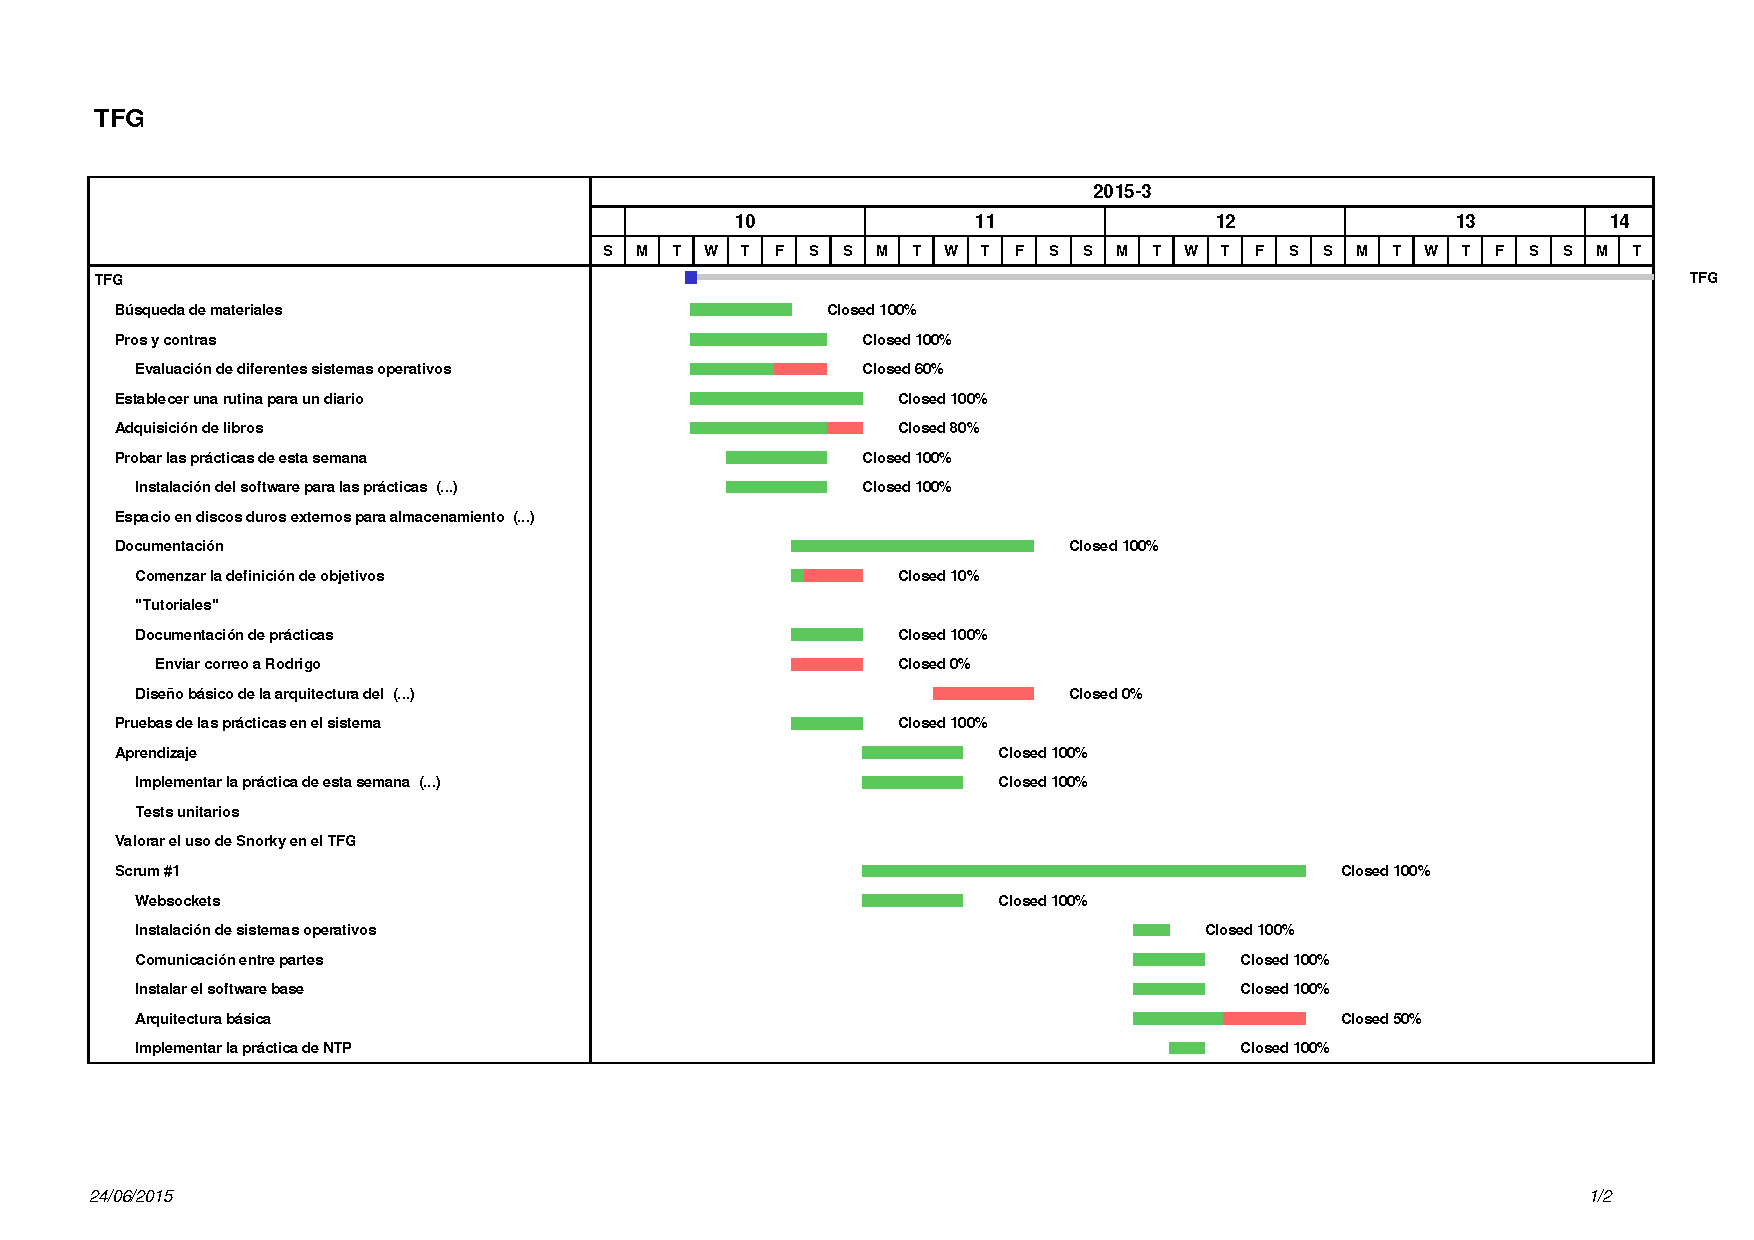
\includepdf[pages=1,pagecommand={},offset=-2.5cm -3cm]{Chapters/Chapter3/Figures/tfg-gantt-mar.pdf}
% \caption{Actividad realizada en el mes de marzo}
% \end{figure}
% \includepdf[pages=2,pagecommand={},offset=-2.5cm -3cm]{Chapters/Chapter3/Figures/tfg-gantt-mar.pdf}
% 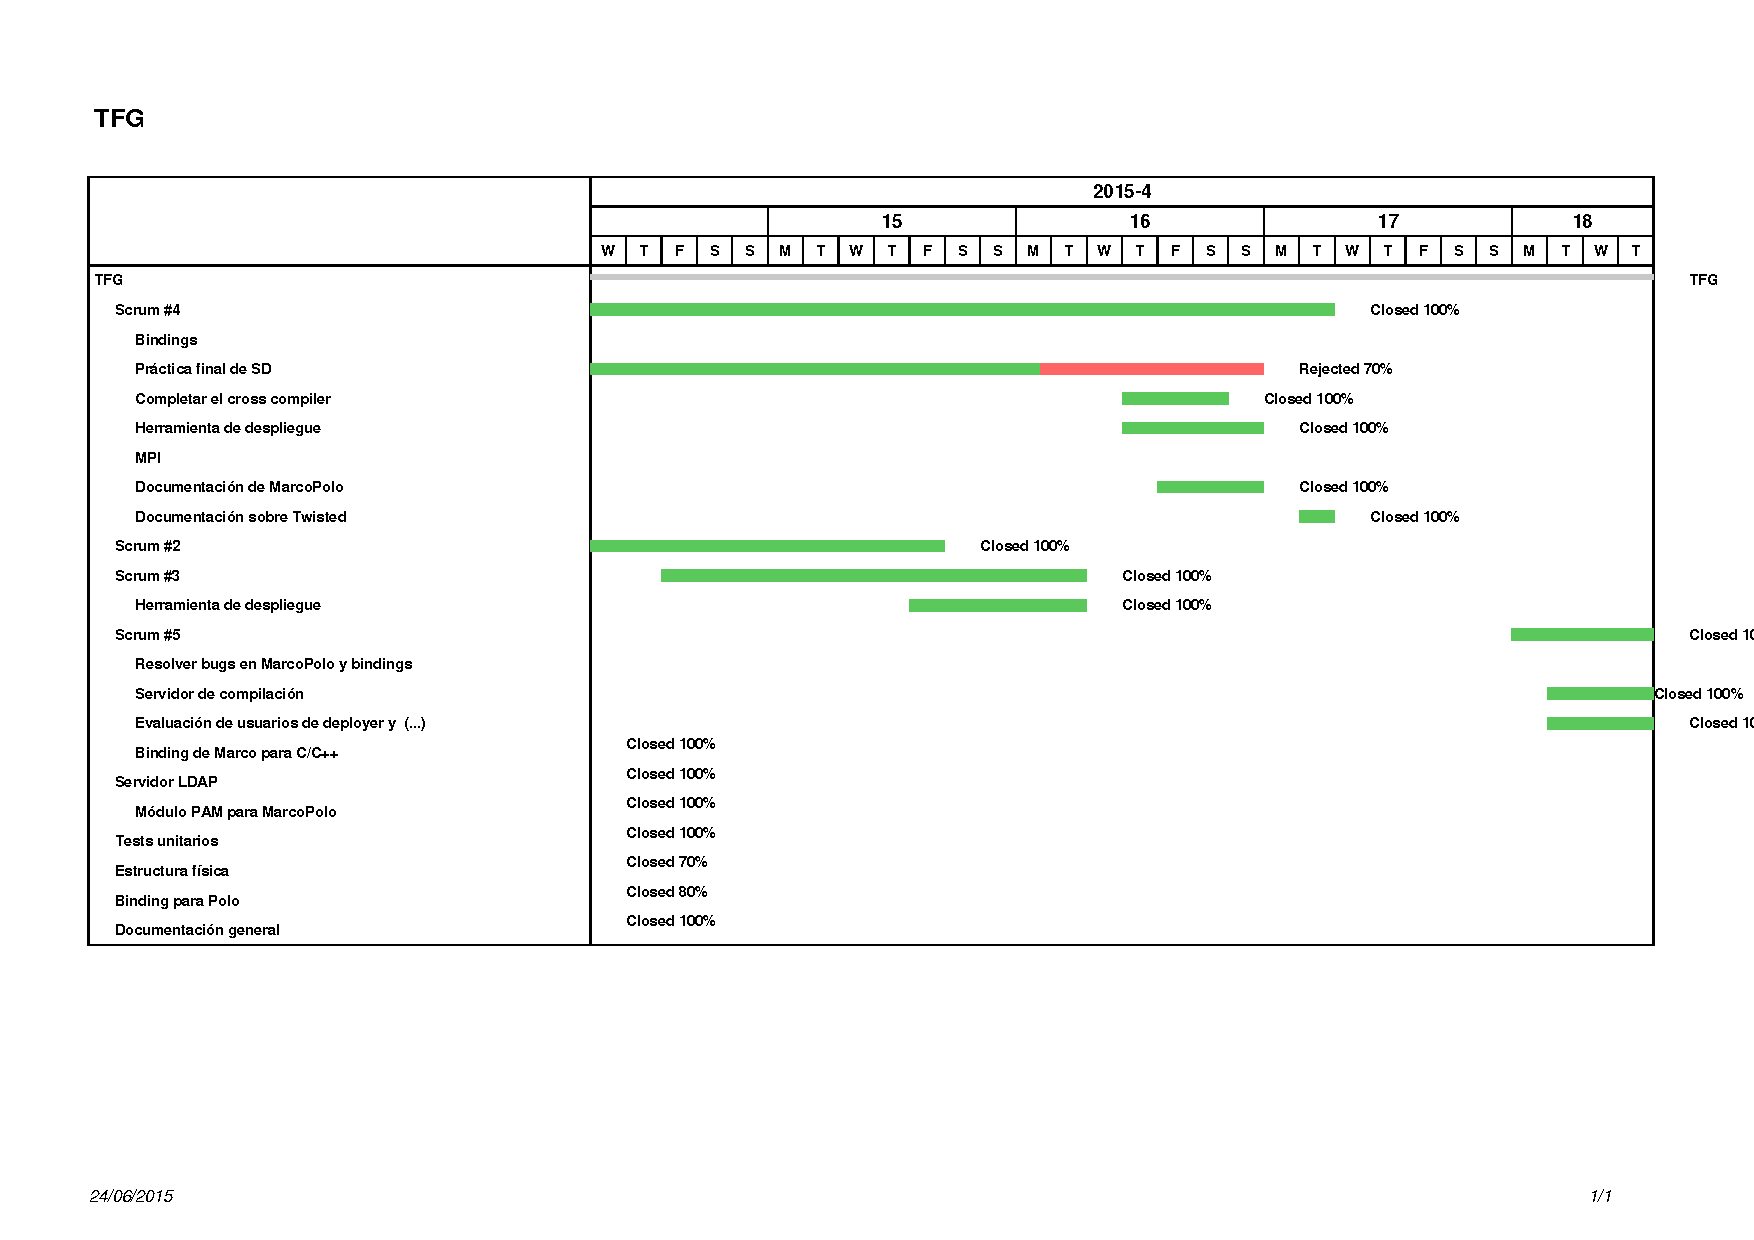
\includepdf[pages=1,pagecommand={},offset=-2.5cm -3cm]{Chapters/Chapter3/Figures/tfg-gantt-apr.pdf}
% 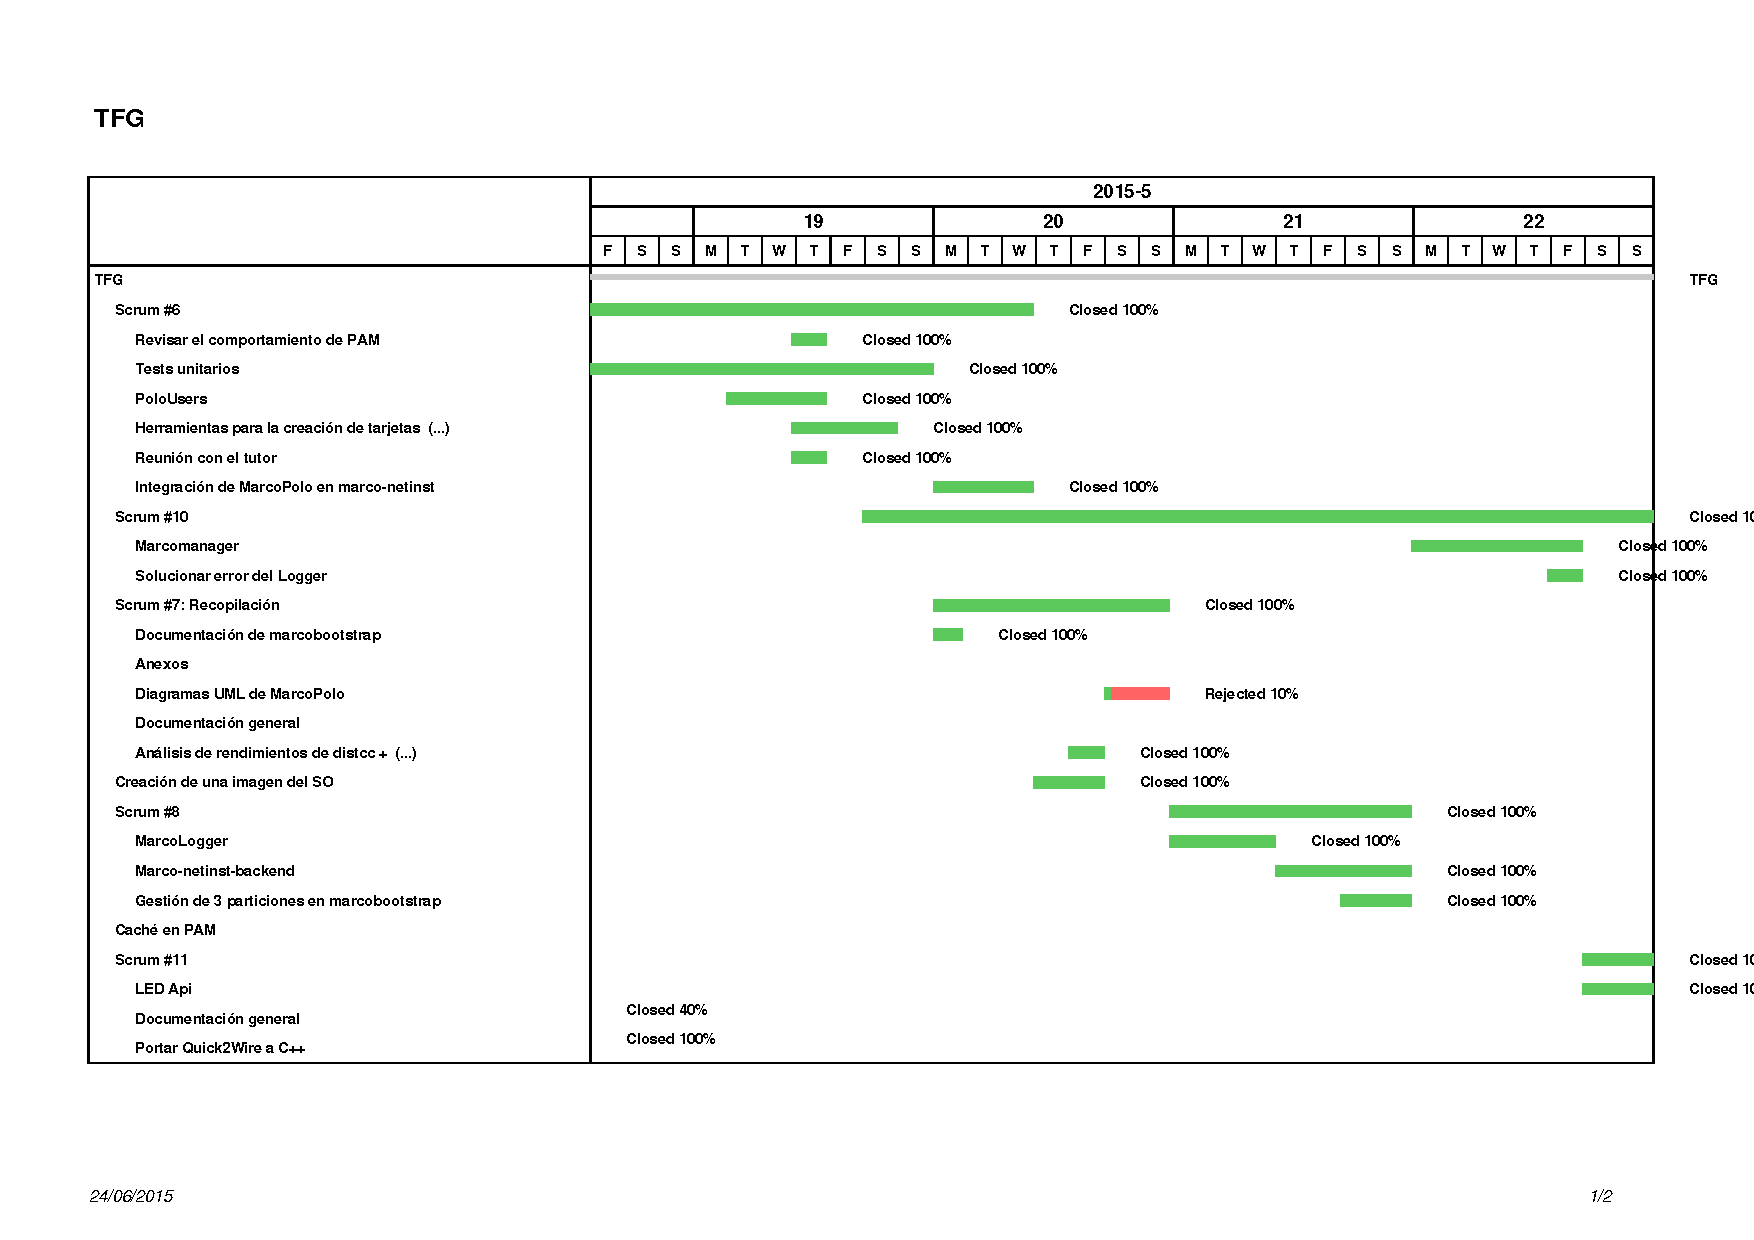
\includepdf[pages=1,pagecommand={},offset=-2.5cm -3cm]{Chapters/Chapter3/Figures/tfg-gantt-may.pdf}
% \includepdf[pages=2,pagecommand={},offset=-2.5cm -3cm]{Chapters/Chapter3/Figures/tfg-gantt-may.pdf}
% 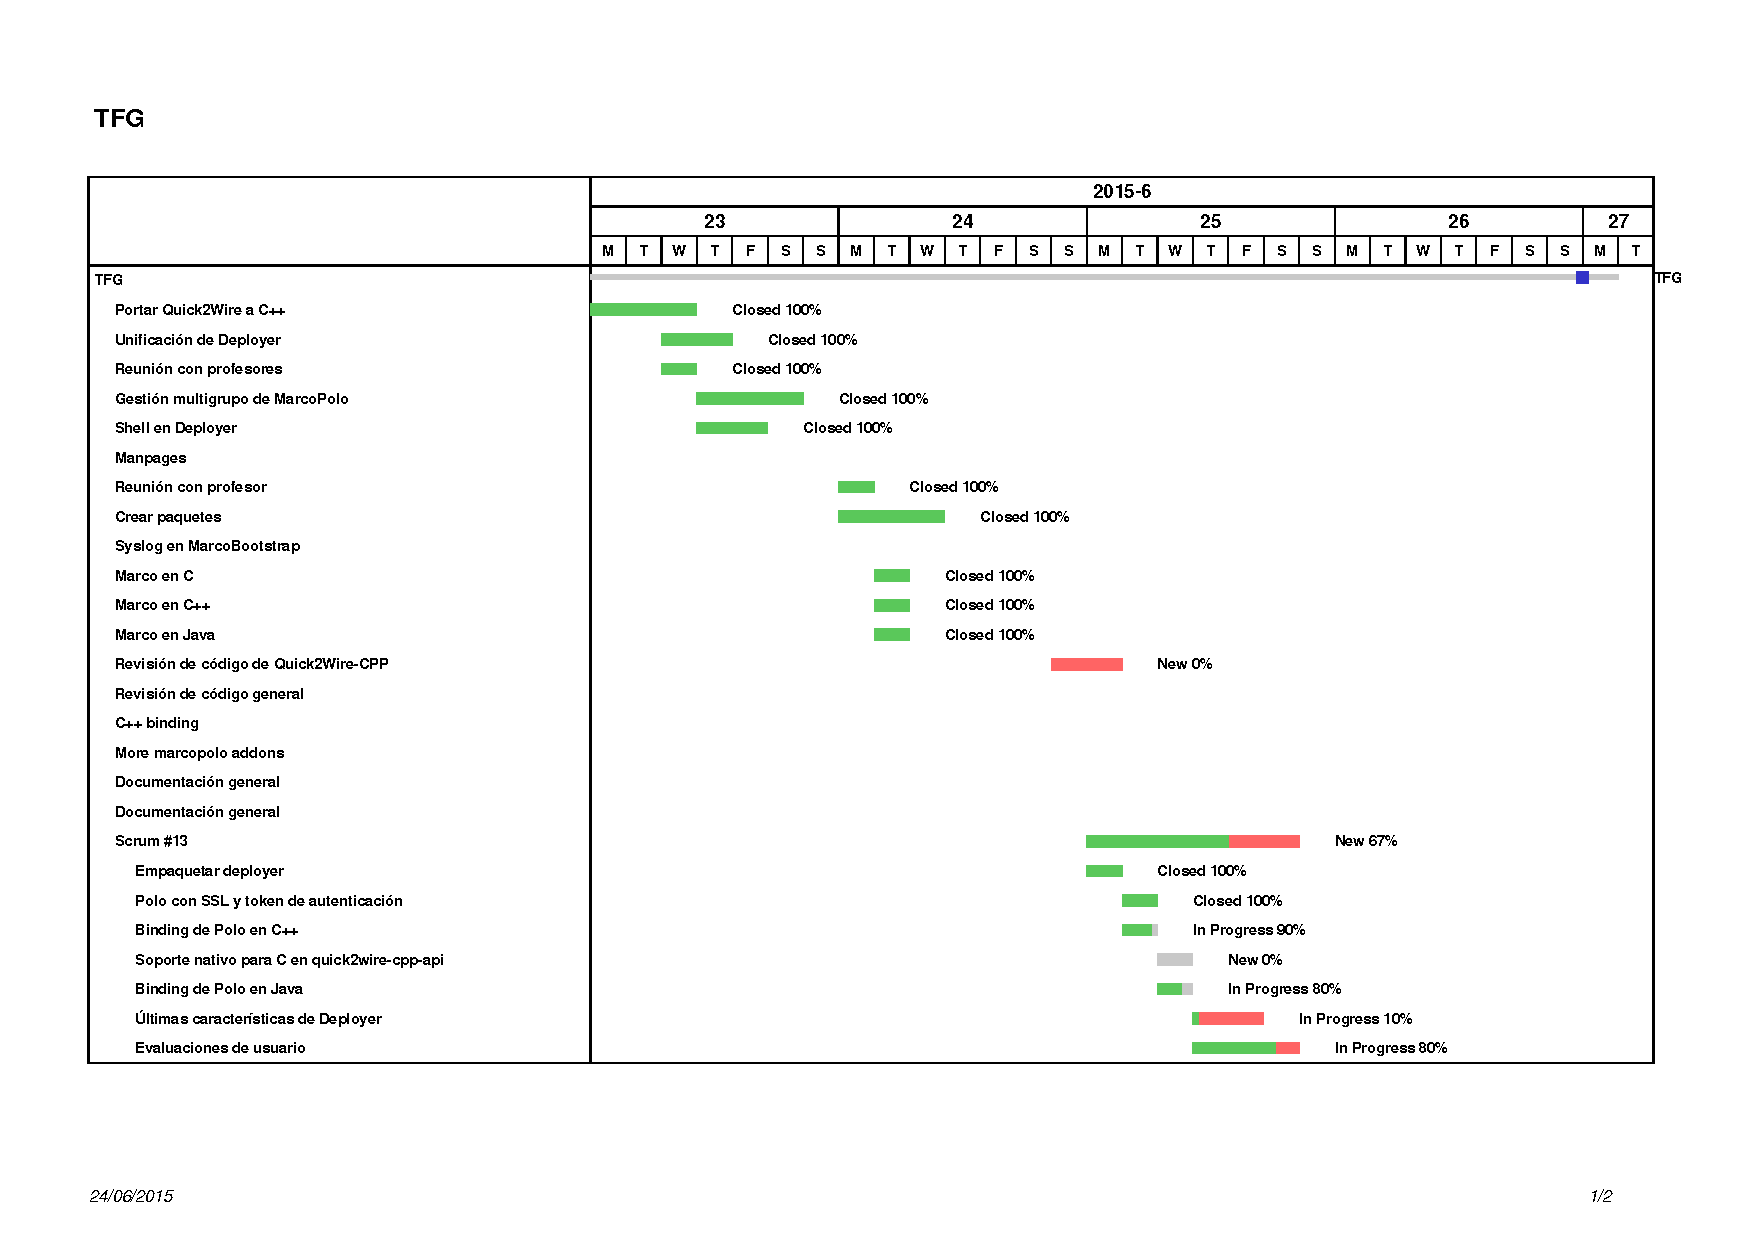
\includepdf[pages=1,pagecommand={},offset=-2.5cm -3cm]{Chapters/Chapter3/Figures/tfg-gantt-jun.pdf}
% \includepdf[pages=2,pagecommand={},offset=-2.5cm -3cm]{Chapters/Chapter3/Figures/tfg-gantt-jun.pdf}
% %\includepdf[pages=2,pagecommand={},offset=-2.5cm -3cm]{Chapters/Chapter3/Figures/tfg-gantt-apr.pdf}

\begin{figure}[H]
\centering
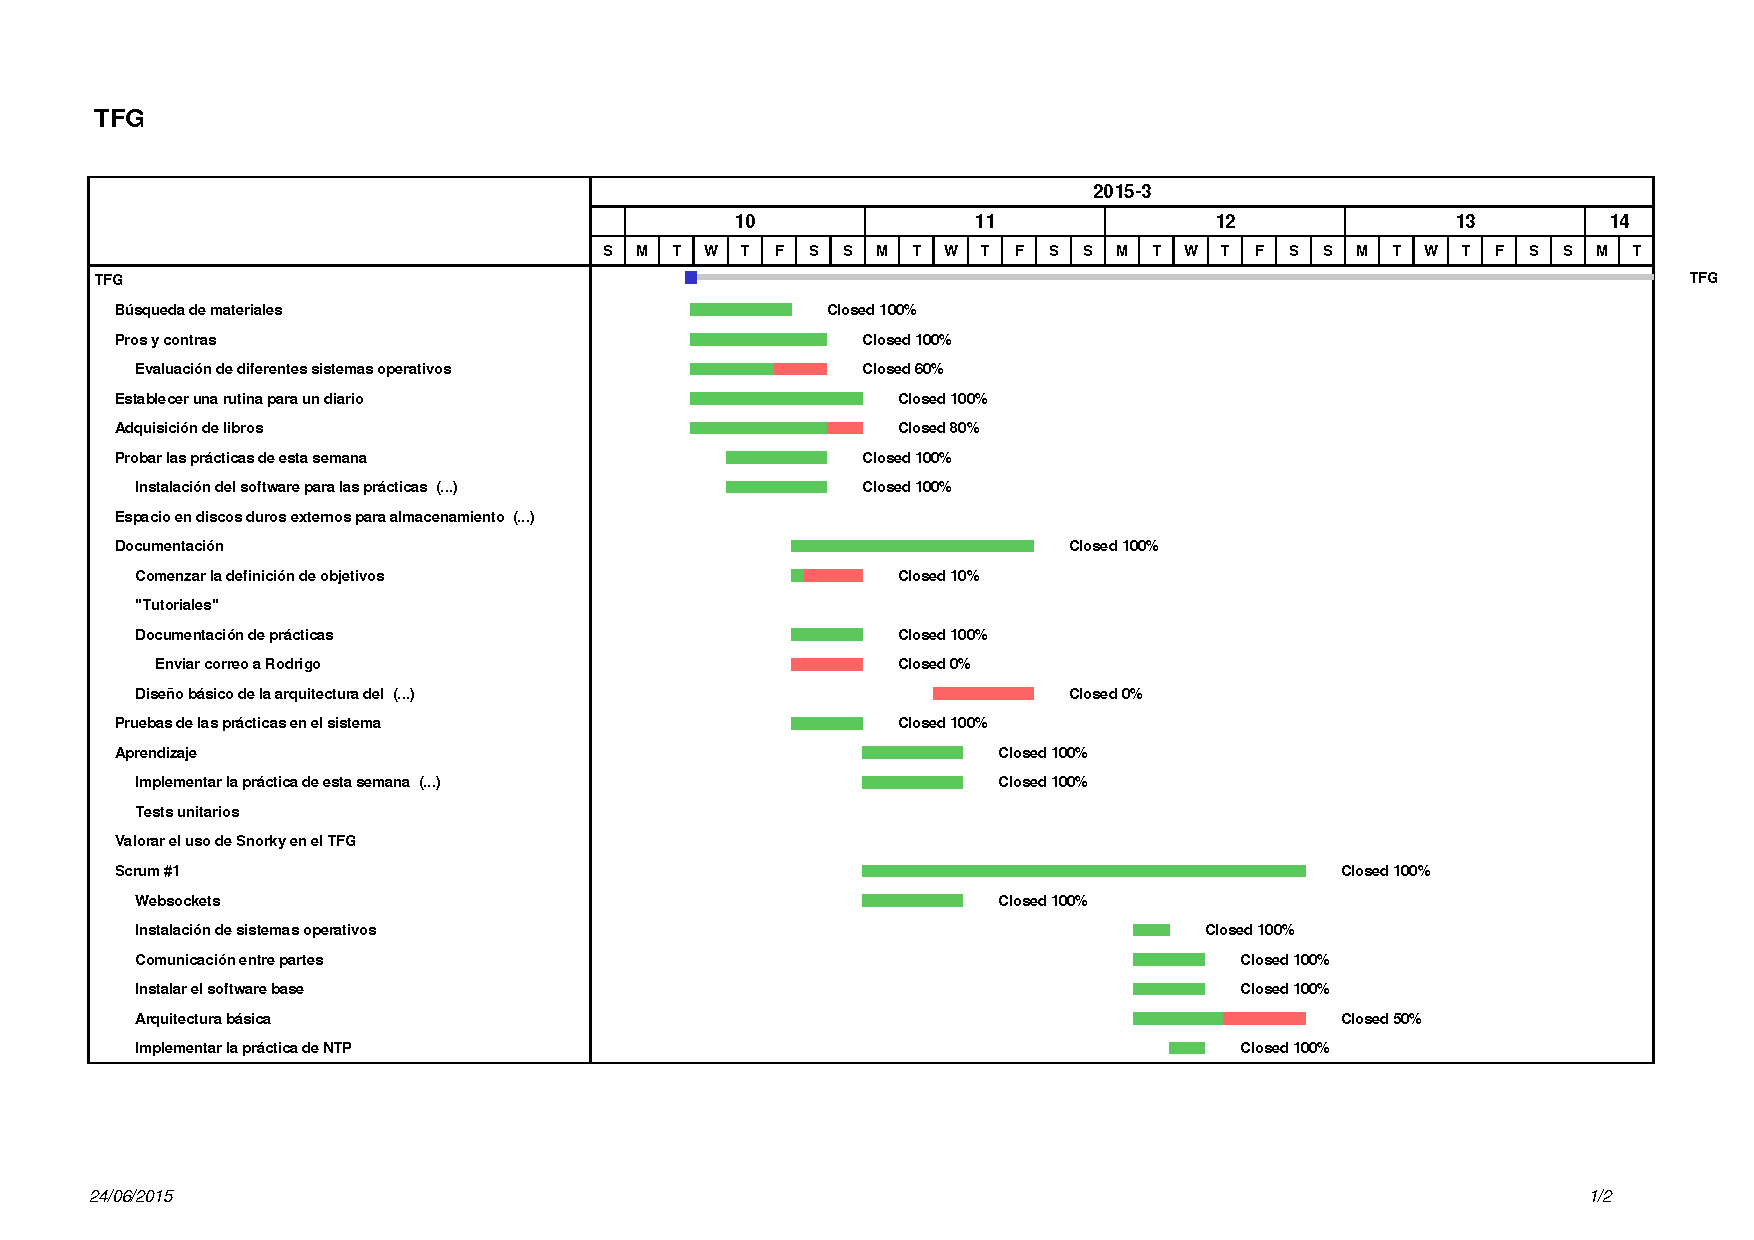
\includegraphics[width=0.7\textwidth]{Chapters/Chapter3/Figures/tfg-gantt-mar}
\end{figure}

\begin{figure}[H]
\centering
\includegraphics[width=0.7\textwidth]{Chapters/Chapter3/Figures/tfg-gantt-apr}
\end{figure}
\begin{figure}[H]
\centering
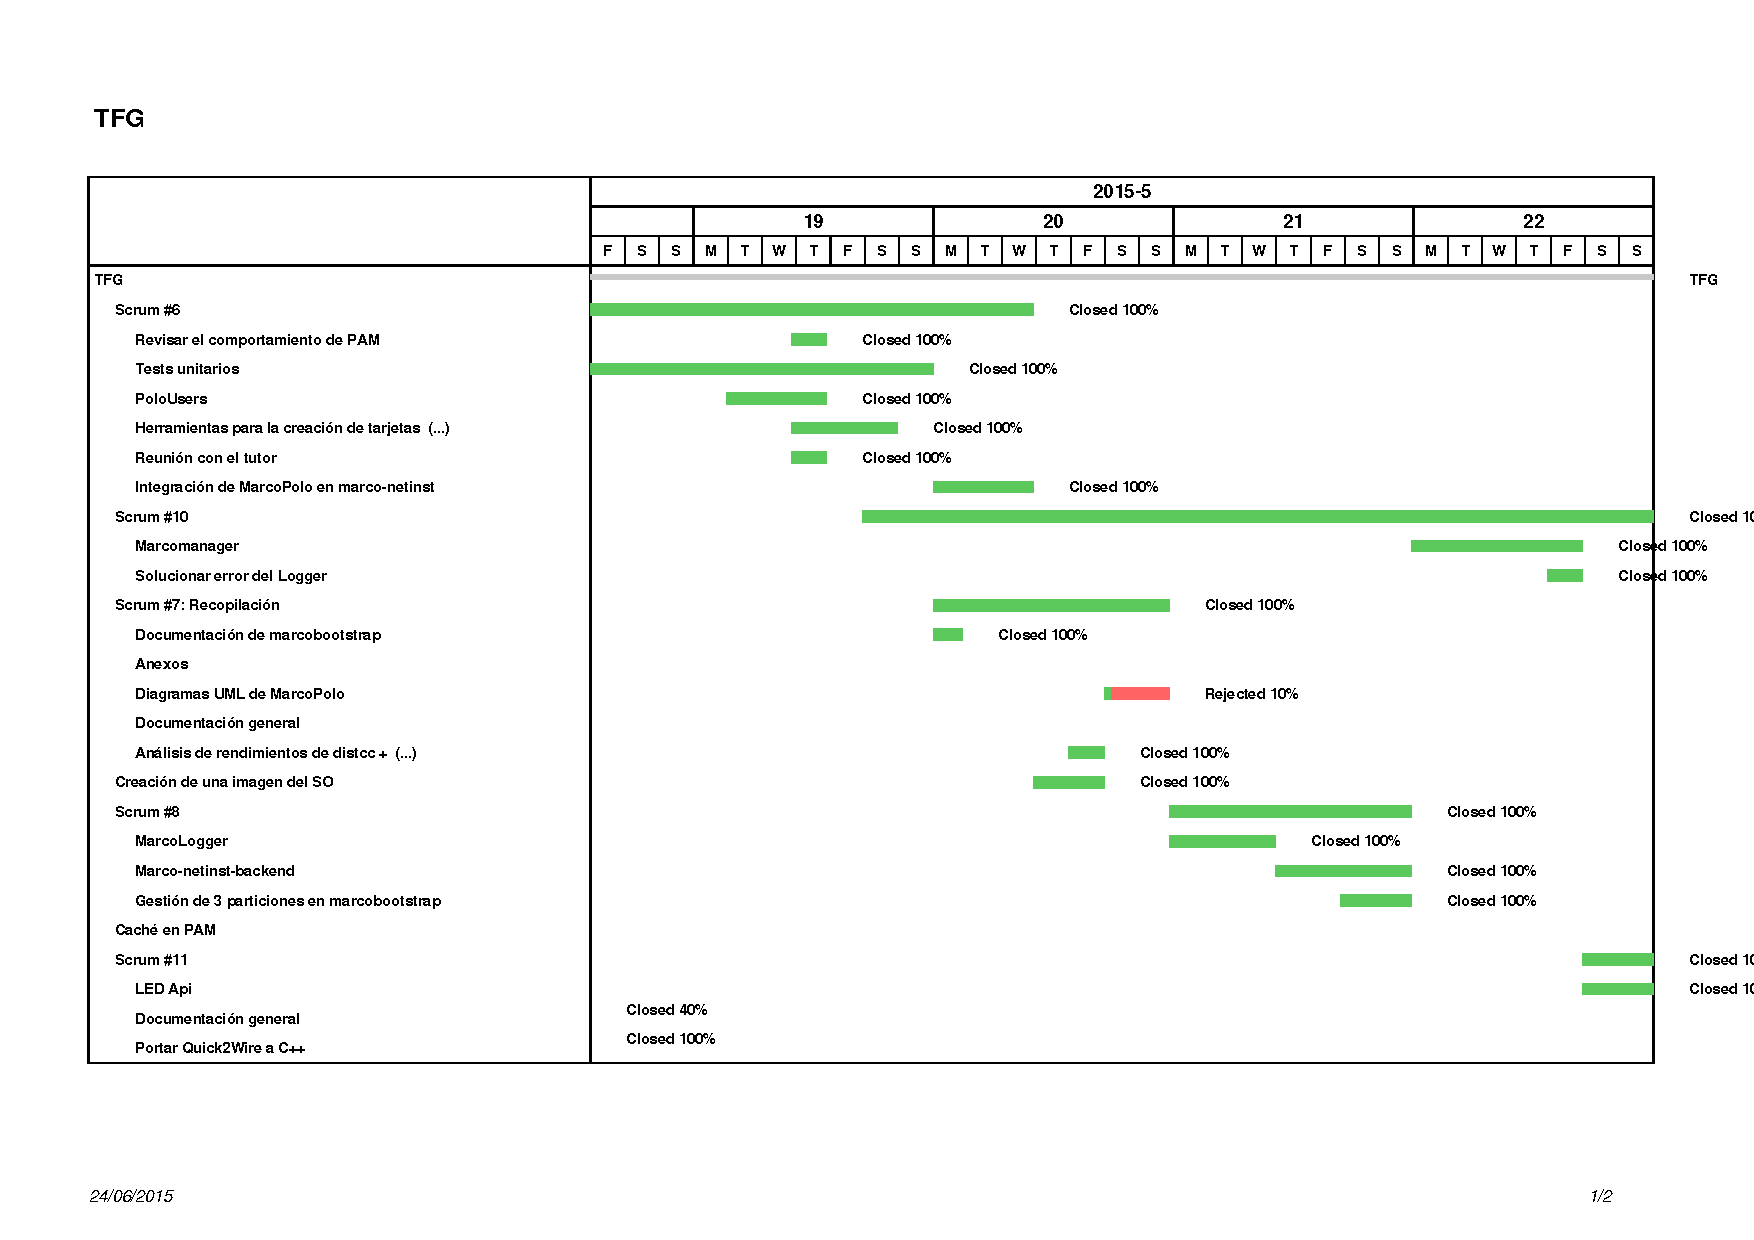
\includegraphics[width=0.7\textwidth]{Chapters/Chapter3/Figures/tfg-gantt-may}
\end{figure}
\begin{figure}[H]
\centering
\includegraphics[width=0.7\textwidth]{Chapters/Chapter3/Figures/tfg-gantt-jun}
\end{figure}

\chapter{Análisis y diseño}
\lhead{Análisis y diseño}
\label{chapter:analisis}

\section{Análisis}
\begin{cabstract}
En el que se describen los diferentes aspectos de la fase de análisis del sistema desde una perspectiva holística.
\end{cabstract}

Recoger todos los aspectos de análisis de un sistema como el creado en un único capítulo es contraproducente para la adecuada comprensión de los diferentes procesos llevados a cabo. Es por ello que en el presente capítulo se detallarán los diferentes aspectos de análisis llevados a cabo para el sistema como unidad, que ayudarán a la identificación de las necesidades a satisfacer por el mismo. Dichos aspectos serán de utilidad durante el desarrollo de las restantes etapas de análisis centradas en cada uno de los diferentes componentes del sistema.

\subsection{Identificación de componentes}

Todo sistema se compone del conjunto de integrantes y las relaciones que estos mantienen entre ellos mismos y su entorno, con una serie de objetivos a cumplir a través de dichas interacciones. El límite entre el sistema y su entorno es de necesario estudio para comprender los diferentes procesos de  entrada y salida que se desarrollan.

\subsubsection{Componentes principales} 

Los componente principales del sistema son los nodos Raspberry Pi, que serán los encargados de la ejecución de las diferentes tareas solicitadas por los usuarios del sistema.

\subsubsection{Componentes secundarios}

En una primera instancia del proceso de análisis no se detalla ningún tipo de nodo secundario, delegando en los componentes principales del sistema todas las tareas a llevar a cabo.

Sin embargo, en las diferentes etapas de desarrollo se plantea el uso de varios componentes secundarios para la gestión de una serie de tareas cuya ejecución en el conjunto de componentes principales es dificultosa, o su delegación beneficia al conjunto de nodos principales. En cualquier caso, dichas tareas pueden ser asignadas a los componentes principales en cualquier momento (ver \ref{chapter:serviciosauxiliares}).

\begin{figure}[H]
  \centering
  \includegraphics[width=0.8\textwidth]{Chapter4/Figures/Análisis-Componentes}
  \caption[Análisis de componentes]{Análisis de componentes del sistema}
  \label{analisis:componentes}
\end{figure}

\subsubsection{Interconexión}

Se plantea el uso de cableado físico Ethernet para la comunicación entre los diferentes nodos. Este tipo de conexión es soportada por todos los componentes anteriormente mencionados, y se cuenta con dicho cableado en la infraestructura del centro (ver \ref{dominioproblema:infraestructura}).

\subsection{Información gestionada por el sistema}

Se plantea un conjunto de requisitos de información gestionados por el sistema pequeño, sin embargo de alta sensibilidad, que el siguiente conjunto de datos.

\subsubsection{Credenciales de usuario}

Claves de acceso al sistema. Generalmente estas se componen de un par usuario-contraseña. Sin embargo, también se contemplan sistemas alternativos, como la autenticación de en clave pública. La manipulación de la identidad del usuario también es un aspecto clave del sistema.

\subsubsection{Archivos personales}

Junto a las claves de usuario es necesario gestionar los diferentes ficheros de trabajo que los usuarios manipulen y almacenen en el sistema. Esto implica proporcionar los diferentes mecanismos de acceso a dichos datos y un mecanismo de privilegios (lectura, escritura, ejecución) para impedir la manipulación de forma no deseada de los mismos.

\subsubsection{Ficheros de configuración e información del sistema}

Diversos componentes del sistema utilizan mecanismos de cifrado cuyas claves no deben ser conocidas por ninguna entidad mas que el administrador del sistema. Los ficheros de configuración del sistema y de las diversas aplicaciones a construir no deben ser modificables por usuarios no autorizados, pues definen aspectos del comportamiento del sistema que pueden comprometer la integridad del mismo si son modificados con fines perniciosos.

\subsubsection{Registros}

Diversos registros del comportamiento del sistema y de las operaciones realizadas en el mismo serán almacenados en el sistema para su posterior análisis. Dichos ficheros pueden incluir información sensible, como datos de usuarios, por lo que el acceso a los mismos deberá estar restringido.

\subsubsection{Información de estado}

Si bien la mayor parte de la información se describe en ficheros de carácter permanente, una parte de la información de importancia en el sistema es generada y gestionada por las propias aplicaciones sin almacenar la misma en ningún tipo de soporte permanente. La volatilidad de la información hace que la versatilidad de la misma sea mayor, sin embargo, será necesario contar con una serie de mecanismos que preserven la información frente a circunstancias como recargas de información, reinicios. La manipulación de este tipo de información (actualizaciones, consulta, modificación) presenta una serie de aspectos diferentes a los propios de las estructuras de datos tradicionales.

\subsubsection{Equipo de soporte}

Como equipos de soporte se plantea el uso del almacenamiento presente en los nodos principales, utilizando, en caso de que sea conveniente, algún nodo secundario como almacén de información.

\section{Identificación de transacciones}

Se plantea el siguiente flujo de transacciones por unidad de tiempo, basado en las estadísticas del sistema (ver \ref{dominio:estadisticast}). La frecuencia de estas operaciones se debe determinar en fases posteriores según estos datos.

\begin{itemize}
\item Operaciones de usuario
\subitem Autenticación contra el sistema.
\subitem Proceso de ficheros.
\subitem Generación de trabajos a realizar por el sistema.
\subitem Realización de pruebas de algoritmos y despliegues.
\item Operaciones de administración.
\subitem Actualizaciones del sistema.
\subitem Operaciones rutinarias de mantenimiento.
\subitem Acceso y análisis de registros.
\end{itemize}

\subsection{Evolución del sistema}

En caso de proporcionar una solución exitosa para el conjunto de problemas a resolver por el sistema, es esperable un incremento en el número de componentes principales con el fin de aumentar su capacidad de cómputo. Por ello, la escalabilidad del sistema debe ser uno de los requisitos fundamentales del mismo.

\subsection{Adquisición del sistema}

Los aspectos de la adquisición de los diferentes componentes se definen en \ref{adquisicion}

\subsection{Identificación de usuarios}

Los siguientes usuarios harán uso del sistema de forma directa o indirecta:

\subsubsection{Desarrolladores}

Son aquellos individuos que utilizan el sistema como herramienta de creación y prueba de aplicaciones distribuidas.

\subsubsection{Estudiantes}

Utilizan la plataforma como herramienta para la elaboración de trabajos académicos relacionados con el área de conocimiento de la computación distribuida y como mecanismo para facilitar el estudio de dicha rama.

\subsubsection{Profesorado}

Docentes de las áreas anteriormente mencionadas, que utilizarán el sistema para planificar diferentes ejercicios didácticos a resolver por los alumnos.

\subsubsection{Administradores}

Realizan tareas de mantenimiento en el sistema.

\vspace{1.5cm}

En los diferentes documentos de análisis adjuntos se detalla la interacción de cada entidad con cada uno de los componentes del sistema de forma más detallada, sirviendo esta enumeración como vista global de los diferentes agentes.

\section{Diseño}

%\section{Portada}
%\section{Lista de cambios}
%\section{Tabla de contenidos}
%\section{Lista de figuras}
%\section{Lista de tablas}
\subsection{Introducción}
\subsection{Ámbito del software}
\subsection{Diseño de datos}
\subsection{Diseño arquitectónico}
\subsection{Diseño de la interfaz}
\subsection{Diseño procedimental}
\subsection{Referencia cruzada a los requisitos}
\subsection{Pruebas}
\subsection{Entorno tecnológico del sistema}
\subsection{Plan de desarrollo e implementación}
%\section{Glosario}
%\section{Apéndices}


\subsection{Adquisición del sistema}

Antes de realizar cualquier operación de adquisición de componentes es necesario analizar diferentes factores, como las diferentes alternativas viables o soluciones de coste menor o incluso nulo.

En el caso del presente proyecto, la adquisición de una serie de componentes no es opcional, debido a que no se cuenta con ellos previamente. Tras plantear diferentes opciones sin coste, se decide adquirir los siguientes componentes:

\begin{itemize}
  \item Nodos \textbf{Raspberry Pi}.
  \item Cables de alimentación.
  \item Tarjetas SD/micro-SD (soporte de almacenamiento de la Raspberry Pi).
  \item Elementos estructurales.
\end{itemize}

En la fase inicial, se evalúa un gran número de opciones atendiendo a los siguientes criterios:

\begin{itemize}
  \item Prestaciones.
  \item Precio.
  \item Potencial tiempo de uso.
  \item Tiempo de entrega\footnote{Las restricciones de tiempo que el proyecto implica exigen tiempos que los materiales sean entregados en un periodo de tiempo corto}.
\end{itemize}

%TODO
\citationneeded[TODO]
El proceso de compra de los diferentes componentes necesarios para el sistema se ha realizado de forma incremental, comenzando por una compra de tamaño significativo que incluye los diferentes componentes del sistema y posteriormente adquiriendo los componentes supletorios necesarios.

Esta estrategia ha permitido refinar las necesidades inicialmente planteadas, lo cual ha reducido significativamente el coste, al poder evaluar alternativas de igual efectividad y menor coste o incluso buscar mecanismos para reutilizar componentes con los que ya se contaba.

\begin{landscape}
\begin{table}
\begin{tabular}{|l|r|l|l|p{4.5cm}|p{5cm}|}
\hline
Ítem&Unidades&Precio/ud.&Total&Notas&Referencia\\
\hline
Raspberry Pi B+&4&€25.84&€103.36&Disponible para entrega en 2 día(s) laborable(s).&http://es.rs-online.com/web/p/kits-de-desarrollo-de-procesador-y-microcontrolador/8111284/?origin=PSF\_431027|alt\\
\hline
Raspberry Pi Rev 2&4&€30.58&€122.32&Temporalmente fuera de stock. Disponible a partir del 20/04/2015, con entrega en 2 día(s) laborable(s).&http://es.rs-online.com/web/p/kits-de-desarrollo-de-procesador-y-microcontrolador/8326274/\\
\hline
Rasbperry Pi B&4&€26.05&€104.20&&es.rs-online.com/web/p/kits-de-desarrollo-de-procesador-y-microcontrolador/7568308/\\
\hline
\end{tabular}
\caption{Coste de cada uno de los diferentes modelos de placa Raspberry Pi}
\end{table}
\end{landscape}

\definecolor{LightCyan}{rgb}{0.88,1,1}
\begin{landscape}
\begin{table}
\begin{tabular}{|l|r|l|l|l|p{3.5cm}|p{4.5cm}|}
\hline
Tarjetas SD\footnote{Únicamente compatibles con el modelo B}&Unidades&Precio/ud.&Total&Clase\footnote{La clase de una tarjeta define su velocidad de lectura y escritura, siendo representada por un múltiplo de 2. Ver\href{https://www.sdcard.org/developers/overview/speed_class/}{https://www.sdcard.org/developers/overview/speed\_class/}}&Notas&Referencia\\
\hline
8GB SD Card, Raspberry Pi NOOBS 1.4&4&€10.23&€40.92&Desconocida&Temporalmente fuera de stock. Disponible a partir del 30/04/2015, con entrega en 2 día(s) laborable(s).&http://es.rs-online.com/web/p/tarjetas-sd/8492012/\\
\hline
SDHC Kingston 16 GB Clase 10&4&€23.44&€93.76&Clase 10&Disponible para entrega en 24 horas.&http://es.rs-online.com/web/p/tarjetas-sd/7595577/\\
\hline
4GB SDHC Class 4 Flash Card&4&€5.83&€23.32&Clase 4&&http://es.rs-online.com/web/p/tarjetas-sd/6957325/\\
\hline
8GB SD Card, Raspberry Pi NOOBS 1.4&4&€10.23&€40.92&Desconocida&Temporalmente fuera de stock. Disponible a partir del 30/04/2015, con entrega en 2 día(s) laborable(s).&http://es.rs-online.com/web/p/tarjetas-sd/8492012/\\
\hline
8 GB SDHC&4&€15.49&€61.96&Class 10&&http://es.rs-online.com/web/p/tarjetas-sd/7582574/\\
\hline
16GB SDHC&4&€15.54&€62.16&Class 4&&http://es.rs-online.com/web/p/tarjetas-sd/6957337/\\
\hline
SDHC Kingston 16 GB Clase 10&4&€23.44&€93.76&Clase 10&Disponible para entrega en 24 horas.&http://es.rs-online.com/web/p/tarjetas-sd/7595577/\\
\hline
4GB SDHC Class 4 Flash Card&4&€5.83&€23.32&Clase 4&&http://es.rs-online.com/web/p/tarjetas-sd/6957325/\\
\hline
\end{tabular}
\newline
\end{table}
\end{landscape}
\begin{landscape}
\begin{table}
\begin{tabular}{|l|r|l|l|l|p{3.5cm}|p{4.5cm}|}
\rowcolor{LightCyan}
16 GB Verbatim Clase 10&4&€14.01&€56.04&Clase 10&&http://es.rs-online.com/web/p/tarjetas-sd/7504795/\\
\hline
8GB Verbatim&4&€7.80&€31.20&Clase 4&&http://es.rs-online.com/web/p/tarjetas-sd/7504789/\\
\hline
8GB SD Card&4&€10.23&€40.92&¿?&&http://es.rs-online.com/web/p/tarjetas-sd/8384842/\\
\hline
8GB SDHC Class 4&4&€8.58&€34.32&Class 4&&http://es.rs-online.com/web/p/tarjetas-sd/6957331/\\
\hline
8GB Lexar MicroSD&4&€12.59&€50.36&Class 4&&http://es.rs-online.com/web/p/tarjetas-sd/6661689/\\
\hline
4 GB Verbatim&4&€5.16&€20.64&Class 4&&http://es.rs-online.com/web/p/tarjetas-sd/7504770/\\
\hline
4GB SDHC&4&€11.36&€45.44&Class 10&&http://es.rs-online.com/web/p/tarjetas-sd/7582571/\\
\hline
\rowcolor{LightCyan}
8GB Class 10 SD Card&4&€8.84&€35.36&Class 10&&http://es.rs-online.com/web/p/tarjetas-sd/8006700/\\
\hline
\end{tabular}
\caption{Precios de diferentes modelos de tarjeta SD}
\end{table}
\end{landscape}

\begin{landscape}
\begin{tabular}{|l|l|l|l|l|l|l|l|l|}
\hline
MicroSD\footnote{compatibles con modelos B+/Rev 2 y modelo B utilizando un adaptador}&&&&&&\\
\hline
4GB microSDHC Class 4 Flash Card&4&€5.92&€23.68&Clase 4&&http://es.rs-online.com/web/p/tarjetas-sd/6957321/\\
\hline
MicroSDHC Verbatim 8GB Clase 4&4&€7.29&€29.16&Class 4&&http://es.rs-online.com/web/p/tarjetas-sd/7504786/\\
\hline

8GB microSDHC Class 4 Flash Card&4&€7.45&€29.80&Class 4&&http://es.rs-online.com/web/p/tarjetas-sd/6957334/&&\\
\hline
4 GB Trascend Micro SDHC&4&€6.52&€26.08&Clase 4&&http://es.rs-online.com/web/p/tarjetas-sd/7582593/&&\\
\hline
4GB MiniSD Lexar Media Card&4&€7.62&€30.48&Clase 2&&http://es.rs-online.com/web/p/tarjetas-sd/0540804/&&\\
\hline
4GB Verbatim MicroSDHC Clase 4&4&€6.71&€26.84&Class 4&&http://es.rs-online.com/web/p/tarjetas-sd/7504782/&&\\
\hline
\rowcolor{LightCyan}
Kingston 4 GB Clase 10&4&€8.54&€34.16&Class 10&&http://es.rs-online.com/web/p/tarjetas-sd/7595574/&&\\
\hline
\rowcolor{LightCyan}
Kingston 8GB Clase 10&4&€15.21&€60.84&Class 10&&http://es.rs-online.com/web/p/tarjetas-sd/7595583/&&\\
\hline
4GB Micro SDHC Trascend&4&€9.08&€36.32&Class 10&&http://es.rs-online.com/web/p/tarjetas-sd/7582603/&&\\
\hline
Cableado Ethernet&&&&&&&&\\
\hline
Latiguillos 1m&4&€1.38&€5.52&&&http://es.rs-online.com/web/p/latiguillos-cat6/0411227/&&\\
\hline
&&&&&&&&\\
\hline
Fuente de alimentación&&&&&&&&\\
\hline
\end{tabular}
\end{landscape}
\begin{landscape}
\begin{tabular}{|l|l|l|l|l|l|l|l|l|}
Totales&&&&&&&&\\
\hline
Raspberry Pi B, Tarjeta SD, Ethernet&€145.08&&&&&&&\\
\hline
Raspberry Pi B+, Tarjetas MicroSD, Ethernet&€169.72&&&&&&&\\
\hline
Raspberry Pi Rev 2, Tarjetas MicroSD, Ethernet&€188.68&&&&&&&\\
\hline
&&&&&&&&\\
\hline
&&&&&&&&\\
\hline
&&&&&&&&\\
\hline
Notas&&&&&&&&\\
\hline
Tarjetas SD:&&&&&&&&\\
\hline
\end{tabular}
\end{landscape}
%TODO SD/SDHC/SDXC: Las tarjetas HC (High capacity) garantizan una velocidad mínima de funcionamiento, indicado en la Clase de la tarjeta o en múltiplos de 150 kB/s&&&&&&&&\\
% \hline
% &&&&&&&&\\
% \hline
% Velocidad de transferencia según cada clase:&&&&&&&&\\
% \hline
% 2: 2MB/s&&&&&&&&\\
% \hline
% 4: 4MB/s&&&&&&&&\\
% \hline
% 6: 6MB/s&&&&&&&&\\
% \hline
% 10:10MB/s&&&&&&&&\\
% \hline
% \end{tabular}
% \end{landscape}

%\begin{landscape}
\begin{table}[H]
\begin{tabular}{|p{2.5cm}|p{2cm}|p{2cm}|p{2.5cm}|p{2.5cm}|p{2.5cm}|}
\hline
\textbf{Nombre} & \textbf{Unidades} & \textbf{Proveedor} & \textbf{Tiempo de entrega} & \textbf{Coste por unidad (€)} & \textbf{Total}\\ \hline
Raspberry Pi & 4 & Farnell & Una semana & 31.15 & suma\\ \hline

Separador de latón de 18 mm en pack de 25 & Comprobar & Comprobar & Comprobar & Comprobar & Comprobar\\ \hline
Cables USB & Comprobar & Comprobar & Comprobar & Comprobar & Comprobar\\ \hline
Tarjeta de memoria & 4 & Comprobar & Comprobar & Comprobar & Comprobar\\ \hline


\end{tabular}
\caption[Evaluación de precios de las diferentes alternativas para el proyecto]{Evaluación de precios de las diferentes alternativas para el proyecto}
%TODO:Todos los precios están basados en el coste unitario sin descuento por volumen y con IVA incluido reflejado en la web http://es.rs-online.com/web/&En verde la mejor opción de cada categoría&&&&&Referencia&&\\
\end{table}
%\end{landscape}


%TODO: IS 1 T2 pg 37
El coste total del proyecto no es elevado, por lo que no se solicitarán más presupuestos ni proveedores de los aquí listados. % Dominio del problema

\lhead{Arquitectura física}
\chapter{Arquitectura física} % Aspectos relevantes del desarrollo

\chapter{Conclusiones y líneas de trabajo futuro}
\lhead{\emph{Conclusiones y líneas de trabajo futuro}}

\begin{cabstract}

En el que se realiza un análisis retrospectivo de todas las etapas del Trabajo de Fin de Grado valorando los diferentes aspectos de las mismas y los resultados finales. Se incluyen además una serie de propuestas de trabajo futuro para el equipo de desarrollo o potenciales interesados y tareas ya planeadas que complementan el Trabajo.

\end{cabstract}

El trabajo descrito en los anteriores capítulos ha probado ser de gran utilidad como síntesis de los conocimientos a adquirir según se plantea en el currículo del Grado en Ingeniería Informática de la Universidad de Salamanca. Además, el sistema ha permitido desarrollar expandir los conocimientos adquiridos en las asignaturas Sistemas Distribuidos, Redes de Computadores, Administración de Sistemas, Interacción Persona-Ordenador, Interfaces Gráficas de Usuario y Gestión de Proyectos.

Como proyecto, la gestión del mismo ha permitido realizar una aproximación más cercana a un proyecto ``real'' que cualquier otro trabajo del plan de estudios, aprendiendo a lidiar con una incertidumbre muy alta y compaginando etapas de aprendizaje con etapas de desarrollo. El modelo de desarrollo utilizado, una metodología ágil basada prototipos, ha probado ser una vía efectiva para las demandas y restricciones del proyecto.

Los resultados finales del sistema prueban que el desarrollo de sistemas distribuidos en hardware de bajo coste es factible e incluso ventajoso para diferentes propósitos. La relación rendimiento/coste es muy alta y sus características (como el puerto GPIO, o la pequeña demanda de espacio físico) pueden ser aprovechadas en un contexto didáctico, aportando nuevas herramientas que facilitarán la etapa de aprendizaje a los estudiantes de las asignaturas.

Sin embargo, todas las herramientas creadas son independientes de la plataforma donde se ejecutan (excepto aquellas que dependan del \textit{hardware} presente en los nodos, como la biblioteca \textbf{quick2wire-cpp-api} o \textbf{marco-netinst}), por lo que su integración en cualquiera de los equipos de las aulas de informática de la organización no requiere adaptaciones al código fuente.

\section{Líneas de trabajo futuro}

Se plantean las siguientes líneas de trabajo futuro:

\begin{itemize}
	\item Instalar de forma definitiva (en lugar de las instalaciones de prueba realizadas) el sistema en la organización.
	\item Analizar los resultados de la integración del sistema y sus herramientas en las asignaturas planteadas durante el curso académico 2015-2016.
	\item Añadir a \textbf{MarcoPolo} la funcionalidad de publicación activa de servicios (anunciando en la red la adición de un nuevo servicio), en lugar de la publicación pasiva actual.
	\item Consolidar el protocolo \textbf{MarcoPolo} como herramienta de descubrimiento de servicios, portándolo a sistemas como impresoras en red, dispositivos multimedia\dots y facilitar su uso en redes inalámbricas.
\end{itemize}

\citationneeded[TODO] % Conclusiones y líneas de trabajo futuro

%% ----------------------------------------------------------------
% Now begin the Appendices, including them as separate files

\addtocontents{toc}{\vspace{2em}} % Add a gap in the Contents, for aesthetics

\appendix % Cue to tell LaTeX that the following 'chapters' are Appendices

\chapter{Lista de anexos}
\lhead{Lista de anexos}
\label{listaanexos}
En este apéndice se detalla la lista de todos los anexos que complementan el presente documento.
\begin{itemize}[noitemsep]
\item Configuración de un sistema de compilación multiplataforma con distcc y aplicación de este en un entorno distribuido.
\item Evaluación del rendimiento del sistema en un entorno real.
\item Estructura física.
\item Gestión del proyecto.
\item Informes de viabilidad de las prácticas de la asignatura Sistemas Distribuidos.
\item Evaluación del rendimiento del sistema en un entorno real.
\item Anexos técnicos, detallando en cada uno de ellos la especificación de los requisitos del \textit{software}, especificación del diseño, documentación técnica, manuales de usuario y cualquier otro aspecto de relevancia.

\subitem Documentación técnica de MarcoPolo.
\subitem Documentación técnica de Marcodeployer.
\subitem Documentación técnica de PoloUsers.
\subitem Documentación técnica de MarcoBootstrap.
\subitem Documentación técnica de MarcoManager.
\subitem Documentación técnica de quick2wire-cpp-api y el resto de herramientas relacionadas.

\item Evaluaciones de usuario.
\item Pruebas del sistema.
\end{itemize}	% Appendix Title

%\chapter{Listado de paquetes}
\lhead{Listado de paquetes}
\label{paquetes} % Appendix Title

%\chapter{Listado de contenidos del DVD}
\lhead{Listado de contenidos del DVD}
\label{contenidosdvd} % Appendix Title

\chapter{Listado de repositorios de código}
\lhead{Listado de repositorios de código}
\label{repositorios}

Lista de los diferentes repositorios de git donde se encuentra todo el código de los productos \textit{software} realizados.


\begin{itemize}[noitemsep]
\item \href{https://bitbucket.org/Alternhuman/marcopolo}{https://bitbucket.org/Alternhuman/marcopolo}
\item \href{https://bitbucket.org/Alternhuman/deployer}{https://bitbucket.org/Alternhuman/deployer}
\item \href{https://bitbucket.org/Alternhuman/crosstool-conffiles}{https://bitbucket.org/Alternhuman/crosstool-conffiles}
\item \href{https://bitbucket.org/Alternhuman/memoria-tfg}{https://bitbucket.org/Alternhuman/memoria-tfg}
\item \href{https://bitbucket.org/Alternhuman/marco-netinst}{https://bitbucket.org/Alternhuman/marco-netinst}
\item \href{https://bitbucket.org/Alternhuman/marcopolo-bindings-cpp}{https://bitbucket.org/Alternhuman/marcopolo-bindings-cpp}
\item \href{https://bitbucket.org/Alternhuman/marcopolo-shell}{https://bitbucket.org/Alternhuman/marcopolo-shell}
\item \href{https://bitbucket.org/Alternhuman/quick2wire-gpio-admin}{https://bitbucket.org/Alternhuman/quick2wire-gpio-admin}
\item \href{https://bitbucket.org/Alternhuman/mpi\_led}{https://bitbucket.org/Alternhuman/mpi\_led}
\item (\textit{Fork}) \href{https://bitbucket.org/Alternhuman/quick2wire-python-api}{https://bitbucket.org/Alternhuman/quick2wire-python-api}
\item \href{https://bitbucket.org/Alternhuman/quick2wire-cpp-api}{https://bitbucket.org/Alternhuman/quick2wire-cpp-api}
\item \href{https://bitbucket.org/Alternhuman/marcopolo-cluster-estructura}{https://bitbucket.org/Alternhuman/marcopolo-cluster-estructura}
\item \href{https://bitbucket.org/Alternhuman/marcomanager}{https://bitbucket.org/Alternhuman/marcomanager}
\item \href{https://bitbucket.org/Alternhuman/polousers}{https://bitbucket.org/Alternhuman/polousers}
\item \href{https://bitbucket.org/Alternhuman/marcopolo-doc}{https://bitbucket.org/Alternhuman/marcopolo-doc}
\item \href{https://bitbucket.org/Alternhuman/marcopolo-bindings-python}{https://bitbucket.org/Alternhuman/marcopolo-bindings-python}
\item \href{https://bitbucket.org/Alternhuman/marcopolo-bindings-java}{https://bitbucket.org/Alternhuman/marcopolo-bindings-java}
\item \href{https://bitbucket.org/Alternhuman/tfg-utils/src}{https://bitbucket.org/Alternhuman/tfg-utils/src}

\textbf{Paquetes descontinuados cuya funcionalidad se ha integrado en otro repositorio}
\item \href{https://bitbucket.org/Alternhuman/marco-bootstrap}{https://bitbucket.org/Alternhuman/marco-bootstrap}.
\item \href{https://bitbucket.org/Alternhuman/statusmonitor}{https://bitbucket.org/Alternhuman/statusmonitor}

\end{itemize}
\lhead{Listado de puertos utilizados}
\chapter{Listado de puertos utilizados}

\begin{table}[H]
\centering
\begin{tabular}{|p{1.5cm}|l|p{7.5cm}|p{2cm}|}\hline
\textbf{Puerto}&\textbf{Protocolo}&\textbf{Uso}&\textbf{Interfaz}\\
\hline
1337&UDP&Puerto del demonio \textbf{Marco}&127.0.1.1\\
\hline
1338&UDP&Puerto de la instancia de \textbf{Polo}&IP del grupo suscrito\\
\hline
1390&TCP (TLS/SSL)&Puerto del bindings de \textbf{Polo}&127.0.0.1\\
\hline
1342&TCP (HTTPS)&Puerto de \textbf{Deployer}&eth0\\
\hline
1442&TCP (HTTP)&Puerto no seguro de \textbf{Deployer}&eth0\\
\hline
1339&TCP (HTTPS)&Puerto de \textbf{Receiver}&eth0\\
\hline
1370&TCP (WSS)&Puerto para los WebSockets de \textbf{receiver}&eth0\\
\hline
1343&TCP (TLS/SSL)&Puerto de \textbf{polousers}&eth0\\
\hline
1345&TCP (HTTPS)&Puerto de ficheros de \textbf{Marcobootstrap-backend}&eth0\\
\hline
1346&TCP (HTTPS)&Puerto de la interfaz web de \textbf{Marcobootstrap-backend}&eth0\\
\hline
1446&TCP (HTTP)&Puerto de la interfaz web de \textbf{Marcobootstrap-backend}&eth0\\
\hline
1360&TCP (HTTPS)&Puerto de \textbf{Marcobootstrap-receiver}&eth0\\
\hline
8080&TCP (HTTP)&Puerto de servicios de \textbf{Tomcat}&eth0\\
\hline
8005&TCP (HTTP)&Puerto de apagado de \textbf{Tomcat}&lo\\
\hline
<uid> + 10000&TCP (HTTP)&Puerto de servicios de \textbf{Tomcat} para un usuario&eth0\\
\hline
<uid> + 20000&TCP (HTTP)&Puerto de apagado de \textbf{Tomcat} para un usuario&lo\\
\hline
\end{tabular}
\caption{Listado de puertos utilizados en el sistema}
\label{ports}
\end{table}
%\newglossaryentry{pi}
{
  name={\ensuremath{\pi}},
  description={ratio of circumference of circle to its
               diameter},
  sort=pi
}

\printglossaries

\addtocontents{toc}{\vspace{2em}}  % Add a gap in the Contents, for aesthetics
\backmatter
\nocite{Coulouris:2011:DSC:2029110}
\nocite{insideappletalk}
\nocite{2004:GPM:1121729}
%% ----------------------------------------------------------------
\label{Bibliography}
\lhead{\emph{Bibliography}}  % Change the left side page header to "Bibliography"
\bibliographystyle{ieeetr}  % Use the "unsrtnat" BibTeX style for formatting the Bibliography
\bibliography{Bibliography}  % The references (bibliography) information are stored in the file named "Bibliography.bib"
%There are \arabic{undefinedreferences} undefined references
\end{document}  % The End
%% ----------------------------------------------------------------